\documentclass[journal]{IEEEtran}
\usepackage{amsmath,amsthm,amssymb}
\usepackage{color}
\usepackage{graphicx}
\usepackage{cite}
\usepackage{subfigure}
\usepackage{array}
\usepackage{diagbox}
%\usepackage{flushend}
\usepackage[ruled,linesnumbered]{algorithm2e}
\usepackage{multirow}
\usepackage{mathrsfs}

\def\BibTeX{{\rm B\kern-.05em{\sc i\kern-.025em b}\kern-.08em
    T\kern-.1667em\lower.7ex\hbox{E}\kern-.125emX}}
\usepackage{balance}
\usepackage{float}
\usepackage{stfloats}


%\setlength\arraycolsep{0.8pt}
\newcommand{\PreserveBackslash}[1]{\let\temp=\\#1\let\\=\temp}
\newcommand{\tabincell}[2]{\begin{tabular}{@{}#1@{}}#2\end{tabular}}
\newcolumntype{C}[1]{>{\PreserveBackslash\centering}m{#1}}
\newcolumntype{R}[1]{>{\PreserveBackslash\raggedleft}m{#1}}
\newcolumntype{L}[1]{>{\PreserveBackslash\raggedright}m{#1}}


\begin{document}
\title{Learning-Based Collaborative Trajectory Planning Algorithm for Multi-UAV IoT Data Collection}
\author{
\thanks{
	This work was supported in part by the 
%\vspace{-3ex}
}}

\markboth{Accepted by IEEE Internet of Things Journal, Oct.~2023}%
{  }

\maketitle

\begin{abstract}
Unmanned aerial vehicle (UAV) data collection plays a pivotal role in enhancing the functionality and reliability of wireless sensor networks (WSNs) in environments lacking communication infrastructure, such as forests, oceans, disaster areas, etc. In these applications, the trajectory planning for UAVs is a key technique to improve the network performance. However, for multi-UAV-enabled data collection in complex and dynamic environment, the trajectory planning presents significant challenges in partial observability of environment, multi-objective optimization and UAV collaboration. In this work, a collaborative multi-agent deep recurrent Q-network (DRQN)-based trajectory planning algorithm is proposed. Each UAV interacts with adjacent UAVs for environmental information exchange. In the proposed algorithm, the neural network decomposition is employed to independently process the local and neighboring environmental observation data, enabling a collaborative policy. Then, the long-short term memory (LSTM) that is embedded within the policy achieves precise trajectory planning under partial knowledge of environment by aggregating historical environmental information. Moreover, a hierarchical reward function architecture which includes fairness-oriented data collection reward functions is appropriately designed and employed in policy training, ultimately deriving an optimal multi-UAV trajectory planning for data collection. Comparing with the benchmark algorithms, the proposed algorithm exhibits improvement on time cost while ensuring high reliability, and achieves efficient and stable UAV collaboration. 
\end{abstract}

\begin{IEEEkeywords}
Trajectory planning, Unmanned aerial vehicle (UAV), Collaboration, Deep reinforcement learning, Deep recurrent Q-network (DRQN)
\end{IEEEkeywords}


\section{Introduction} \label{introduction}

Unmanned aerial vehicles (UAVs) serve as powerful enablers within the Internet of Things (IoT). They can be equipped as aerial communication and computing platforms and provide data transmission \cite{Chu23,ZYin24} and mobile edge computing (MEC) for IoT end devices \cite{Pervez24,Savkin23}. With its high mobility, the UAV provides wireless communications that demonstrate superior resilience to geographical constraints compared to terrestrial communication infrastructure, particularly in complex topographies such as post-disaster areas and alpine regions. As an aerial communication platform, its air-to-ground communication link has a grater probability of line-of-sight (LoS) wireless channel which improves the communication efficiency of IoT networks and reduces energy consumption \cite{Xiao22}. 

Wireless sensor network (WSN) that composed of large amount of IoT sensors has valuable applications, such as forest fire monitoring, smart agriculture and weather detection \cite{YChen24}. However, reliable and efficient data collection form the IoT sensors constitutes a challenge in some application scenarios due to the lack of base stations. As shown in Fig. \ref{scene}, leveraging the advantages of UAV, UAV-enabled data collection is a solution with high efficiency, few terrain restriction and low energy consumption to WSN \cite{ZWei22}. 
\begin{figure}[htp]
	\centering
	%	\setlength{\abovecaptionskip}{-0.03cm}
	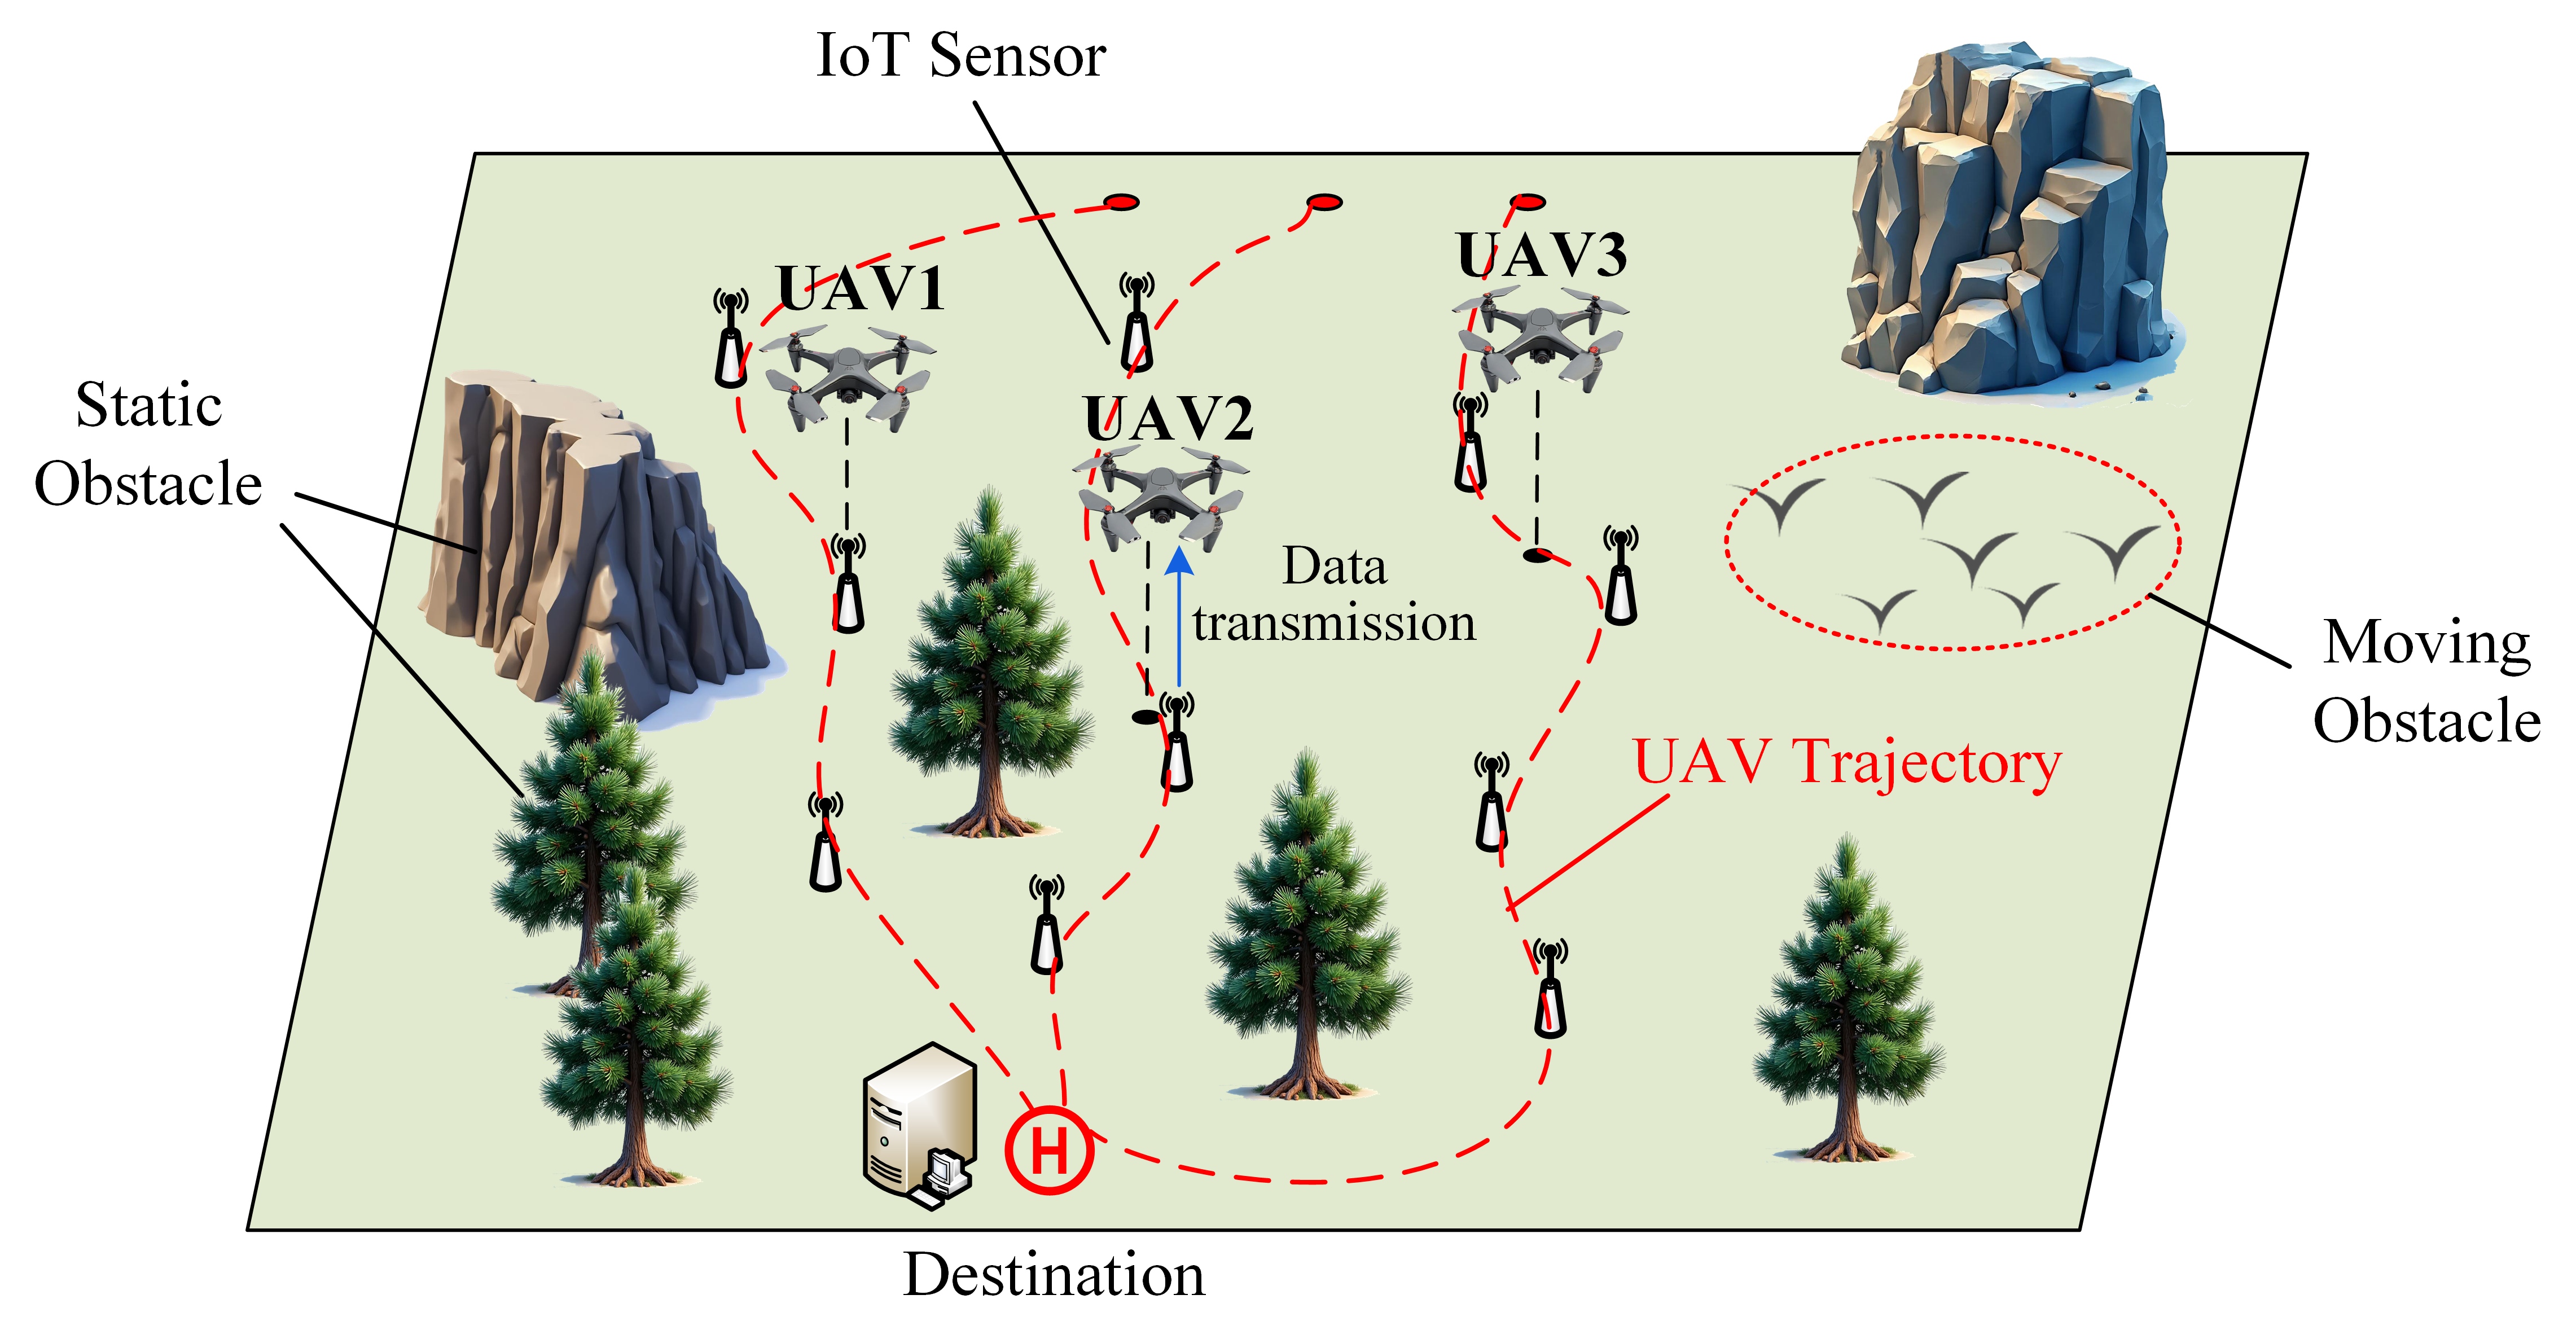
\includegraphics[width=0.48\textwidth]{fig/Sceme.png}
	\caption{The scenario of multi-UAV data collection for IoT sensor nodes in complex environment.\label{scene}}
\end{figure}

The trajectory of UAV in data collection is an issue that relates to the collection time and efficiency, age of information and energy consumption \cite{Cheng23}. Trajectory planning problem in UAV-assisted data collection can be regarded as the combination of navigation problem and collection scheduling problem. For collection scheduling problem, as an UAV need to serve several IoT nodes in most applications, an optimal collection sequence needs to be determined. Moreover, in multiple UAV-assisted data collection, the allocation of IoT nodes for each UAV has the effect on the efficiency of the whole system. For navigation problem, the UAV needs to be navigated to the position of IoT sensor nodes and the final landing position under the impact of obstacles in the environment. 
  %\textit{1)The collaboration of multiple UAVs}: As the collection task is jointly completed by multiple UAVs, the data collection workload of UAVs should be allocated evenly. With the certain amount of data needed to be collected, if any UAV has too much data to be collected, the data collection capability of other UAVs will be wasted. Moreover, as each UAV has the high mobility, the avoidance of collision with neighboring UAVs is one of the requirements in data collection task of multiple UAVs.
% 
%  \textit{2)Multiple optimization objects}: The data collection task contains multiple optimization objects, such as path length, data collection rate, energy consumption and collision rate. Multiple optimization objects are expected to be jointly optimized in some scenes. In multi-UAV task, the optimization points at the overall data collection performance of all the UAVs. 
%  
%  \textit{3)Partial observation of environment}: The UAV needs the information of environment to make its path decision. In the application with wide environment range or massive IoT nodes, as the UAV has the limited detection range of environment, the detection range of obstacles or IoT nodes is smaller than the environment space. The challenge for UAV is to find the overall optimal flying path within the limited sensing range of environment. 

%According to the above descriptions, developing a path planning algorithm for multiple UAV-assisted data collection that can overcome these challenges and realize the demanded optimization goals can improve the data collection efficiency and stability in large and complex environment. 

In recent years, various methods to solve trajectory planing problem for UAV-assisted data collection have been studied. For non-learning based methods, various articles modeled the problem as travelling salesperson problem (TSP). To realize data collection with optimization goals, the UAV trajectory is generated by deciding the visiting sequence of IoT node or a sequence of hovering collection positions \cite{Yan23,TWang22,YLi23,Shen22,MLi23,XHuang20}. The trajectory is generated by directly connecting the collection positions in sequence. Li et al. \cite{YLi23} developed algorithms for collection location planning in the consideration of different data collection modes. After UAV trajectory was decided, the altitude and velocity of UAV can be optimized to further reach the optimization goal \cite{JLi20}. If multiple UAVs had been deployed, the mission area dividing \cite{TWang22} and path segmentation \cite{XHuang20} was used for multiple UAV collaboration assignment. Wang et al. proposed a working area dividing method for multiple UAVs using K-mean algorithm. Although these methods can solve the path planing problem efficiently, they need comprehensive information of all the IoT nodes to compute the trajectory solution, which reduces the practicality of these methods in the environments that the location distribution of IoT nodes is unknown or dynamic, such as emergency search and rescue in disaster area. Then, these researches focused on single optimization objects. Few article studied multiple optimization objects simultaneously. Additionally, the collaboration assignment of UAVs is inflexible. If any one UAV malfunctioned, other normal UAVs cannot take over its collection work. Hence, these path algorithms are hard to overcome the above three challenges of multiple UAV-assisted data collection. 

Deep reinforcement learning (DRL) is a unsupervised machine learning algorithm based on trail-and-error experiment. In RL-based algorithms, the data collection is divided into time slots. The agent which is the controller of UAV that makes trajectory control action based on the obtained of state information of environment at every time slot. This kind of dynamic trajectory planning methods is practical in the data collection scene that the location distribution of IoT nodes is unknown \cite{Nguyen22,RLiu23} or the states such as age of information (AoI) of IoT nodes are dynamically changing \cite{LLiu22,MYi23,SLi22}. As optimization goal is expressed by reward function in DRL, multiple optimization objects can be realized simultaneously by designing reward function \cite{Nguyen22,Sun21}. Sun et al. \cite{Sun21} developed a twin-delayed deep deterministic (TD3) policy gradient-based UAV trajectory planning algorithm that jointly optimizes the AoI and energy consumption. 

In the data collection for large amount of IoT sensor nodes, dispatching single UAV is insufficient for the demand of efficiency. However, when multiple UAVs are dispatched for data collection, the conflict between UAVs will cause the decrease in data collection efficiency of the entire group. Hence, the trajectory planning in multi-UAV scene should take into account the collaboration of UAVs. For DRL-based path planning, as the path decision is based on the realtime environment state including the state of neighbour UAVs, multiple agent DRL (MADRL) is deployed \cite{Qi24,Rahim23}. The collaboration between UAV agents is trained by a centralized and global state-action value function \cite{Qi24,Rahim23,XFu25,SXu22}. Fu et al.\cite{XFu25} proposed multi-agent deep deterministic policy gradient (MADDPG) with centralized training decentralized execution (CTDE) structure to collaboratively optimize the path planning, data relay and data offloading decision of each UAV in multi-UAV-assisted oceanic IoT data collection. Xu et al. \cite{SXu22} proposed a multi-agent DRL algorithm that use a centralized neural network to process the observations from all the agents for multi-UAV-enabled data collection. Centralized training methods face the challenge in multi-UAV joint trajectory planning that the agent learn its policy based on the state observations form all the agents. When two of the UAVs are so far apart that their observations have no correlation, centralizing training makes the trained path planning policy inaccurate. 

Moreover, in urban area or thick forest, the flying region contains some obstacles that UAV is hard to fly over. The locations of obstacles are usually unpredictable and even dynamically changing such as the flock of birds. However, the obstacle avoiding is usually studied in the researches of UAV navigation, seldom articles about UAV-assisted data collection considers the effect of  obstacle \cite{Khodaparast21,Khodaparast22,Dai23,XWang22}. Khodaparast et al. \cite{Khodaparast22} developed a three dimensional range finder method for obstacle detection in DRL-based trajectory planning algorithm. Besides, in existed papers, the considered obstacles are mostly static that their locations will not change during the data collection task. The researches without consideration of the impact of obstacles will be not practical when deployed in complex environment. 

According to above descriptions, solving the trajectory planning problem of multiple UAV-assisted data collection face with the following challenges:

\textit{(a) The partially observablity of environment:} In some scenes, the state of environment includes the locations of IoT nodes and obstacles is unknown in advance \cite{RLu23}. Hence, UAVs need sensors to obtain the realtime state information of environment for trajectory planning. In the application with wide environment range or massive IoT nodes, the detection ranges of sensors are smaller than the environment space, which makes UAVs can only obtain limited information of environment state. The challenge for UAV is to find the overall optimal flying path under partial knowledge of environment. 

\textit{(b) Multiple optimization objects:} The data collection task contains multiple optimization objects, such as path length, data collection rate, energy consumption. Multiple optimization objects are expected to be jointly optimized in some scenes. In multi-UAV task, the optimization points at the overall data collection performance of all the UAVs. 

\textit{(c) The collaboration of multiple UAVs:} To maximize data collection efficiency of the multi-UAV system, the data collection workload of UAVs should be allocated evenly. If data collection works are intensively allocated to one certain UAV, the data collection capability of other UAVs will be wasted. Moreover, as each UAV has the high mobility, the avoidance of collision with neighboring UAVs is required. 

To address these issues, in this article, a collaborative and distributed multi-agent deep recurrent Q-network (DRQN)-based trajectory planning algorithm is proposed for multi-UAV-enabled data collection in complex and dynamic environment. 
%The path planning problem is modelled as partially observable Markov decision process (POMDP) and a multi-agent deep recurrent Q-network (DRQN)-based algorithm is introduced to solve this problem. For data collection scheduling in unknown distribution of IoT nodes, an IoT node detection array is proposed for flying path decision. To navigate UAV in the complex environment that contains random distributed obstacles, a long short term memory (LSTM) network is deployed on the Q-network to make the UAV agent obtain adequate observation information for the path decision in this incomplete observation of environment state. For the UAV collaboration, a state observation interaction between adjacent UAVs and data collection fairness reward are proposed. 
The main contributions are as follows: 
\begin{itemize}
  \item An improvement on Q-network structure which employs dual sub-networks for processing the input of local observation and adjacent UAV observations, is designed for collaboration among UAVs. Then, to navigate UAV in the complex environment that contains random distributed obstacles, a long short term memory (LSTM) network is deployed on the Q-network to make the UAV agent obtain adequate observation information for the path decision in this incomplete observation of environment state. 
  \item A collaborative node searching-based path planning framework is proposed. Each UAV detects the IoT nodes and exchange the information of discovered nodes with adjacent UAVs for planning an optimal trajectory during its flight. With this framework, the multi-UAV system can cope with the unknown distribution of IoT nodes. 
  \item A fairness-oriented reward function which evaluates the fairness on being detected among IoT nodes and data collection workloads among UAVs, is proposed for trajectory planning optimization. With this reward function, the overlap of node detection coverage area between adjacent UAVs will be minimize and the workloads among UAVs will be allocated evenly. 
  %\item DRQN which combines deep Q-network (DQN) and LSTM is used to solve the path planning. Compared to DQN-based algorithm that the agent use the observation from one timeslot for action decision, the DRQN-based algorithm that the agent makes action decision based on serial historical observations from multiple timeslots helps the agent obtain more information about the environment state. Besides, the dynamic changes of state, such as the movements of adjacent UAVs, can be observed with the help of LSTM.
  %  \item Two optimization goals include maximizing the collected data and minimizing the path length are set for flying path optimization. A multi-objective reward function which integrates data collection, collision avoiding, path optimization, and data collection fairness will be design to solve these optimization goals under the constraint of finishing the data collection task in complex environment. 
\end{itemize}

The remainder of this article is as follows. Section \ref{preliminaries} constructs the system model of multi-UAV data collection and formulate the trajectory optimization problem. Section \ref{Method} introduces the proposed algorithm. Section \ref{Experiments} presents the simulation result to demonstrate the performance of proposed algorithm. Finally, section \ref{Conclusion} gives the conclusion and future works. 
  
%\subsection{Related works}\label{related_works}
%
%In recent years, many scholars studied various method to solve path planing problem for UAV-assisted data collection. For non-learning based methods, various articles modeled the problem as travelling salesperson problem (TSP). To realize data collection with optimization goals, the UAV trajectory is generated by deciding the visiting sequence of IoT node or a sequence of hovering collection positions\cite{Yan23,TWang22,YLi23,Shen22,MLi23,XHuang20}. Wang et al. proposed enhanced particle swarm optimization (E-PSO) for deciding collection sequence of cluster heads of IoT nodes with optimization goal of the path length of UAV\cite{TWang22}. Yan et al. proposed orienteering problem-based approximation algorithm to solve the UAV hovering locations with optimization goal of collected data amount that subjects to energy capacity\cite{Yan23}. After UAV trajectory was decided, the altitude and velocity of UAV can be optimized to further reach the optimization goal\cite{JLi20}. If multiple UAVs had been deployed, the mission area dividing\cite{TWang22} and path segmentation\cite{XHuang20} was used for multiple UAV collaboration assignment. Although these methods can solve the path planing problem efficiently, they needs the known locations of all the IoT nodes to compute the trajectory solution, which reduces the practicality of these methods in the environments that the location distribution of IoT nodes is unknown or dynamic. These researches focused on single optimization objects. Few article studied multiple optimization objects simultaneously. Additionally, the collaboration assignment of UAVs is inflexible. If any one UAV malfunctioned, other normal UAVs cannot take over its collection work. Hence, these path algorithms are hard to overcome the above three challenges of multiple UAV-assisted data collection. 
%
%Reinforcement learning (RL) is a unsupervised machine learning algorithm based on trail-and-error experiment. In RL-based algorithms, the data collection is divided into time slots. The agent which is the controller of UAV makes flight control action based on the obtained of state information of environment at every time slot. 
%
%%In recent years, many scholars introduced various deep reinforcement learning (DRL)-based method to solved path planning problem of UAV-assisted data collection in different scenarios. For the simplest scenario that has single UAV-enabled data collection without obstacle avoiding, Li et al.\cite{Li22} solved the path planning based on deep Q-network (DQN) with the collected data amount optimization. The path planning problem was modelled as partially observable Markov decision process (POMDP) and the environment state was estimated by a deep neural network based on the obtained observation. However, the motion of UAV was based on the grid map and no need to consider the impact of obstacles in the environment. Yi et al.\cite{Yi23} realized the continuous flying speed and orientation control using compound-action DRL (CADRL) method which was developed from deep deterministic policy gradient (DDPG). The CADRL model handles the continuous UAV motion and discrete data collection decision action simultaneously. 
%
%Enabling multiple UAVs for data collection increases efficiency especially in the vast IoT node scenario. However, increasing the number of UAV leads more complexity to the path planning problem because the state transitions of environment depend on all the actions taken by all the UAVs in the environment\cite{Ibrahim21}. The structure of action deciding model can be classified as centralized and decentralized. The centralized model output the actions of all the UAVs based on the whole environment state. Ghdiri et al.\cite{Ghdiri21} introduced three centralized DRL models based on DQN, double-DQN (DDQN) and actor-critic (AC) to solve the online multi-UAV data collection path planning problem. Centralized model is cooperative as the actions of all the UAVs are outputted by a sole policy model, but the scale of action space will enlarge with the increasing number of UAVs, leading to the need for the policy model with larger size for the action decision. For decentralized model, the DRL is extended to multi-agent DRL (MADRL) that each UAV use a independent policy model for action decision. The cooperation mode between agents in model training contains independent learning (IL) and centralized training and decentralized execution (CTDE)\cite{Bai23,Feriani23}. The previous researches mainly deployed CTDE mode to train the MADRL policy model\cite{Gao23,Qi24,Rahim23}. Gao et al.\cite{Gao23} proposed a multi-agent deep recurrent Q-network(DRQN)-based algorithm to solve the path planning for multi-UAV data collection. A QMIX network was designed to convert the action values of all the agents into a global action value. As the global action value is trained by the total reward obtained by all agents, this shared reward function makes some agents be lazy after training\cite{Amodu24}. In article\cite{Rahim23}, each UAV uses a identical DDQN model for action decision and receives its own reward. A shared experience pool is deployed to store the experiences from all the agents for centralized training. These researches proposed different methods to solve the path planning of multi-UAV data collection. However, although the impact of obstacle shading to the communication link has been considered, the environments in these articles are still ideal that without taking into account the impact of obstacles on the UAV trajectory. 
%
%In reality, the environment often contains obstacles that UAV is hard to fly over. The existence of obstacle threatens the path decision of UAV especially in multi-UAV scene where the UAVs have to consider the collision avoiding of both obstacles and adjacent UAVs. Dai et al.\cite{Dai23} proposed a multi-agent proximal policy gradient (PPO) based method to solve the path planning of multi-UAV data collection with obstacle avoiding. The state was defined as an image contained the positions of obstacles, IoT nodes and UAVs, making the agents could fully observe the environment. Khodaparast et al.\cite{Khodaparast21} solved the multi-UAV data collection with obstacle avoiding by two layers of DRL methods. The first layer is the data collection scheduling by multi-agent DQL with shared reward. The second layer is the navigation to the collection position and destination by DDPG. Obstacle avoiding mechanism is realized by the obstacle range finder in the state observation. 
%
%UAV can obtain the state of environment, including the positions of obstacles, the states of IoT nodes and the positions of other UAVs, by the airborne sensors. It is meaningful for solving the path planning for data collection in unknown environment that the distribution of obstacles and IoT nodes is unknown for UAV\cite{ZWei22}. In the large or complex environment space, with the limited sensing range of sensors, the UAV cannot fully obtain the information of environment state. In the circumstance that the state transition function is unknown for UAV, the UAV cannot fully observe the environment and both observation space and appropriate reward function are designed, the reinforcement learning solution for path planning can be modelled as POMDP where UAV can only make the path decision by the observation that is partial information about environment state\cite{CWang22,Xue23}. With the ability of memorizing previous serial input information, recurrent neural network (RNN) has the potential to help UAV overcome the challenge comes from partial observation when the UAV is making path decision. In UAV trajectory process, Zhang et al.\cite{YZhang22} trained long short-term memory (LSTM) to precisely predict the UAV trajectory based on the previous positions. Similarly, for the value-based DRL algorithm like DQN, the deployment of RNN can make the Q-network predict the action value more accurately based on the time-serial historical observations input. There are few researches that study the RNN for data collection. Deng et al.\cite{Deng22} proposed deep recurrent Q-network
%(DRQN)-based algorithm for UAV-aided vehicular communication and proved DRQN model converged faster than DQN model without RNN in training process. But this research is not convincing for data collection due to the following two reasons: Firstly, its optimization goal is keeping maximizing the data transmission rate between UAV and ground vehicles. Secondly, its path action is based on the grid map that is not suitable for the real flight control of UAV. 
%
%\subsection{Our works}\label{our_works}
%
%From the previous researches, we find these following advantages: 1) Multiple optimization objects are realized simultaneously, such as joint optimization of both collected data amount and energy efficiency. 2) In multi-UAV data collection, many articles employed centralized training for the agents, which develops the cooperation between agents. 3) Multiple DRL algorithms are deployed to the solutions of path planning, including value-based algorithms and actor-critic based algorithms. Meanwhile, there are the following issues: 1) Few researches study the impact of obstacle on the UAV path, which commonly exists in reality. 2) In some articles, the complete position distribution and collection state of all IoT nodes are known by all the UAVs, which is hard to be applied in some special scene like disaster area or battlefield.
%In this article, we conduct a research on the path planning of multiple UAVs for data collection of IoT sensors in dynamic and complex environment. Further research on the data collection method from the majority of previous articles, we consider the UAV cannot directly observe the positions of all the obstacles and the states of all the IoT nodes. We model the path planning problem as POMDP and introduce a multi-agent DRQN-based algorithm to solve this problem. A LSTM network is deployed on the Q-network to make the UAV agent obtain adequate observation information for the path decision in this incomplete observation of environment state. The main contributions are as follows:
%\begin{itemize}
%  \item We set two optimization goals are maximizing the collected data and minimizing the path length. A multi-objective reward function which integrates data collection, obstacle avoiding, path optimization, and multi-UAV collaboration will be design to solve these optimization goals under the precondition of finishing the data collection task in complex environment.
%  \item To solve the path planning problem with less complexity, we introduce a fully decentralized multi-agent DRQN-based algorithm to the solution, while maintaining the cooperation between agents by appropriately design the reward function.
%  \item We introduce a DRQN-based algorithm to solve the path planning in POMDP. DRQN is realized by deploying LSTM on DQN. Compared to DQN-based algorithm that the agent use the observation from one timeslot for action decision, the DRQN-based algorithm that the agent makes action decision based on serial historical observations from multiple timeslots helps the agent obtain more information about the environment state. Besides, the dynamic changes of state, such as the movements of adjacent UAVs, can be observed with the help of LSTM.
%\end{itemize}
%
%The remainder of this article is as follows. Section \ref{preliminaries} constructs the simulation model of UAV-assisted data collection environment and define the structure of POMDP. Section \ref{Method} introduces the structure of our DRQN-based algorithm and the training process. Section \ref{Experiments} presents the simulation result to demonstrate the performance of our algorithm. Finally, section \ref{Conclusion} gives the conclusion and future works. 

\section{Preliminaries}\label{preliminaries}
In this section, the multi-UAV data collection system model is constructed. For the data collection, the air-to-ground wireless communication channel model is defined. Then, the optimization problem of path planning is formulated. 

\subsection{System model}
This work considers the trajectory planning of multi-UAV-enabled data collection for forest monitoring sensor network. The dispatched UAVs search for and navigate towards the IoT sensor nodes and hover above these IoT sensor nodes for data communication when they fly into their communication regions. Meanwhile, UAVs circumnavigate the obstacles like tall trees and terrains and avoid the moving obstacles like bird flocks. The properties of the system model are as follows: 
\begin{itemize}
  \item \textit{UAV:} $N$ UAVs that are denoted as $\mathcal{U}=\left\{U_1, U_2, \cdots, U_N\right\}$ simultaneously execute data collection. They fly at a fixed height $H$ with constant velocity $V$ and control their trajectories by changing yaw angles. Hence, the position of $U_i$ at a time slot is denoted as $\boldsymbol{p}^{U_i}_{t}=[x^{U_i}_{t},y^{U_i}_{t},H]$ and updated by
    \begin{equation}\label{eq_dynamic}
    \left\{ \begin{array}{ll}
    x^{U_i}_{t+1}=x^{U_i}_{t}+V\cos(\theta^{U_i}_{t+1}) \\
    y^{U_i}_{t+1}=y^{U_i}_{t}+V\sin(\theta^{U_i}_{t+1}) \\
    \theta^{U_i}_{t+1}=\theta^{U_i}_{t}+\phi^{U_i}_{t+1} \\
    \end{array} \right. ,
    \end{equation}
     where $\theta$ is the yaw angle that referenced to the x axis, and $\phi$ is the control amount of yaw angle.
  \item \textit{IoT sensor node:} There are $M$ IoT sensor nodes distributed in the environment, which are denoted as $\mathcal{I}$:$\{I_{1}, I_{2}, ... , I_{T}\}$. They are placed on the ground, and the position of $I_{j}$ is $\boldsymbol{p}_{I_{j}}=[x_{I_{j}}, y_{I_{j}}, 0]$. The sensor node $I_{j}$ generates and stores data whose amount is denoted as $D^I_j$ before the data collection episode starts. 
      When one of UAVs flies into the available communication region with radius $R_{DC}$, the UAV hovers above the sensor node and receives the data transmitted from the sensor node. 
  \item \textit{Obstacles:} The environment contains both static and moving obstacles, which are denoted as $\mathcal{B}$. Moving obstacles have the mobility with stochastic trajectory and constant velocity. 
\end{itemize}

%\begin{figure}[htp]
%	\centering
%	%	\setlength{\abovecaptionskip}{-0.03cm}
%	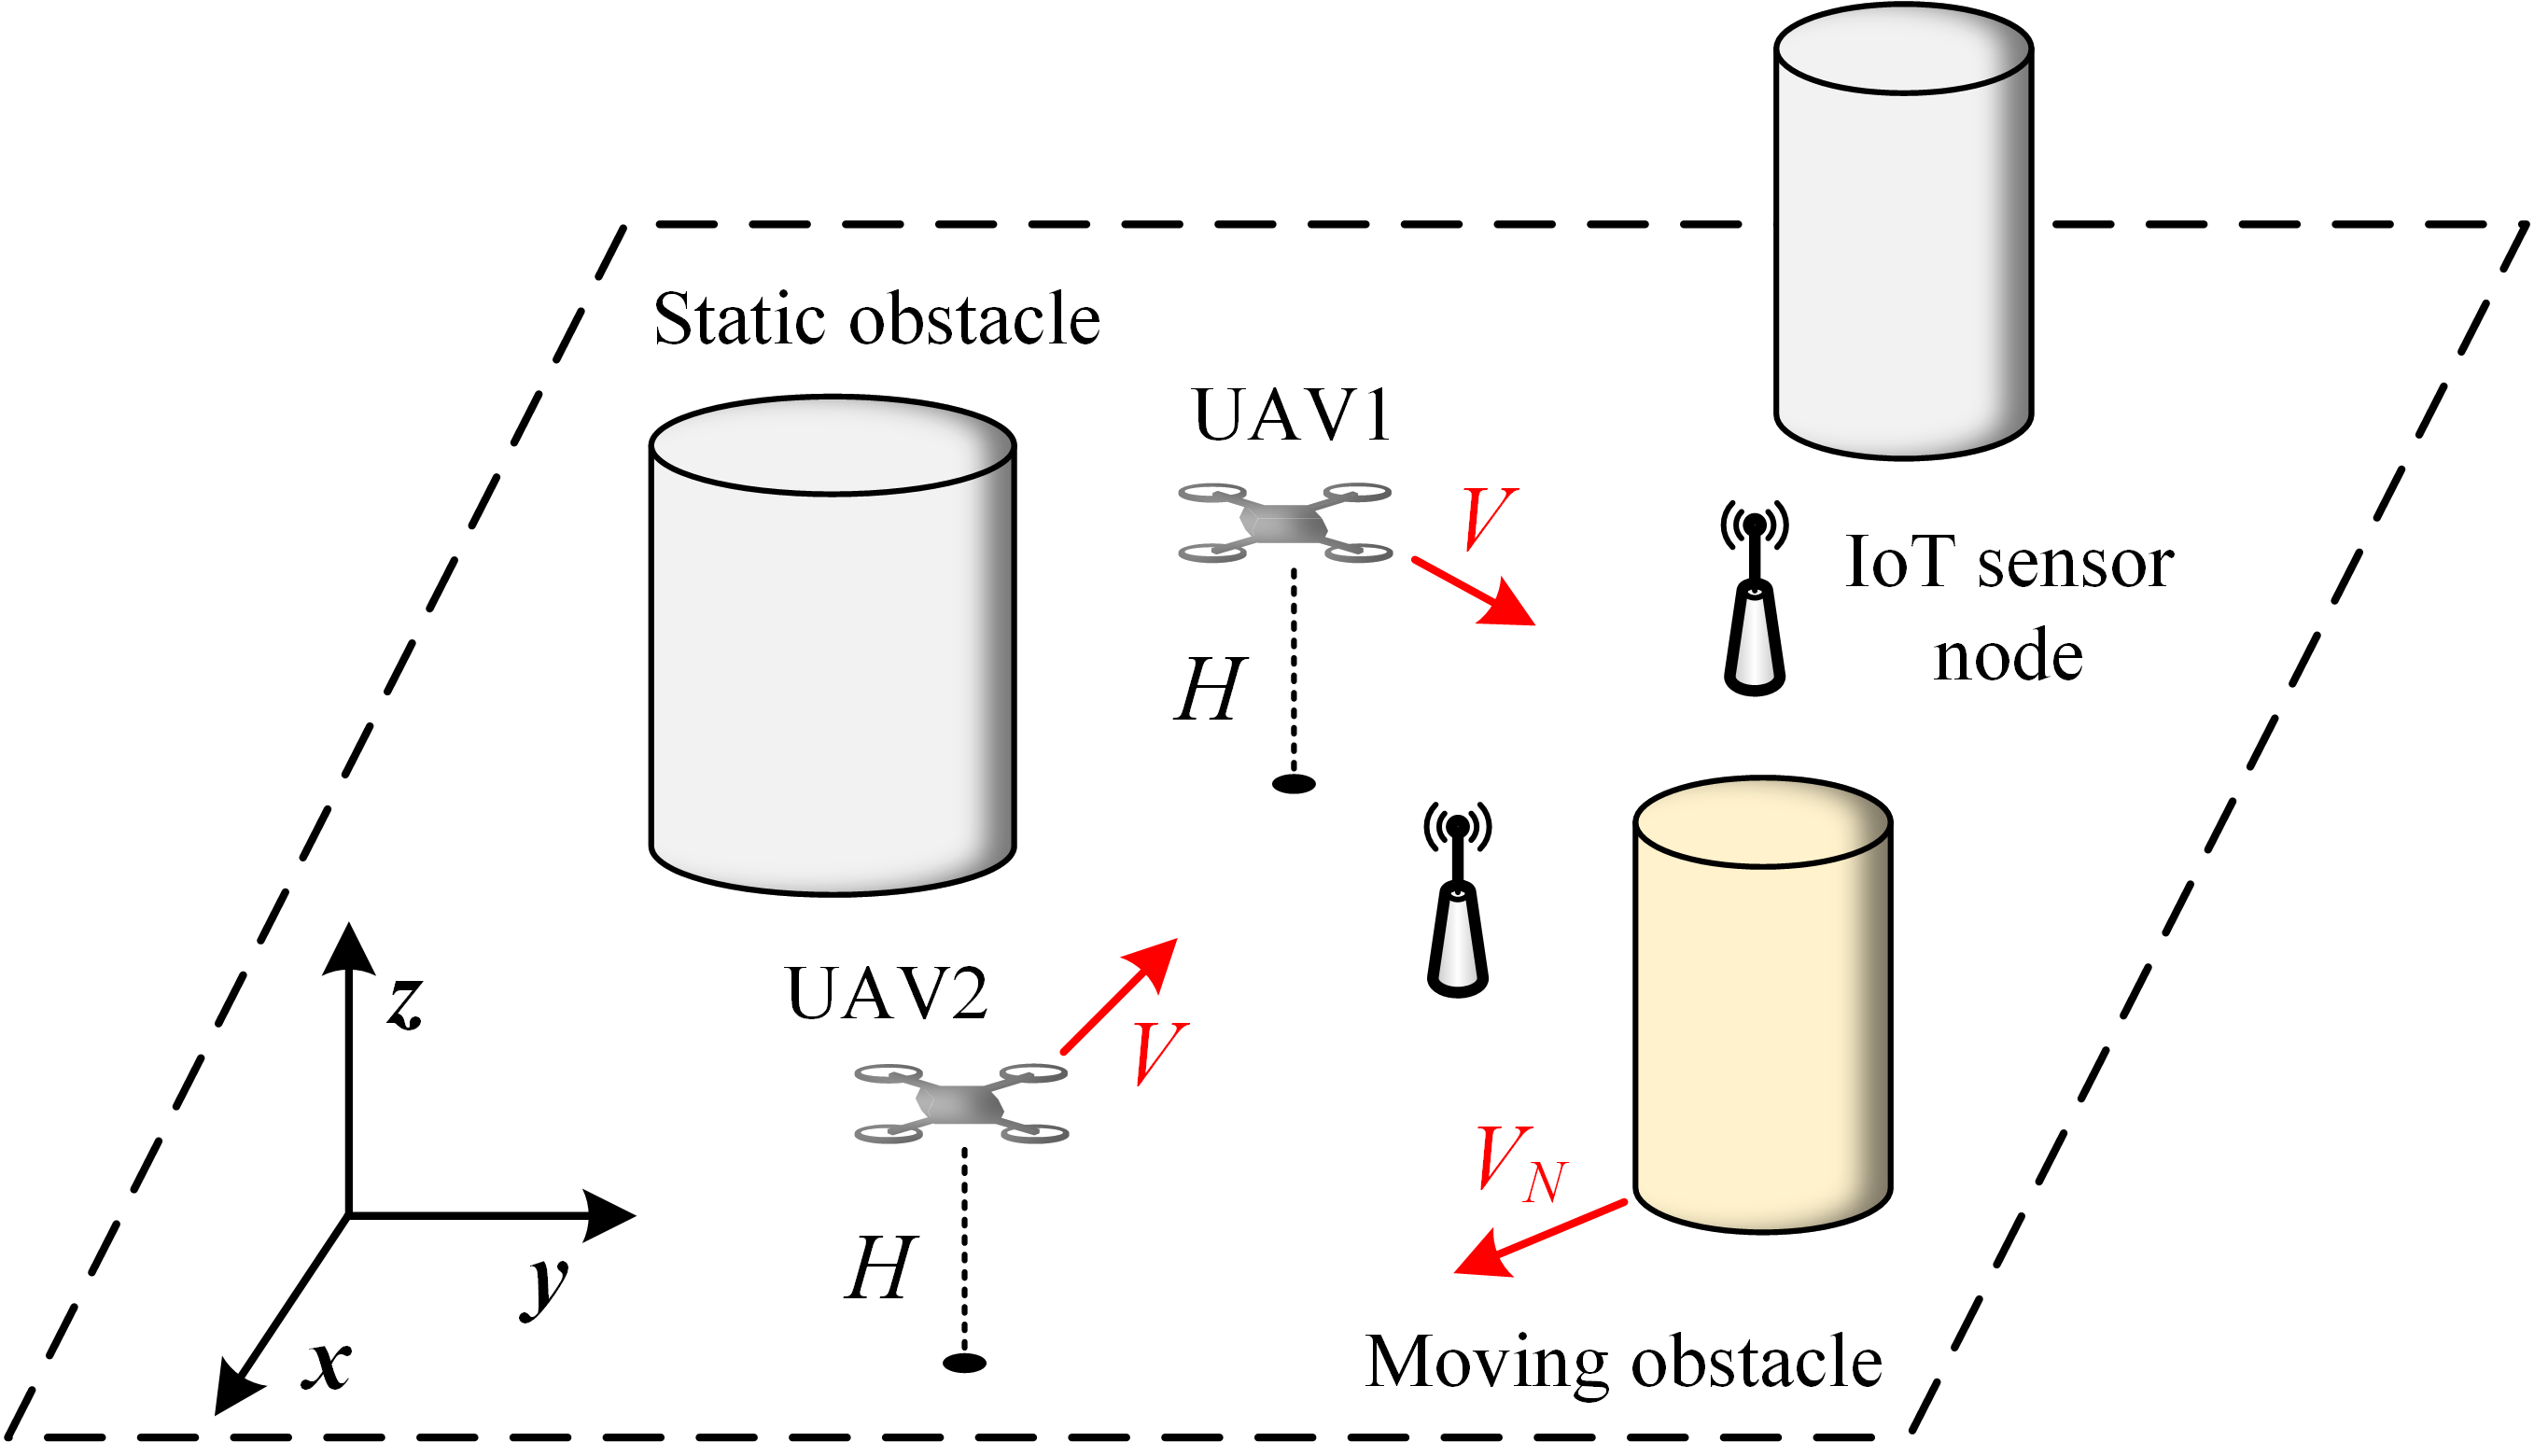
\includegraphics[width=0.48\textwidth]{fig/Env_Model.png}
%	\caption{The model of multi-UAV assisted data collection environment.\label{env_model}}
%\end{figure} 
\subsection{Communication model}\label{comm_model}
In the considered scene, the wireless signal propagation is attenuated in the environments with dense obstacles. The data transmission link refers to the statistical probability channel model \cite{MLi22}. In this model, line of sight (LoS) channel and non-line of sight (NLoS) channel occurs in probability distribution which is related to the elevation between UAV and IoT node. For the communication link between UAV $U_i$ and IoT node $I_j$, the probability of LOS channel is denoted as 
\begin{equation}\label{p_los}
  P_{LoS}^{i,j}=1/\left(1+\alpha e^{-\beta\left({\theta_{i,j}-\alpha}\right)}\right), 
\end{equation}
where $\theta_{i,j}$ is the angle of elevation between UAV $i$ and IoT node $j$ and $\alpha$, $\beta$ are the constance refer to the environment. Hence, the probability of NLOS link is $P_{NLoS}^{i,j}=1-P_{LoS}^{i,j}$. The path loss of communication link is denoted as 
\begin{equation}\label{path_loss}
\Lambda=
\begin{cases}
            K_0 \left({d_{i,j}/d_0}\right)^2 \mu_{LoS}, & \mbox{LoS link}\\
            K_0 \left({d_{i,j}/d_0}\right)^2 \mu_{NLoS}, & \mbox{NLoS link}
\end{cases}, 
\end{equation}
where $K_0=\left({4\pi f_c d_0 /c}\right)^2$, $f_c$ is the frequency of carrier, $c$ is the propagation velocity of light, $d_0$ is the reference distance, $d_{i,j}$ is the distance between $U_i$ and $I_j$, $\mu_{LoS}$ and $\mu_{NLoS}$ are the decaying factor corresponding to the LoS link and NLoS link. The signal transmission power of IoT node is $P_{I_j}$ and the reference distance $d_0$ is 1m. The path loss of the communication channel is regarded as the expectation in the occurence of LoS and NLoS, i.e. 
\begin{equation}\label{avg_path_loss}
  \bar{\Lambda}_{i,j}=K_0 d_{i,j}^2 \left(P_{LoS}^{i,j}\cdot\mu_{LoS}+P_{NLoS}^{i,j}\cdot\mu_{NLoS}\right).
\end{equation}
In this signal transmission model, the data rate for the transmission between $U_i$ and $I_j$ is denoted as 
\begin{equation}\label{data_rate}
  R_{i,j}=B\log_{2}\left(1+\frac{P_{I_j}}{\sigma^2 \bar{\Lambda}_{i,j}}\right),
\end{equation}
where $B$ is the bandwidth.

As the time interval of a data collection episode is divided into time slots, the set of time slots during the whole flight are denoted as $\mathcal{T}$. Data transmission starts when a UAV flies into the communication range of an IoT sensor node. The amount of data collected by UAV $U_i$ is denoted as 
\begin{equation}\label{collected_data}
  D_i=\sum_{I_j\in \mathcal{I}}{\sum_{t\in \mathcal{T}}{R^{i,j}_t \varphi^{i,j}_t \Delta T}},
\end{equation}
where $\Delta T$ is the time interval of each slot, $\varphi^{i,j}_t$ is the data transmission state of the channel between $U_i$ and $I_j$, where $\varphi^{i,j}_t=1$ signifies the $U_i$ resides within the communication range of $I_j$, while $\varphi^{i,j}_t=0$ corresponds to out-of-range conditions. 

%\subsection{Obstacle detection model}\label{obs_det}
%The mechanism of obstacle detection is based on the laser range finder. The range finder has 16 evenly distributed detection directions with maximum detection range $d_{\max}^{R}$. The range finder returns an array in which each value is the range to the surface of nearest obstacle in the corresponding direction. If the range finder detects no obstacle in a direction, the corresponding output value is $d_{\max}^{R}$. The output data of range finder is denoted as $\left\{d_{1}, d_{2}, ... , d_{16}\right\}$
%\begin{figure}[htbp]
%	\centering
%	%	\setlength{\abovecaptionskip}{-0.03cm}
%	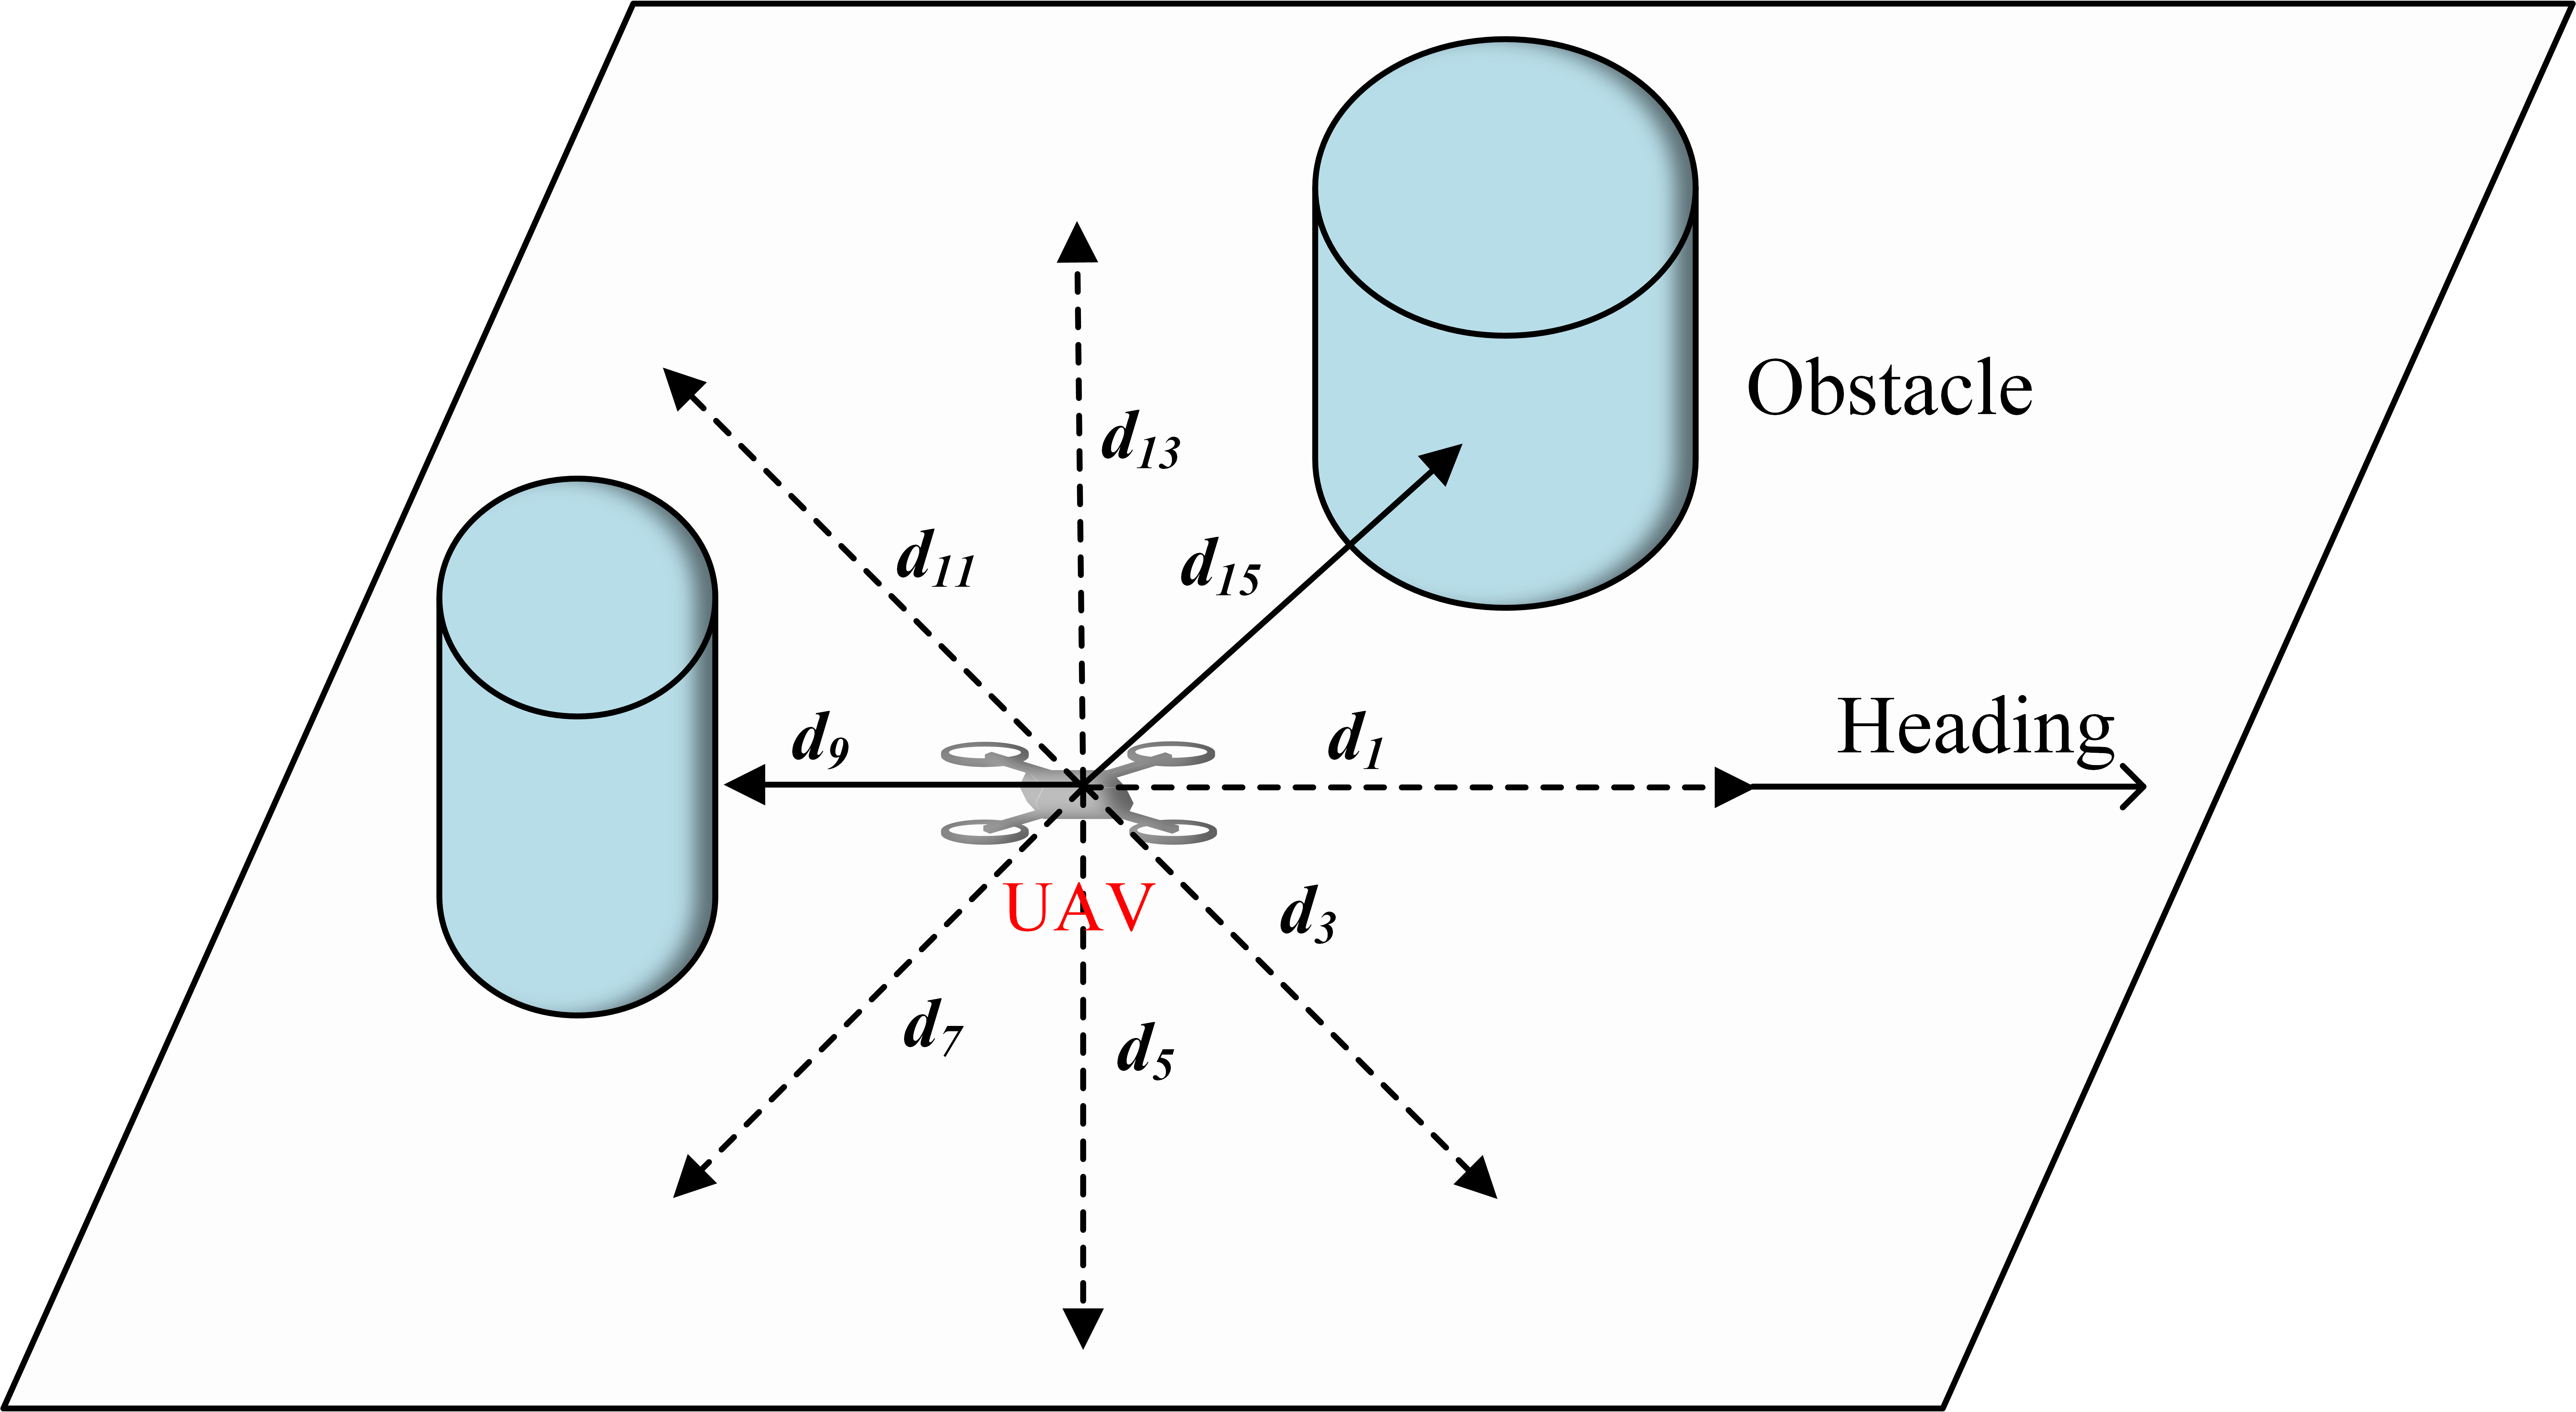
\includegraphics[width=0.45\textwidth]{fig/Obstacle detection.png}
%	\caption{The mechanism of obstacle detection. Note that the dash line arrow represents no detected obstacle in the corresponding direction, and the solid line arrow represents the distance to the detected obstacle. To make this figure concise, the arrows of some directions are omitted.}\label{obstacle_det}
%\end{figure}

\subsection{Optimization problem}\label{optimization_prob}
Based on the multi-UAV data collection system and communication model, the trajectory planning finds the optimal trajectories for UAVs to achieve the maximum collected data while using the least time, ensuring an efficient data collection system. 
%In this paper, the UAV trajectories are optimized to realize the minimum completion time and the maximum collected data while ensuring stable navigation in the environment that contains multiple UAVs and obstacles. 
%As the UAV makes decision at every time slot, the set of time slots during the whole flight are denoted as $\mathcal{T}$. The task completion time is the sum of time slot durations, i.e.
%\begin{equation}\label{path_len}
%  T=\sum_{t\in \mathcal{T}}{\Delta T}
%\end{equation}
%where $\Delta T$ is the duration of each time slot. The set of trajectories of UAVs is denoted as $\mathbf{P_U}$. 
%
%In data collection process, the data transmission starts when the UAV flies into the communication range $d_{\max}^{I}$. The data transmission state of $U_i$ and $I_j$ at time slot $t$ is denoted as: 
%\begin{equation}\label{data_collection_state}
%  \varphi^{i,j}_t=
%  \begin{cases}
%            1, & \mbox{$\lVert \mathbf{p}_t^{U_i}-\mathbf{p}^{I_j} \rVert < d_{\max}^{I}$}\\
%            0, & \mbox{$\lVert \mathbf{p}_t^{U_i}-\mathbf{p}^{I_j} \rVert > d_{\max}^{I}$}
%\end{cases}
%\end{equation}
%The collected data from all the IoT sensor nodes are denoted as: 
%\begin{equation}\label{collected_data}
%  D=\sum_{I_j\in \mathcal{I}}\sum_{U_i\in \mathcal{U}}{\sum_{t\in T}{R^{i,j}_t \varphi^{i,j}_t \Delta t}}
%\end{equation}
Under the condition of all UAVs successfully arrive at the destination, the amount of collected data is the sum of collected data amounts across the UAV swarm and the completion time is the time interval form departure of all the UAVs to arrival of the latest UAV. 
Hence, the trajectory planning problem on jointly optimizing the collected data amount and task completion time is denoted as 
\begin{align}
  P1:& \max\limits_{\mathbf{P_U}}\left({\omega_1 \sum_{U_i\in \mathcal{U}}{D_i}-\omega_2 \max_{U_i\in \mathcal{U}}T_i}\right)\label{optm_prob} \\
  s.t. \: & C1: d_{i,m} > d_{\min}^{B}, \forall U_i \in \mathcal{U}, \forall B_m \in \mathcal{B}, \nonumber \\
    & C2: d^{U}_{\min} < \lVert \mathbf{p}^{U,i}_t - \mathbf{p}^{U,k}_t \rVert < d^{U}_{\max} , U_i \neq U_k, \nonumber \\
  & C3: D_j\leq D^I_j,\: k\in\mathcal{I}, \nonumber
\end{align}
where $\omega_1$, $\omega_2$ are weighting coefficients, $T_i$ is the time interval from the departure of $U_i$ to its arrival, $d_{i,m}$ is the distance between UAV $U_i$ and obstacle $B_m$, $d_{\min}^{B}$ is the minimum distance to the obstacle surface for safety, $\mathbf{p}^{U_i}_t$ is the position of UAV in time slot $t$, $d^{U}_{\min}$ is the buffering distance for safety and $d^{U}_{\max}$ is the maximum communication maintaining distance between UAVs, $D_j$ is the collected data at IoT sensor node $I_j$, $D^I_j$ is the stored data at that node, the limitation $C1$ requests UAV to avoid collision with obstacles, $C2$ requests UAV to avoid collision with other UAVs while keep certain distance each other to maintain the air-to-air communication, $C3$ limits the collected data will not exceed the stored data. 

%\begin{figure}[htp]
%	\centering
%	%	\setlength{\abovecaptionskip}{-0.03cm}
%	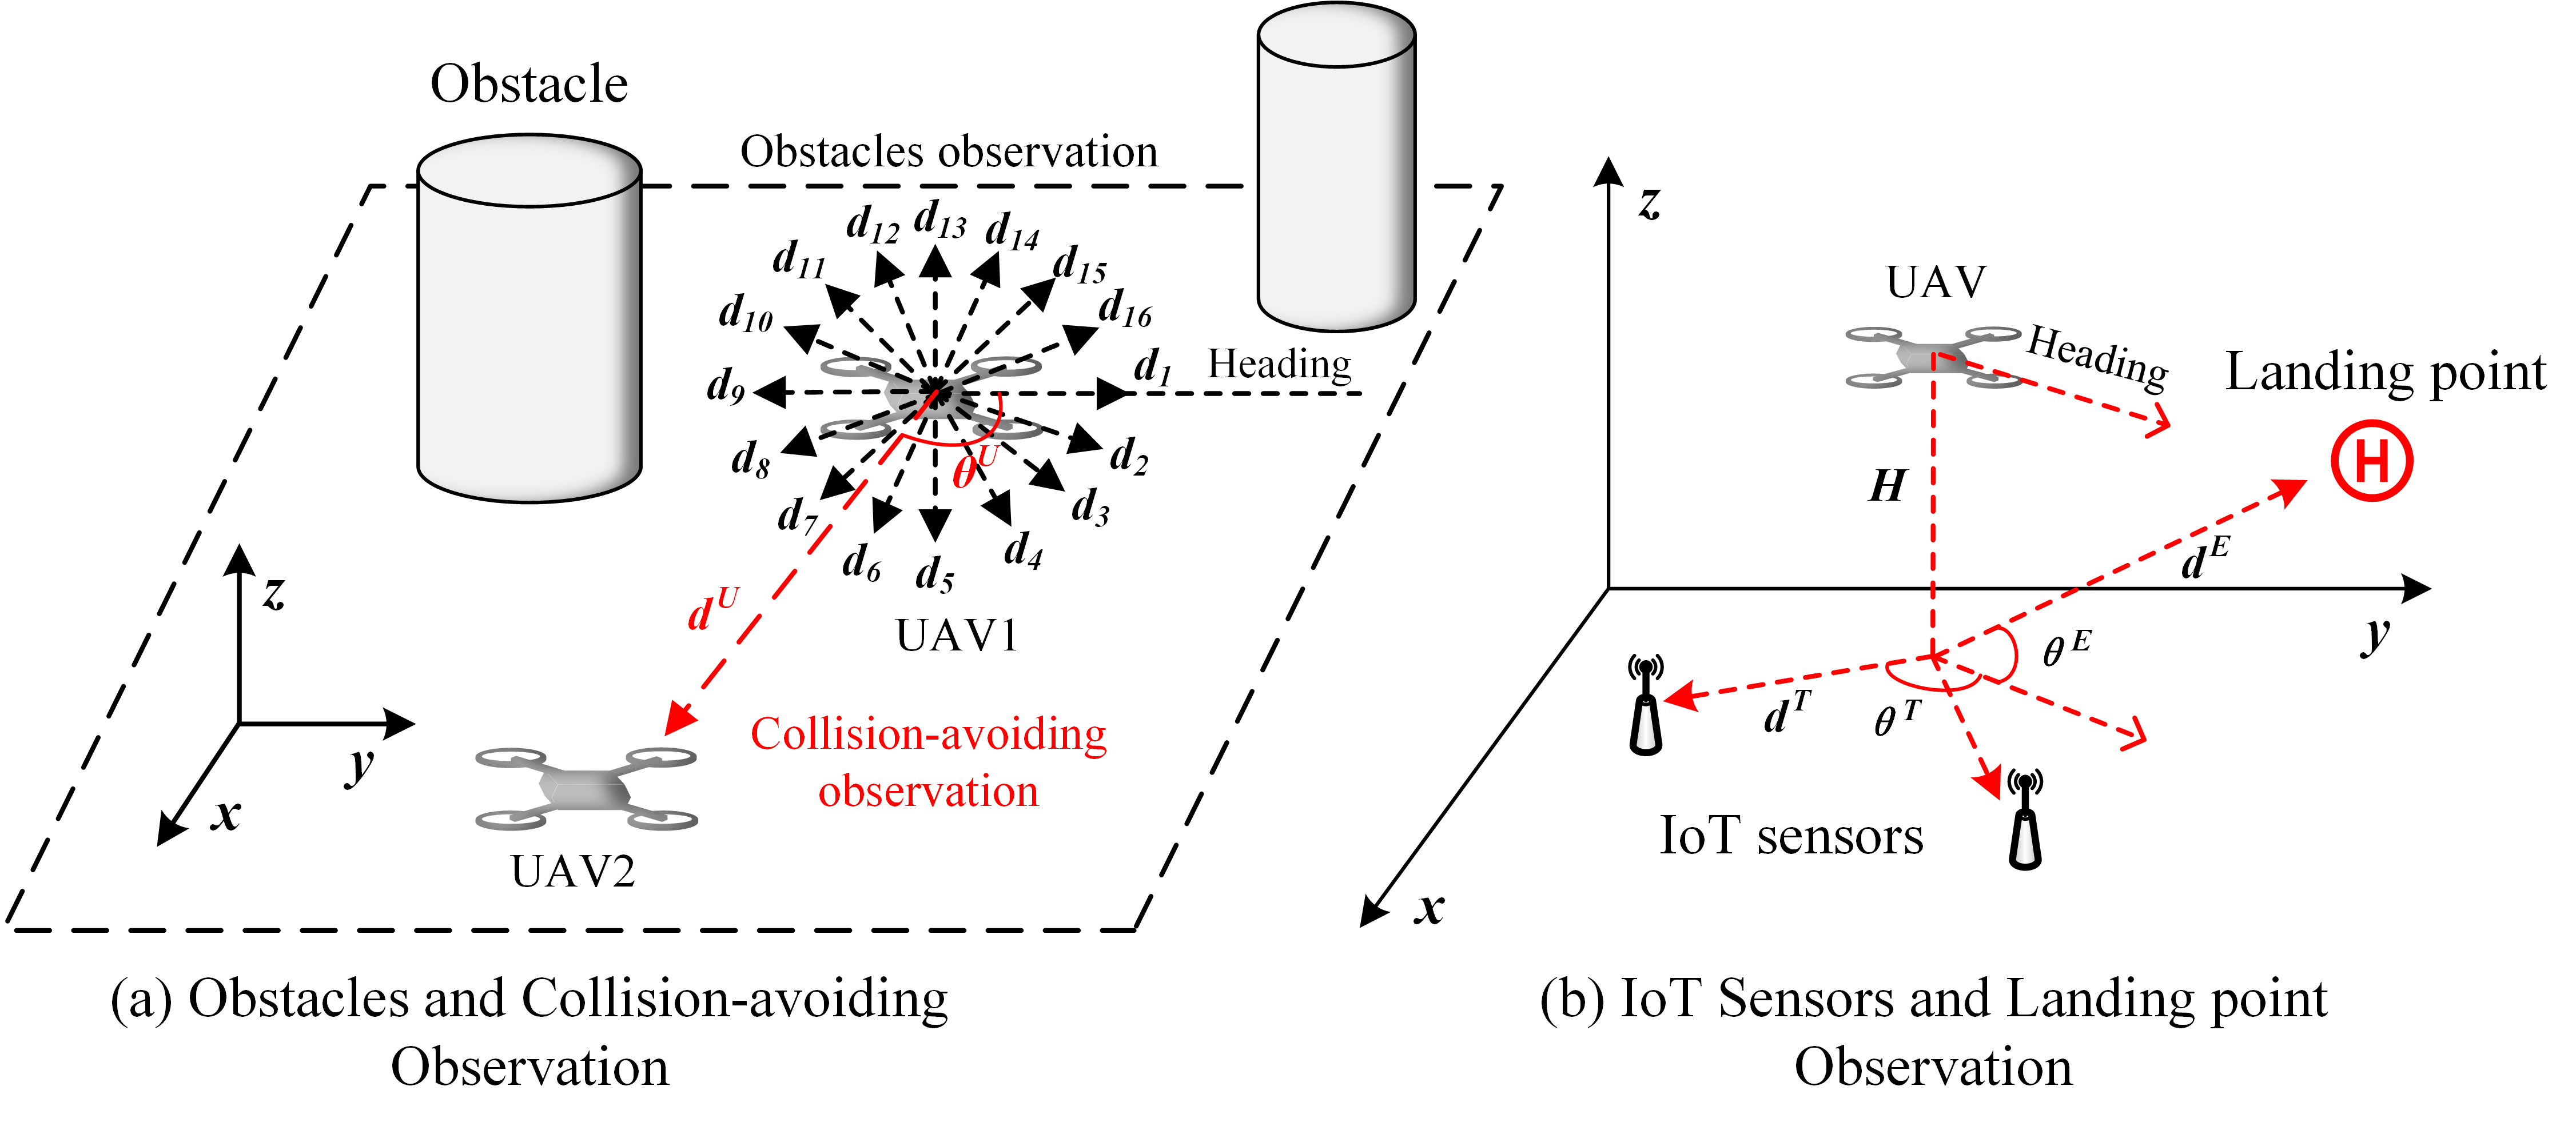
\includegraphics[width=0.48\textwidth]{fig/Obs.png}
%	\caption{The observation space of UAV for POMDP in the data collection environment: (a) Obstacle detection $o^{obs}$ and neighbour UAV observation $o^{uav}$; (b) IoT node observation $o^{node}$ and landing position observation $o^{tar}$ \label{observation}}
%\end{figure} 
%
%\begin{figure}[htp]
%	\centering
%	%	\setlength{\abovecaptionskip}{-0.03cm}
%	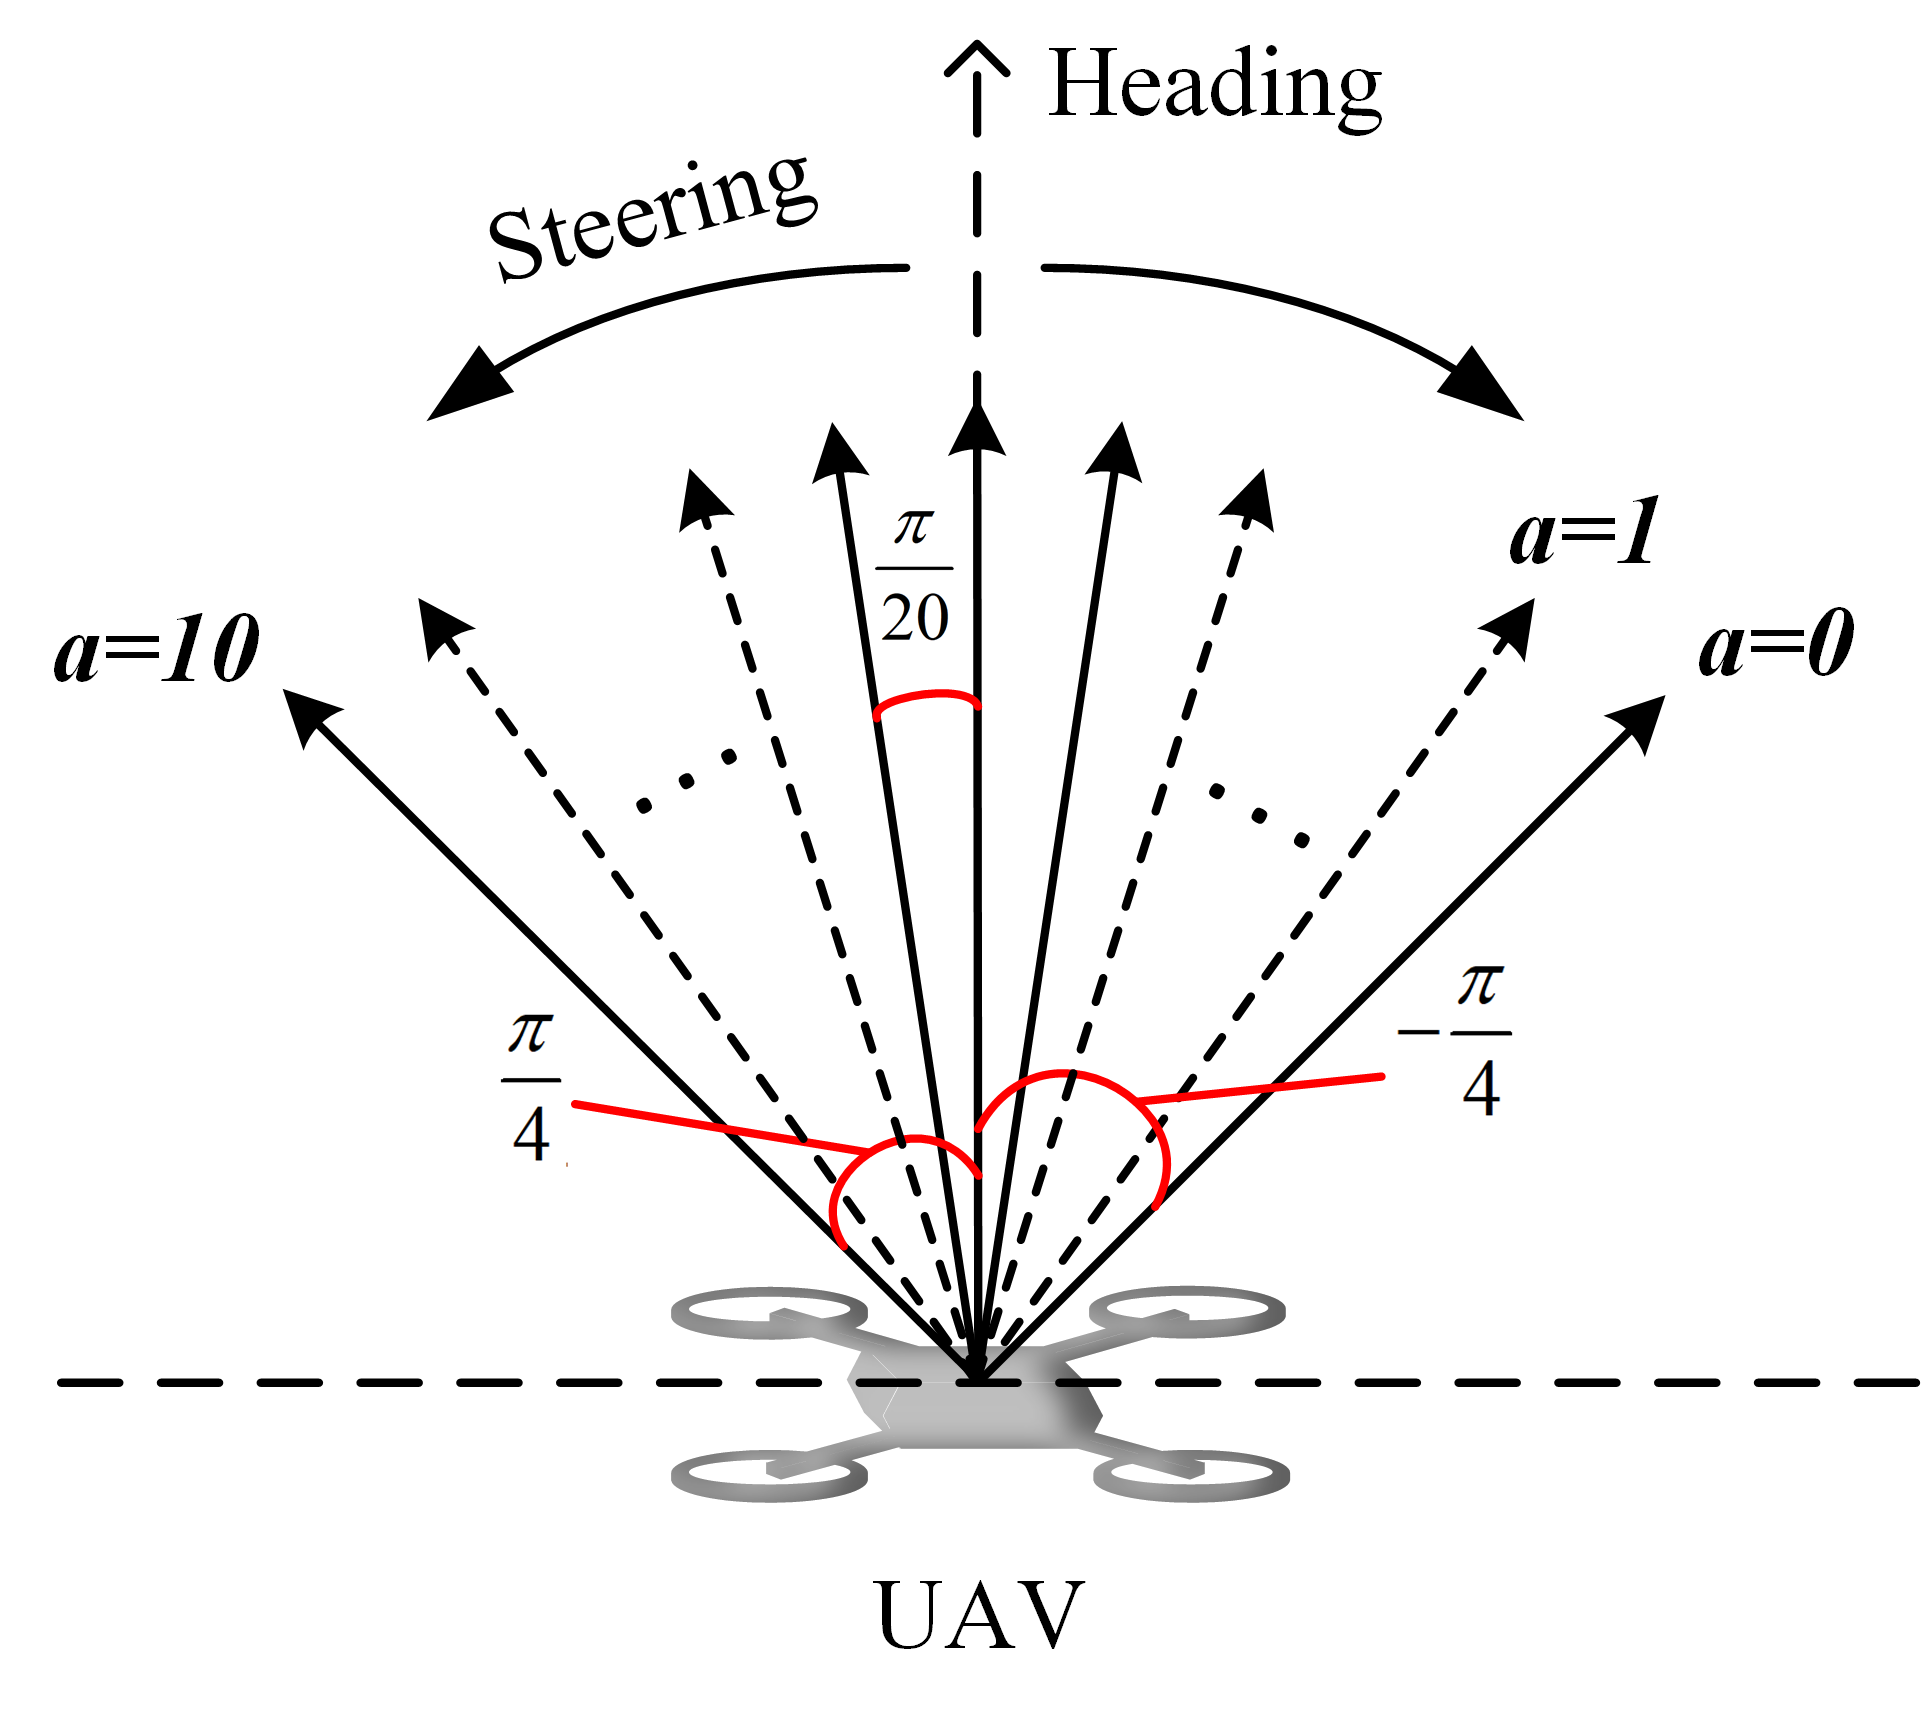
\includegraphics[width=0.32\textwidth]{fig/Action Space.png}
%	\caption{The definition of action space for POMDP \label{action_space}}
%\end{figure} 
\section{Methodology}\label{Method}
In this section, the cooperative DRL-based path planning algorithm for multi-UAV data collection is introduced. Firstly, the path planning is modelled as POMDP. Then, the cooperative multi-agent DRQN path control policy is described. Lastly, the fairness-oriented reward functions are designed. 

%\subsection{Node searching-based path planning}\label{data_collection}
%As the environment is unknown for UAVs, in this work, each UAV use the IoT sensor node detecting sensor with limited detection range to obtain the positions and data amounts of IoT sensor nodes, which is shown in Fig. \ref{fig_dc}. Then it plan an optimal path to the communication regions of IoT nodes based on these information. Besides, for collaboration, each UAV obtains the information includes UAV position and discovered IoT sensor nodes form adjacent UAVs. The IoT node detection region is changing with the UAV movement and the path planning updates based on realtime information of discovered IoT sensor nodes. During the flight, the UAV obtain the position of destination and the data from range finders to keep the movement toward to the destination and avoid the obstacles. The UAV plans its flying path dynamically until it reaches the destination. 
%\begin{figure}[htbp]
%	\centering
%	%	\setlength{\abovecaptionskip}{-0.03cm}
%	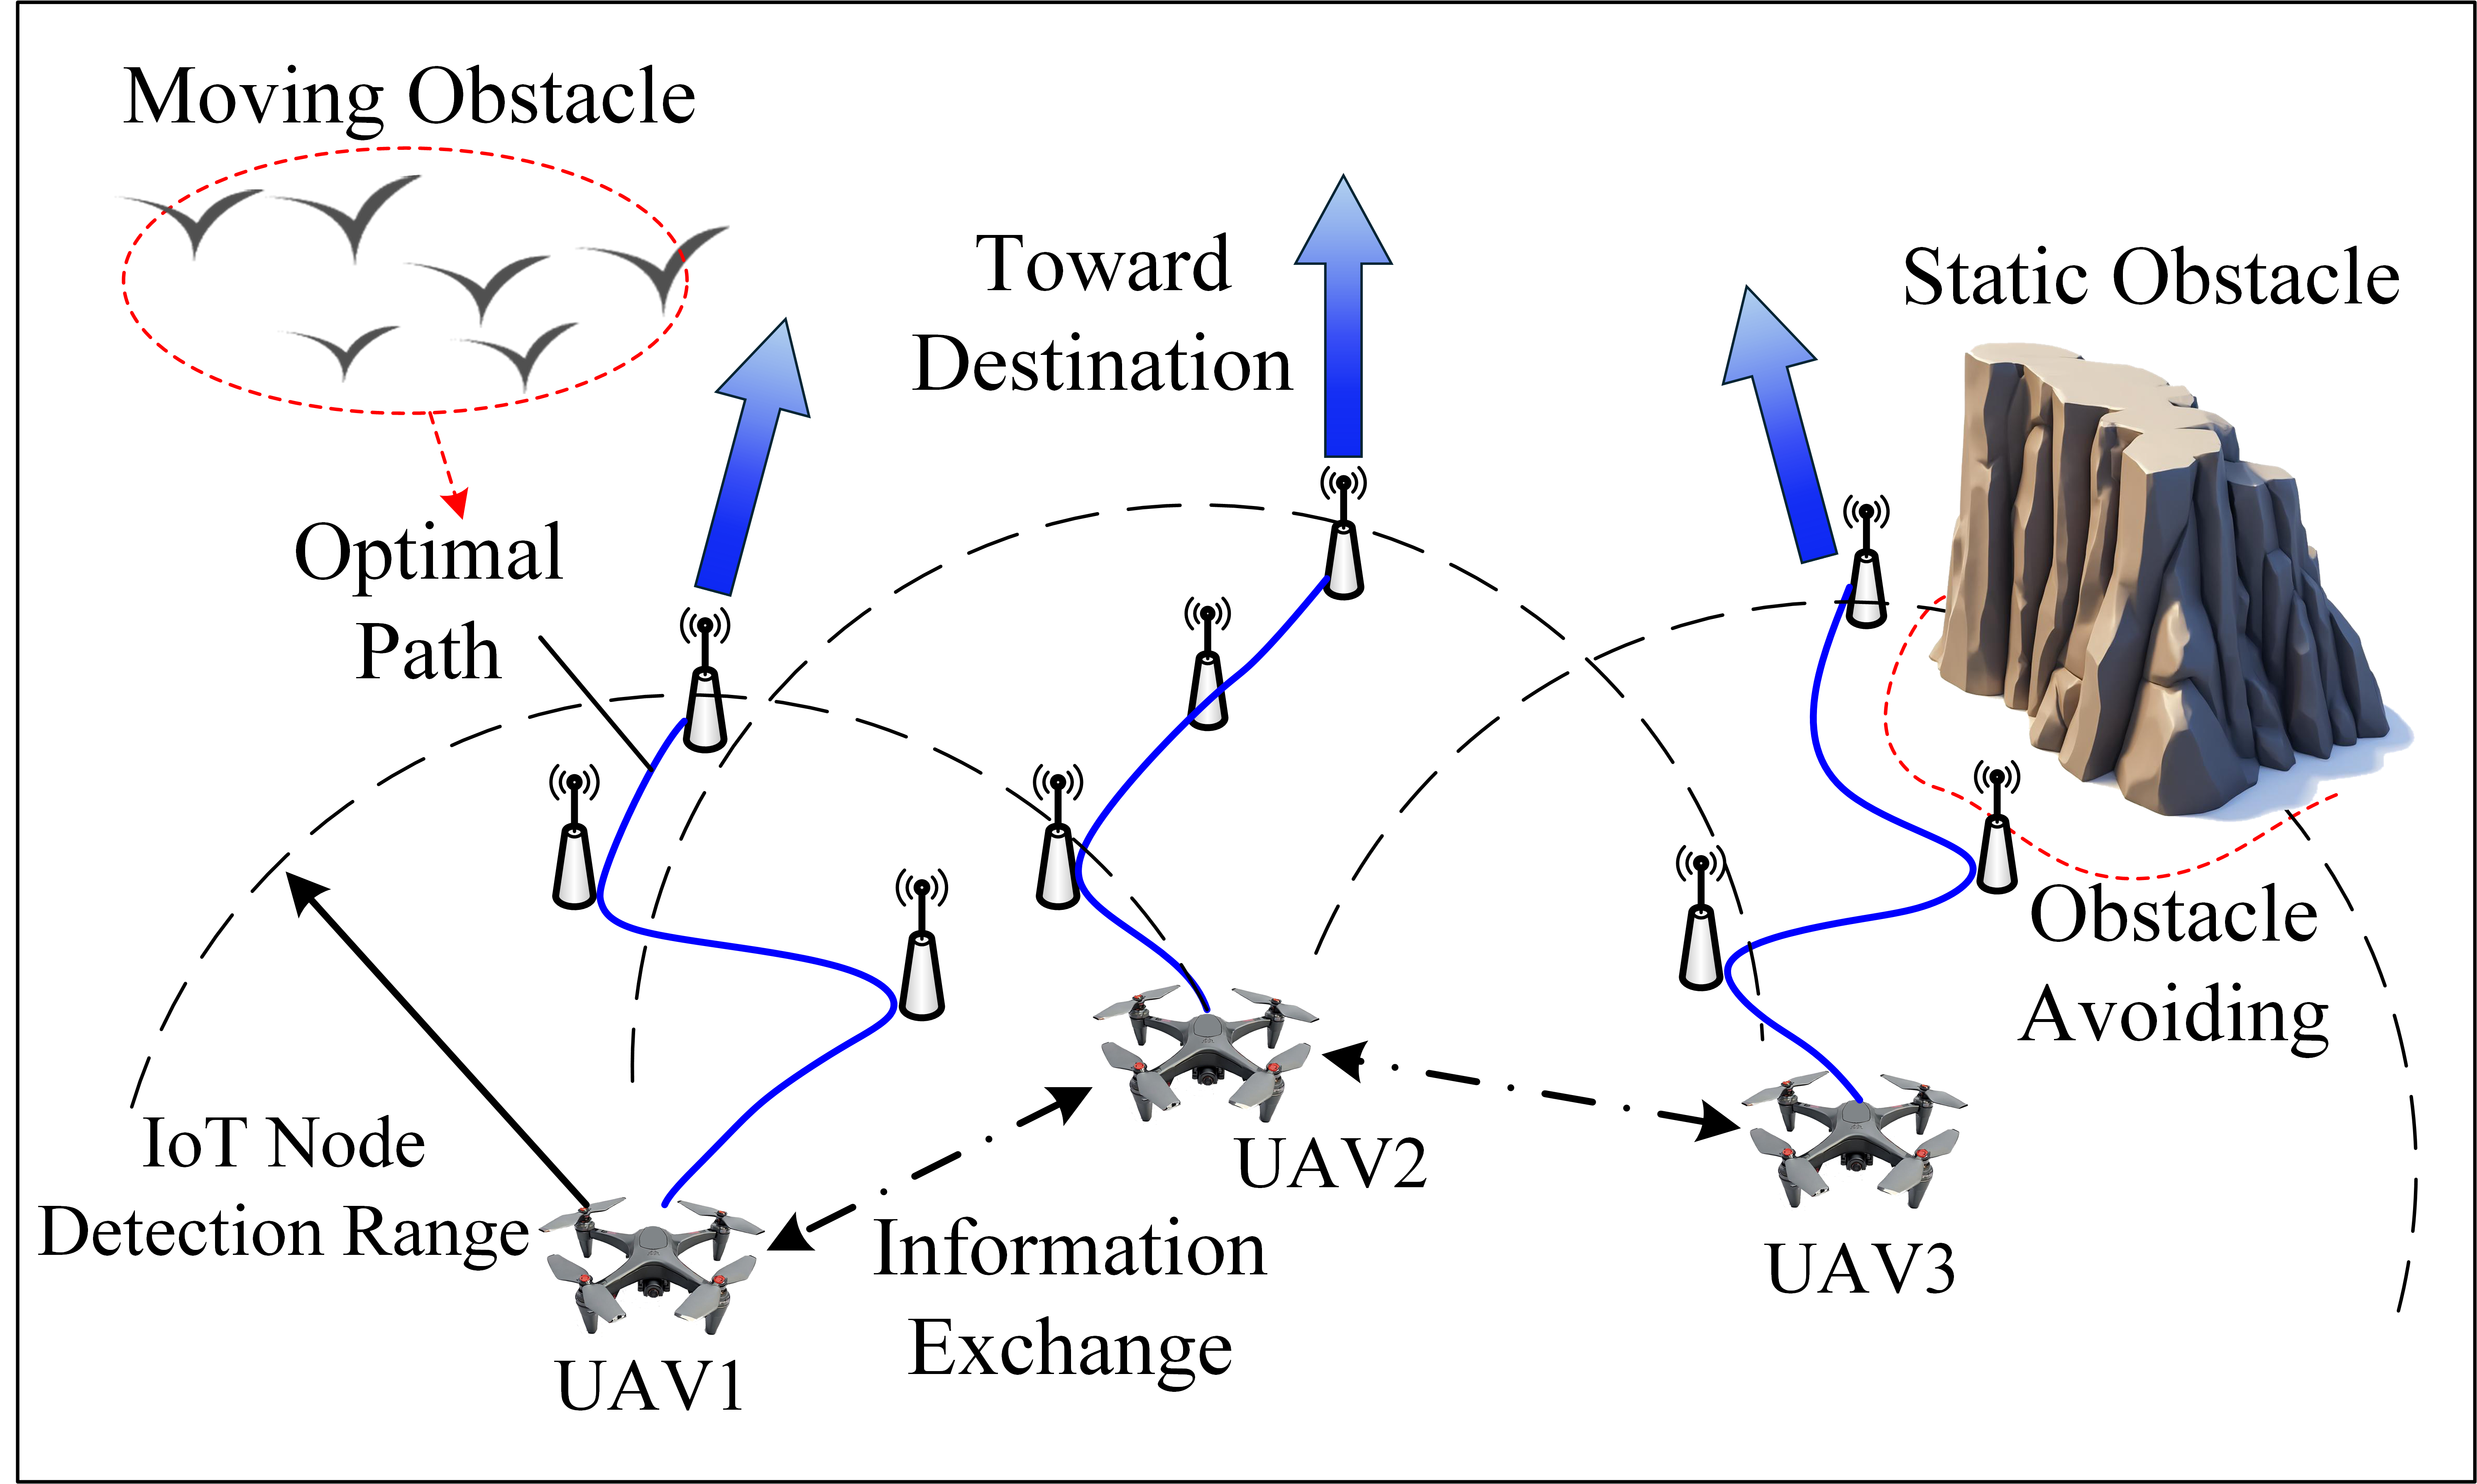
\includegraphics[width=0.4\textwidth]{fig/Data Collection.png}
%	\caption{The schematic diagram of POMDP-based data collection trajectory planning model. }\label{fig_dc}
%\end{figure}
%Our design of data collection mechanism contains two parts: one is target point indication, the other is IoT nodes collection array. The data collection task region is assumed that evenly distributes target points. As shown in Fig.\ref{collection_allocation}, the region is divided into several sections along the flying direction. The edge of each section has the target point for UAV navigation. While UAV is flying toward the target point, the UAV searches the IoT nodes and collects the data. After all data from discovered IoT nodes are collected and UAV approaches the edge of the current section, the collection process goes to next stage and the UAV is navigated to the next target point. For the target point navigation, UAV obtains the distance and direction to the target point according to the positions of UAV and target point, i.e. 
%\begin{equation}\label{target_observation}
%  o^{tar}=\left(d_{tar}, \theta_{tar}\right),
%\end{equation}
%where $d_{tar}$ is the distance to the target point, $\theta_{tar}$ is the direction angle to the target point. 
%
%The UAV keeps searching for the IoT nodes during its flight with detection range $d_{max}^{node}$. When the $i$th node is in the detection range of UAV, the connection is established and UAV obtains the information about the $i$th IoT node which is denoted as
%\begin{equation}\label{node_observation}
%  o^{node}_{i}=\left(n^{node}_{i},d^{node}_{i},\theta^{node}_{i},D^{node}_{i}\right),
%\end{equation}
%where $n^{node}_{i}$ is the identical number of the node, $d^{node}_{i}$ is the distance to the node, $\theta^{node}_{i}$ is the direction to the node, and $D^{node}_{i}$ is the data size of the node in bytes. In each UAV, an array stores the information of discovered IoT nodes sorted by the distance between UAV and node. If one node is discovered by two UAVs in the same time, UAVs will communicate each other to compare the distance cost for data collection of that node. The UAV that has more cost will give up the data collection. The IoT node searching array which has the capability of 5 nodes is denoted as 
%\begin{equation}\label{node_array}
%  o^{node}=\left(o^{node}_{1}, o^{node}_{2}, ... , o^{node}_{5}\right).
%\end{equation}
%When UAV has searched IoT nodes, it will fly into the communication ranges of nodes to collect data. The collection sequence and trajectory will be decided jointly by its DRL-based algorithm. 
%\begin{figure}[htbp]
%	\centering
%	%	\setlength{\abovecaptionskip}{-0.03cm}
%	\includegraphics[width=0.45\textwidth]{fig/Collection Allocation.png}
%	\caption{The mechanism of data collection.}\label{collection_allocation}
%\end{figure}
\subsection{Modeling UAV data collection as an POMDP} \label{sec_pomdp}

The trajectory planning in complex and dynamic environments faces these challenges: (1) The environment is complex and partially observable. UAVs rely solely on the localized sensory data due to their airborne sensors with limited perception capabilities. (2) The environment is dynamically changing due to the present of moving obstacles like bird flocks and the concurrent multi-UAV operations. UAVs necessitate flexible replanning to address the dynamics of environment. 
Hence, the trajectory planning is modelled as POMDP where a trajectory planning is composed of sequential trajectory control decision-makings. UAVs are modelled as agents and make each trajectory control decision by the real-time perception of environment and UAV swarm. The POMDP design is described as follows: 
%\textit{a) Agents $\mathcal{N}$}: In our multi-agent path planning solution, each UAV is regarded as an agent. All the agents make their respective path decisions simultaneously in the same environment and receive their respective rewards. The agents are denoted as $\mathcal{N}=\left\{N_1,N_2,\cdots,N_U\right\}$ where $U$ is the number of UAVs. 

\textit{(a) State:} State is the current parameters of all the objects in the environment as data collection episode be in progress. In this POMDP, the state contains the positions of all the UAVs, IoT sensor nodes and obstacles, and the data amounts in IoT sensor nodes. 

\textit{(b) Observation:} Agents obtain the observations form the current state for input of trajectory planner. The set of observations is denoted as $\mathcal{O}=\left\{o_1, o_2, \cdots, o_N\right\}$. For effective data collection, each UAV observes the state information of destination, IoT sensor nodes, obstacles and adjacent UAVs. 
\begin{itemize}
  \item To navigate to destination, the observation of destination is denoted as $o_{T}=\left(d_{T}, \theta_{T}\right)$, where $d_{T}$ is the distance to the target point, $\theta_{T}$ is the direction angle to the target point.
  \item To find a path to the IoT sensor nodes with high collection efficiency, the observation of the state of IoT sensor nodes is denoted as $o_{I}=\left\{\left(d^{I}_{1},\theta^{I}_{1},D^{I}_{1}\right),\left(d^{I}_{2},\theta^{I}_{2},D^{I}_{2}\right),\cdots,\left(d^{I}_{5},\theta^{I}_{5},D^{I}_{5}\right)\right\}$, where $d^{I}_{i}$ is the distance to the node, $\theta^{I}_{i}$ is the direction to the node, and $D^{I}_{i}$ is the data size of the node in bytes.
  \item To avoid collisions to the obstacles in the environment, the agent observes the distance to the surface of obstacle by the mechanism of range finder, i.e. $o_{B}=\left(d^{B}_{1}, d^{B}_{2}, \cdots , d^{B}_{16}\right)$, where each element of this array is the distance to the surface of obstacle in one direction. 
  \item To keep distance to adjacent UAVs and avoid any conflict, the observation of two nearest adjacent UAVs is denoted as $o_{U}=\left\{\left(d_{1}^{U}, \theta_{1}^{U}\right), \left(d_{2}^{U}, \theta_{2}^{U}\right)\right\}$, where $d_{U}$ is the distance to an adjacent UAV, $\theta_{U}$ is the direction to an adjacent UAV. 
\end{itemize}
The combination of these component is local observation that is denoted as $o_{l}=\left({o_{T},o_{I},o_{B},o_{U}}\right)$. 
\begin{itemize}
  \item For collaboration on data collection, each UAV agent exchange its IoT sensor node observation with the two nearest adjacent UAVs. The obtained observation from adjacent UAVs is denoted as $o_{a}=\left(o^{I}_{a,1},o^{I}_{a,2}\right)$. 
\end{itemize}
Consequently, the observation $o$ is denoted as 
\begin{equation}\label{obs}
  o=\left({o_{l},o_{a}}\right). 
\end{equation}

\textit{(c) Action:} All the agents select and execute actions simultaneously. The set of actions is denoted as $\mathcal{A}=\left\{a_1, a_2, \cdots, a_N\right\}$. The action of each agent is its steering angle. 
%Refer to the motion model of UAV, the action space should be continuous. Although continuous action space can realize more precise trajectory planning than discrete action space, the trajectory planner with continuous action output is more complex. 
For the considerations of both computing efficiency and trajectory planning precision, a discrete action space is designed by sampling the continuous space of steering angle. The action space contains 11 integer scalers values from 0 to 10, corresponding to the steering angles that evenly sampled from $-\pi/4$ to $\pi/4$. The negative value of steering angle means right steering and the positive value means left steering. The step size of steering angle in action space is $\pi/20$. 

%\textit{d) Reward function $\mathcal{R}$}: When the agent takes action $a$ at state $s$, the agent receive the reward $r$ as a feedback on the fitness of optimization goal, i.e. $\mathcal{R}:\mathcal{S}\times\mathcal{A}\rightarrow\mathbb{R}$. According to the design of observation space, the agent use observation that relevant to the state of local surrounding environment for action decision, which can easily stuck in local optimal learning result. The reward shaping to dense reward function avoids the local optimum and increases the learning efficiency\cite{Miranda24}. To realize the optimization goals, we design a multi-objective dense reward function which is described in the following. For the decentralized RL structure, each agent receives its reward independently, i.e. $r_i=\mathcal{R}\left(s, a_i\right), i\in\mathcal{N}$.

%\textit{e) State transition function $\mathcal{P}$}: After all the agents conduct action at state $s$, the environment will change to next state $s'$ by the state transition function, i.e. $\mathcal{P}:\mathcal{S}\times\mathcal{A}\rightarrow\mathcal{S}'$. State transition function reflects the operation of system model. For our model-free algorithm, it is unnecessary for agents to know the state transition function. 

%At every time slot of action decision, the agent choose an action based its observation $o$ by its policy which is denoted as
%\begin{equation}\label{act_policy}
%  a=\pi\left({o}\right).
%\end{equation}
%In policy $\pi$, the action choice is evaluated by value $Q$ which is the expectation of the reward that agent will receive in the future. 
%\begin{equation}\label{q_func}
%  Q_{\pi}\left({o,a}\right)=\mathbb{E}_{\pi}\left[\sum_{k=0}^{\infty}{\gamma^{k}r_{t+k+1}\left|o,a\right.}\right]
%\end{equation}
%where $\gamma$ is the discount factor in $\left[{0,1}\right]$, $r_{t}$ is the reward that the agent obtained at time $t$. The action choosing value $Q_{\pi}\left({o,a}\right)$ is to estimate the future reward agent can gain after make the action choice $a$ at observation $o$. 
%To realize the function of path planing, our work is to solve the policy $\pi$ by DRL. 

\subsection{Dual-channel trajectory control policy}\label{policy}

\begin{figure*}[htb]
    \centering
    %	\setlength{\abovecaptionskip}{-0.03cm}
    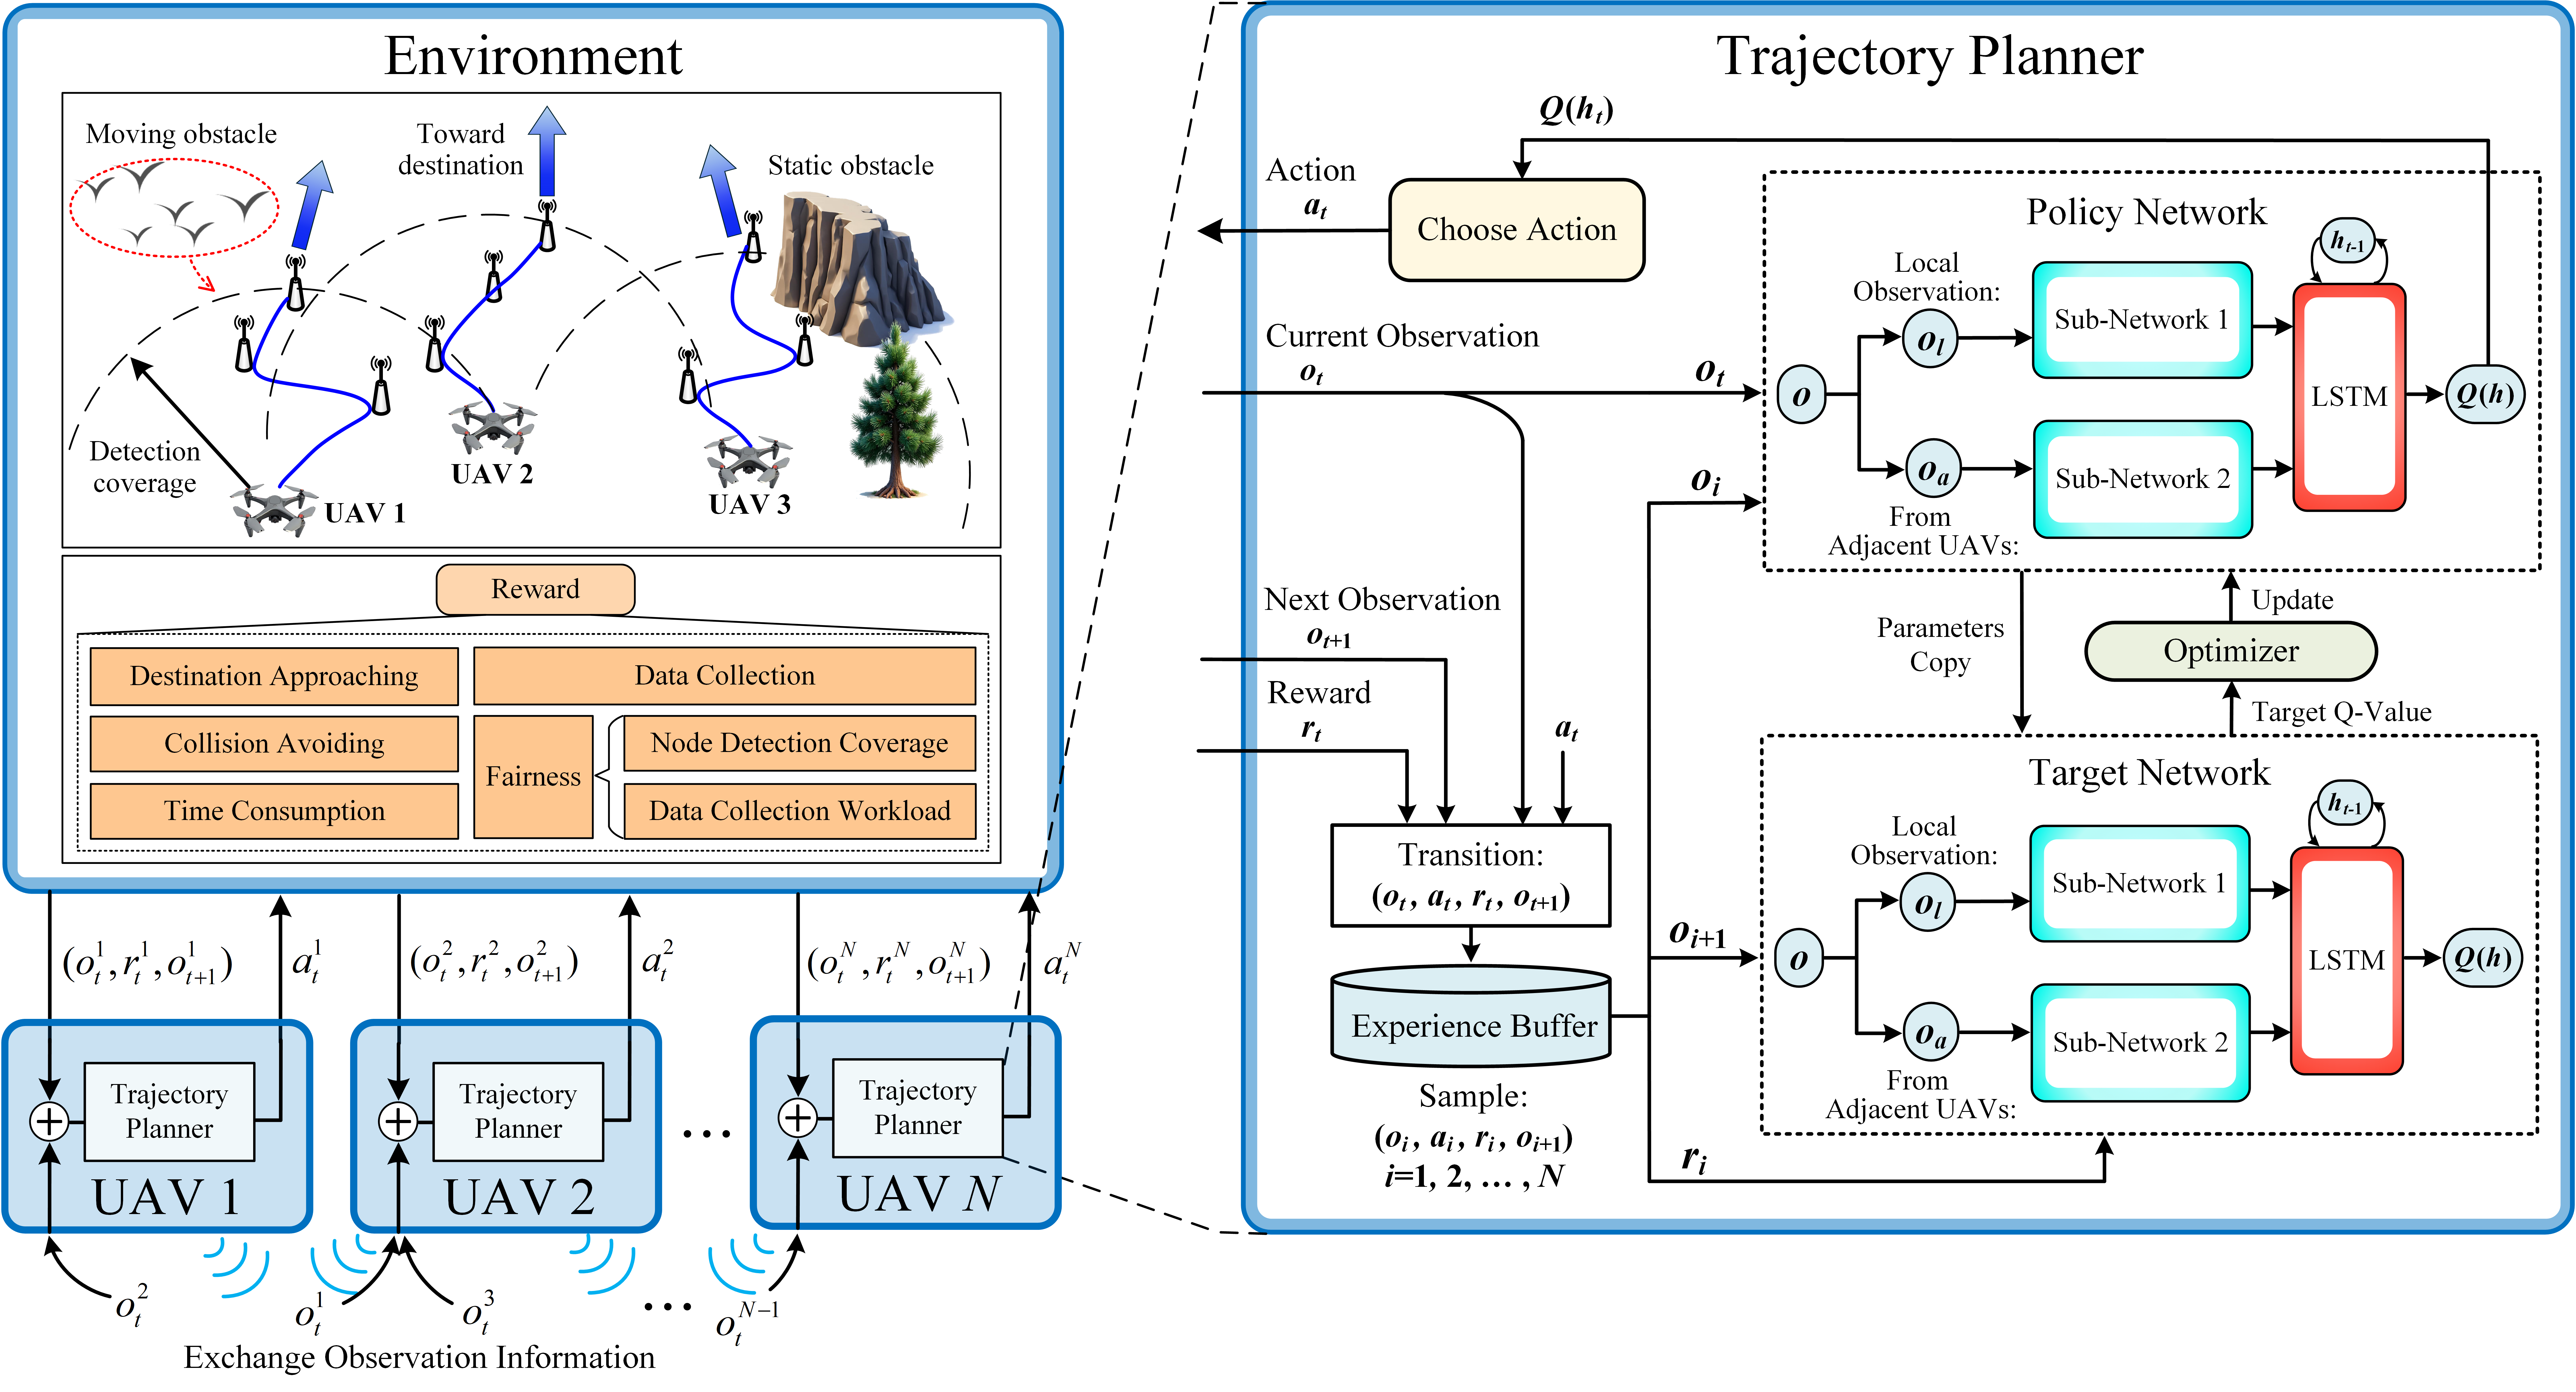
\includegraphics[width=0.9\textwidth]{fig/Framework_new.png}
    \caption{The structure of proposed DRQN-based algorithm for path planning.}\label{framework}
\end{figure*}

During a data collection episode, at each step, each UAV agent select an action based on the observation by its intelligent trajectory control policy. In this paper, a deep recurrent Q-network (DRQN)-based trajectory control policy is proposed. Firstly, a deep neural network (DNN) is decomposed into two sub-networks to extract the features of local observation and observations form adjacent UAVs separately. Then, a long short term memory (LSTM) is utilized to aggregate the features of historical inputs. Lastly, a output layer computes the values of action choices based on the aggregated features. As the optimal policy, the agent choose and execute the action that has the highest estimated value. 
%Q-learning is a value-based reinforcement learning algorithm in which the agent use state-action value function $Q_{\pi}\left({o,a}\right)$ to make its action decision. In this paper, we use DRQN algorithm that use neural networks to approximate the value function to make flying path decision based on the observation input. Compared to Q-learning, DQN can handle the continuous state space and occupies less memory space. Because of range finder-based obstacle detection and the mechanism of data collection, the UAV cannot obtain the full state such as the positions of all the obstacles and the states of all the IoT nodes, which is disadvantageous in complex environment. A LSTM layer is deployed into the neural network to store the previous observations. This memory contains more information about the environment state than the observation in single time slot. 
%Traditional Q-learning algorithm use a table to store the value function $Q_{\pi}\left({s,a}\right)$. However, in UAV-assisted data collection model, the massive combinations of state and action $\left({s,a}\right)$ makes the table based value function is hard to be stored. Deep Q-learning network (DQN) algorithm use neural networks to approximate the value function. Compared to Q-learning, DQN can handle the continuous state space and occupies less memory space. In this work, the path planing for UAV-assisted data collection is modeled as POMDP. As equation (\ref{ht_func}) illustrates, the agent consider the trajectory of history observations as the current state. Long short term memory (LSTM) is introduced to memory the history observations. The DQN comes to deep recurrent Q-learning network (DRQN). 

Traditional Q-network-based DRL algorithms use single deep neural network to process the input information. As the obtained observation of each UAV contains both information of local environment and exchanged observations from adjacent UAVs, processing this high dimensional information requires a deep neural network with a large number of neurons. Hence, in the first stage of feature extraction, the two observation components $o^l_t$ and $o^a_t$ are processed by a twin of deep neural networks separately. Each processing channel has lower input dimension. As shown in Fig. \ref{framework}, in policy network of agent $U_i$, a twin of decomposed deep neural networks are deployed to extract the features from local observation $o^l_t$ and observations from adjacent UAVs $o^a_t$. The respective extracted feature vectors $\phi^{i,l}_t$, $\phi^{i,a}_t$ are generated. By using dual sub-networks, the agent establishes situational awareness of both the environment and the adjacent agents with low computational complexity. 

Then, the feature vectors are concatenated at the input port of the LSTM layer. 
%\begin{equation}\label{LSTM_i}
%  x^{L,i}_t=\left({\phi^{i,l}_t,\phi^{i,l}_t}\right).
%\end{equation}
%As shown in Fig. \ref{framework}, the architecture of DRQN contains the policy network $\theta_{Q}$ and target network $\theta_{Q}'$. The target network is used for path planning action making. At each time slot, the agent input the observation to policy network and get the values of all the action choices. Then it choose the action that is predicted to has the highest value, i.e. 
%\begin{equation}\label{choose_action}
%  a_t=\arg\max\limits{a}{Q_{\pi}\left({o_{t},a}\right)},
%\end{equation}
%where $o_t$ is the observation at time slot $t$ and $a_t$ is the action choice at this time slot. 
The LSTM achieves the processing of concatenated features of local observation and adjacent UAV observations and aggregation the historical observations. Based on the fundamental function of deep neural network, each neuron in LSTM selectively store the input information into its memory cell and remove the irrelevant memory by its gate functions that include forget gate, input gate and output gate. The forward function of LSTM processes the current observation, the previous output and the memory to establish $h^i_{t}$ that is a feature vector about the historical environmental information, i.e. 
\begin{equation}\label{lstm_fwd}
  h^i_t=f^i_L\left[{\left({\phi^{i,l}_t, \phi^{i,a}_t}\right), h^i_{t-1}}\right],
\end{equation}
where $f^i_L$ is the forward function, $h^i_{t-1}$ is the previous output and $h^i_t$ is the current output. As the environmental perception based on observation is localized due to the partial observability of environment, by aggregating historical observations, the scope of environmental perception is expanded. With the aggregated features, UAV agents holistically comprehend the complex and dynamic environment that is partially observable.

%The memory ability of LSTM is formed by the memory cell $c$ and hidden state $h$. Forget gate, input gate and output gate are the functions that store and extract the memory information. Forget gate is the weight of memory cell $c$. For the time-sequential input, the generation of forget gate is denoted as 
%\begin{equation}\label{forget_gate}
%f^i_{f}\left(x^{L,i}_t\right)=\sigma\left({W^i_{in,f}x^{L,i}_t+b_{in,f}+W_{h,f}h^i_{t-1}+b_{h,F}}\right), 
%\end{equation} 
%where $h^i_{t-1}$ is previous hidden state of LSTM layer, $W_{IF}$, $b_{IF}$ are the weighting matrix and bias vector of input array, $W^i_{HF}$, $b^i_{HF}$ are the weighting matrix and bias vector of previous hidden state, $\sigma\left(x\right)$ is sigmoid active function. 
%The input gate is the weight of information storing into the memory cell. It is denoted as
%\begin{equation}\label{input_gate}
%f^i_{in}\left(x^{L,i}_t\right)=\sigma\left({W^i_{in}x^{L,i}_t+b^i_{in}+W_{h,in}h^i_{t-1}+b^i_{h,in}}\right). 
%\end{equation} 
%As the previous memory is weighted by the forget gate and the input information is weighted by the input gate, the iteration of memory cell is denoted in (\ref{memocell_update}). 
%\begin{figure*}[hb]
%  \centering
%  %\vspace*{1pt}
%  \hrulefill
%  %\vspace*{1pt}
%  \begin{equation}\label{memocell_update}
%c^i_t=f^i_t c^i_{t-1}+f^i_{in}\left(x^{L,i}_t\right) \tanh\left({W^i_{in,g}x^{L,i}_t+b^i_{in,g}+W^i_{h,g}h^i_{t-1}+b^i_{h,g}}\right). 
%\end{equation} 
%\end{figure*}
%Output gate is the weight of the output information of LSTM layer. The calculation of output gate is denoted as
%\begin{equation}\label{output_gate}
%f^i_{o}\left(x^{L,i}_t\right)=\tanh\left({W^i_{in,o}x^{L,i}_t+b^i_{in,o}+W^i_{h,o}h^i_{t-1}+b^i_{h,o}}\right). 
%\end{equation} 
%The hidden size, as well as the output of LSTM layer, is updated by the memory cell and output gate, i.e.
%\begin{equation}\label{hidden_state_update}
%h^i_t=f^i_{o}\left(x^{L,i}_t\right)\tanh\left({c^i_t}\right). 
%\end{equation} 
%Consequently, the $h^i_{t}$ is the feature map that aggregates the historical local observations and observations from adjacent UAVs. The function of LSTM is summarized as:
%\begin{equation}\label{lstm}
%  h^i_t=LSTM_i\left[{\left(\phi_i\left({o^{i,l}_t}\right), \phi_i\left({o^{i,a}_t}\right)\right), h^i_{t-1}}\right]. 
%\end{equation} 
Finally, the policy network outputs the vector of expected values of all the action choices, which is denoted as $Q_i\left(h^i_t\right)$. The optimal action is that has highest expected value, i.e. 
\begin{equation}\label{action_choose}
  a^i_t=\arg\max_a Q_i\left(h^i_t,a\right).
\end{equation}
Besides, during policy training, to explore the environment for optimal policy, the $\epsilon$-greedy strategy is deployed on action selection. 

The iteration of policy network is based on temporal error. The target value of policy network is denoted as  
\begin{equation}\label{y_def}
  y^i_t=r^i_t+\gamma \mathop{\max}\limits_{a'} Q_i\left({h^i_{t+1},a'}\right),
\end{equation}
\begin{figure*}[htb]
  \begin{equation}\label{loss_func}
  L=
    \begin{cases}
            \frac{1}{2}\left[{y^i_t-Q_i\left({h^i_t,a^i_t}\right)}\right]^2, & \mbox{if $| y^i_t - Q_i\left({h^i_t,a^i_t}\right) | < \delta$}\\
            \delta\left({| y^i_t - Q_i\left({h^i_t,a^i_t}\right) |-0.5\cdot\delta}\right), & \mbox{otherwise}
    \end{cases}
  .
\end{equation}
  \centering
  \vspace*{1pt}
  \hrulefill
  \vspace*{1pt}
\end{figure*}
where $r^i_t$ is the obtained reward of $U_i$, $\gamma$ is the discount factor. The neural network parameters of policy network is updated by Huber loss, which is denoted in (\ref{loss_func}) where $\delta$ is the threshold that is set as 1. In Huber loss function, the network parameter loss from small scale error that less than $\delta$ is established by mean absolute error loss function, while that from large scale error is established by mean square error loss function. By using this loss function, the gradient descent optimization of policy network demonstrates both precision and computational efficiency, facilitating enhanced learning of policy in complex and dynamic environment. 

To stabilize the iterations, the predicted action values of next state $Q_i\left(h^i_{t+1}\right)$ is calculated by the target network. The target network updates every certain iterations of policy network by copying the parameters of policy network, i.e. 
\begin{equation}\label{update_target}
  \theta^{Q'}_{i}\gets\theta^{Q}_{i},
\end{equation}
where $\theta^{Q}_{i}$ is the set of parameters of policy network and $\theta^{Q'}_{i}$ is the set of parameters of target network. 

\subsection{Fairness-oriented data collection reward}\label{fairness_rwd}
When the agent executes an action, it receives a reward from the environment. As the feedback of proximity to the optimization goal of path planning for data collection task, the value of each action $Q\left({o,a}\right)$ is evaluated by the gained reward after agent conducted action $a$ at its observation $o$. The policy network will be trained to predict the values of action choices based on each observation. 
The collaborative data collection scheduling is implemented to allocate the workloads among UAVs evenly. To encourage UAV agents plan their optimal routes to the IoT sensor nodes with collaborative scheduling, fairness-oriented reward function on data collection are proposed. 

%\textit{(a) Node coverage fairness reward:} As the precondition of the data in a IoT sensor node being collected is the node locates in sensor detection range of UAV, the data collection efficiency is likely to be utilized when all the IoT sensor nodes are in the sensor detection range of at least one UAV. The fairness on coverage of multi-UAV node detection is evaluated by the Jain's fairness index, i.e. 
%\begin{equation}\label{fairness_iot}
%f^{I}_t=\frac{\left({\sum_{n\in \mathcal{I}}{\varphi^{I}_{n}}}\right)^{2}}{\sum_{n\in \mathcal{I}}\left({\varphi^{I}_{n}}\right)^2}, 
%\end{equation}
%where $\varphi^{I}_{n}$ is the state of being detected, $\varphi^{I}_{n}=1$ means the n-th IoT node is detected by at least one UAV. When all the IoT nodes in the task area is detected, $f_{I}=1$. As the number of detected IoT sensor nodes decrease until only 1 IoT sensor node is detected, the value of $f_{I}$ decreases to until $1/N_{I}$. 
\textit{(a) Data collection reward for single UAV:} To drive the UAV search the IoT nodes and collect the stored data, this reward is based on the approaching of observed IoT sensor nodes. As the environment state is uncertain, the agent prioritize IoT sensor nodes with large amount of data and high data transmission rate. For the observed node $I_j$, the received reward is denoted as 
\begin{equation}\label{reward_dc_i}
r^{i,j}_{t}=\left({0.5 D^I_j + 0.1 R_{i,j}}\right)\left({d_{t-1}^{i,j}-d_{t}^{i,j}}\right).
\end{equation}
The data collection reward is $r_4$ the sum of the reward from each node of observation list, i.e. 
\begin{equation}\label{reward_dc}
r^{i,D}_{t}=\sum_{j\in \mathcal{I}^{o}_{i}}r^{i,j}_{t},
\end{equation} 
where $\mathcal{I}^{o}_{i}$ is the set of observed IoT sensor nodes observed by $U_i$.

\textit{(b) Collection workload fairness:} As multiple UAVs are in the task area, the action conducted by one UAV agent has effect on the next action decisions of adjacent UAVs. If each UAV agent is trained by $r^{i,D}_{t}$ solely, it will compete with adjacent UAVs for data collection tasks of IoT sensor nodes, which cause unevenness of workloads among UAVs in the swarm. To utilize the data collection capability of the swarm, the unevenness of UAV workloads should be minimized. 

The workload of UAV $U_i$ is evaluated by both flight time and data collection time. The flight time is the time duration when the UAV is on its en-route flight while the data collection time is the time consumption on hovering above the IoT sensor nodes for data collection. The workload of $U_i$ is denoted as 
\begin{equation}\label{workload}
w^i_t = 0.2T_i^f + T_i^{dc}
\end{equation}
where $T_i^f$ is the flight time of $U_i$, $T_i^{dc}$ is its data collection time. 
The fairness on data collection workload is evaluated by the Jain's fairness index, i.e. 
\begin{equation}\label{fairness_uav}
f^{i,W}_t=\frac{\left({{\sum_{i\in \mathcal{U}}}{w^i_t}}\right)^{2}}{\sum_{i\in \mathcal{U}}\left({w^i_t}\right)^2}, 
\end{equation}
When this fairness index is deployed as a reward to the UAV agent, the agent is trained to plan a trajectory can achieve a high fairness value, making all UAVs in the swarm spend equitable time on both en-route flight and data collection. As the UAV is always driven to fly toward IoT sensor nodes by data collection reward, the equal time consumption among UAVs contributes to the minimum task completion time of the swarm. 
%where $\mathcal{U}^i_a$ is the set of neighbouring UAVs centered on $U_i$. This set contains the $U_i$ and 2 nearest adjacent UAVs around $U_i$. 
%The workload of UAV $U_i$ is evaluated by the sum of movement lengths in approaching the observed IoT sensor nodes, i.e. 
%\begin{equation}\label{workload}
%w^i_t=\sum_{j\in \mathcal{I}^o_i}{\left({d_{t-1}^{i,j}-d_{t}^{i,j}}\right)}, 
%\end{equation}
%where $\mathcal{I}^{o}_{i}$ is the set of observed IoT sensor nodes observed by $U_i$.
%Hence, the Jain's fairness on data collection among UAVs is denoted as: 
%\begin{equation}\label{fairness_uav}
%f^{i,W}_t=\frac{\left({{\sum_{i\in \mathcal{U}^i_a}}{w^i_t}}\right)^{2}}{\sum_{i\in \mathcal{U}^i_a}\left({w^i_t}\right)^2}. 
%\end{equation}
%where $\mathcal{U}^i_a$ is the set of neighbouring UAVs centered on $U_i$. This set contains the $U_i$ and 2 nearest adjacent UAVs around $U_i$. 
%where $\mathcal{U}'$ is the set of neighbouring UAVs which is defined as the nearest two other UAVs. 

The fairness-oriented data collection reward is the sum of these components, i.e.
\begin{equation}\label{reward_fair}
r^{i,F}_{t}=r^{i,D}_{t}+f^{i,W}_t. 
\end{equation} 
By using this reward, the UAVs learn to select the IoT sensor nodes for visiting and plan their optimal routes traversing these nodes. The learned trajectory planning policies ensure the evenly distributed workloads among UAVs, reducing the global task completion time of the swarm. 

\subsection{Navigation Reward}\label{nav_rwd}
%As the feedback of proximity to the optimization goal of path planning for data collection task, the value of each action $Q\left({o,a}\right)$ is evaluated by the gained reward after agent conducted action $a$ at its observation $o$. The policy network will be trained to predict the values of action choices based on each observation. 
To maintain a stable UAV navigation, the navigation reward functions are appropriately design. For the agent $U_i$ the obtained navigation reward contains the following parts. 

\textit{(a) Destination approaching reward:} When the UAV is collecting data of IoT nodes, this reward encourages UAV to make the flying path that orient to the destination as short as possible. When no discovered IoT nodes have data need to be collected, this reward encourages UAV to fly toward the destination. The reward $r_1$ is denoted as
\begin{equation}\label{reward_1}
r^{i,T}_{t}=
\begin{cases}
            0.15\left({d_{t-1}^{T}-d_{t}^{T}}\right), & \mbox{$\mathcal{I}^{o}_{i}\neq\varnothing$}\\
            {d_{t-1}^{T}-d_{t}^{T}}, & \mbox{Otherwise}
\end{cases},
\end{equation}
where $d_{t}^{T}$ is the distance between UAV position and destination in time $t$, and $\mathcal{I}^{o}_{i}$ is the set of observed IoT sensor nodes by $U_i$.

\textit{(b) Node discovery reward:} To encourage the swarm to maximize the detection range of discovering IoT sensor nodes to the greatest extent, the UAV receives the reward based on the proportion of detected IoT sensor nodes, i.e. 
\begin{equation}\label{fairness_iot}
r^{I}_t=\frac{\sum_{n\in \mathcal{I}}{\varphi^{I}_{n}}}{M}, 
\end{equation}
where $M$ is the number of IoT sensor nodes, and $\varphi^{I}_{n}$ is the state of being detected, $\varphi^{I}_{n}=1$ means the n-th IoT node is detected by at least one UAV. 

\textit{(c) Obstacle avoiding reward:} This reward provides the UAV a negative feedback when the UAV is closing the obstacle. The reward of obstacle collision avoiding is denoted as 
\begin{equation}\label{reward_2}
r^{i,B}_{t}=
\begin{cases}
            -5, & \mbox{$d_{t}^{B}\textless d_{\min}^{B}$}\\
            -5\exp\left[{-\frac{\left({d_{t}^{B}}\right)^2}{\left(d_{\min}^{B}+d^{B}_{c}\right)^2}}\right], & \mbox{$d^N\textless d_{\min}^{B}+d^{B}_{c}$}\\
            0, & \mbox{Otherwise}
\end{cases},
\end{equation}
where $d_{t}^{B}$ is the distance between UAV and surface of obstacle, $d_{\min}^{B}$ is the minimum distance to the surface of obstacle and $d^{B}_{c}$ is the buffer distance for collision avoiding. $d_{\min}^{B}$ and $d^{B}_{c}$ are set as 10m and 20m respectively. 

\textit{(d) UAV separation maintaining reward:} This reward component is the conflict avoiding reward. The UAV should keep an appropriate distance to neighbour UAVs to avoid conflicts while keeping communication available. 
\begin{equation}\label{reward_3}
r^{i,U}_{t}=
\begin{cases}
            -5, & \mbox{$d^{U}_{t}\textless d^{U}_{\min}$}\\
            -5\exp\left[{-\frac{\left({d^{U}_{t}}\right)^2}{\left(d^{U}_{\min}+d^{U}_{c}\right)^2}}\right], & \mbox{$d^U\textless d^{U}_{\min}+d^{U}_{c}$}\\
            -0.05, & \mbox{$d^{U}_{t}\textgreater d^{U}_{\max}$}\\
            0, & \mbox{Otherwise}
\end{cases},
\end{equation}
where $d^{U}_{t}$ is the distance to the nearest adjacent UAV, $d^{U}_{\min}$ is the minimum distance to the nearest adjacent UAV, $d^{U}_{\max}$ is the maximum distance to maintain communication between adjacent UAVs and $d^{U}_{c}$ is the buffering distance for safety. $d^{U}_{\min}$, $d^{U}_{c}$ and $d^{U}_{\max}$ are set as 10m, 20m, 300m respectively. 
%\textit{(d) Data collection reward:} To drive the UAV search the IoT nodes and collect the stored data, this reward is based on the approaching of observed IoT sensor nodes. For the observed node $I_j$, the received reward is denoted as: 
%\begin{equation}\label{reward_4_i}
%r^{i,j}_{t}=\left({\omega_D D^I_j + \omega_R R_{i,j}}\right)\left({d_{t-1}^{i,j}-d_{t}^{i,j}}\right),
%\end{equation}
%where $\omega_D$, $\omega_R$ are the weighting coefficients. 
%The data collection reward is $r_4$ the sum of the reward from each node of observation list, i.e. 
%\begin{equation}\label{reward_4}
%r^{i,4}_{t}=\sum_{j\in \mathcal{I}^{o}_{i}}r^{i,j}_{t}.
%\end{equation} 

\textit{(e) Completion time reward:} The reward $r^{i,S}_{t}$ is a negative constant $K_4$ that occurs in every time slot to drive the UAV find the shortest flying path to finish the data collection task. 
%\textit{(f) fairness reward:} For the learning of collaborative policy, the agent receives the reward based on the data collection fairness, i.e. 
%\begin{equation}\label{reward_f}
%r^{i,F}_{t}=\beta_I f^{I}_t+\beta_U f^{i,U}_t, 
%\end{equation} 
%where $\beta_I$ and $\beta_U$ are the scaling factors. 

In summary, the reward UAV will receive from the environment at every time slot is the sum of these components above, i.e. 
\begin{equation}\label{reward_nav}
r^{i,N}_{t}=r^{i,T}_{t}+r^{I}_t+r^{i,B}_{t}+r^{i,U}_{t}+r^{i,S}_{t}. 
\end{equation}
Lastly, the total obtain reward is the sum of fairness-oriented data collection reward and navigation reward, i.e. 
\begin{equation}\label{reward_tol}
r^{i}_{t}=r^{i,F}_{t}+r^{i,N}_{t}. 
\end{equation}

%\subsection{Collaboration of UAVs}\label{collaboration}
%In the fully distributed MADRL architecture, the agents is expected to collaborate with neighbouring agents to achieve the best system performance. This collaboration is realized by designing the reward function and the structure of policy network $\theta_{Q}$. 
%
%The design of collaboration firstly makes UAVs undertake equal workload of data collection. To make agents learn the policy to maintain the equality of workload, the reward function based on equality of data collection is designed. The equality of data collection contains the node coverage equality and collection reward equality. 
%
%\paragraph{Node coverage equality} As the precondition of the data in a IoT sensor node being collected is the node locates in sensor detection range of UAV, the data collection efficiency is likely to be utilized when all the IoT sensor nodes are in the sensor detection range of at least one UAV. The coverage of multi-UAV node detection is evaluated by the Jain's fairness index, i.e. 
%\begin{equation}\label{fairness_iot}
%f_{I}=\frac{\left({\sum_{n\in \mathcal{I}}{\varphi^{I}_{n}}}\right)^{2}}{\sum_{n\in \mathcal{I}}\left({\varphi^{I}_{n}}\right)^2}
%\end{equation}
%where $\varphi^{I}_{n}$ is the state of being detected, $\varphi^{I}_{n}=1$ means the n-th IoT node is detected by at least one UAV. When all the IoT nodes in the task area is detected, $f_{I}=1$. As the number of detected IoT sensor nodes decrease until only 1 IoT sensor node is detected, the value of $f_{I}$ decreases to until $1/N_{I}$. 
%
%\paragraph{Data collection reward equality} As multiple UAVs are in the task area, the action conducted by one UAV agent has effect on the next action decisions of adjacent UAVs. To utilize the data collection performance of the whole multi-UAV system, the uneven workload of UAVs should be avoided. The workload of UAV is evaluated by the data collection reward $r_4$ that calculated by (\ref{reward_4_i}) and (\ref{reward_4}). Hence, we use Jain's fairness index again to evaluate the data collection reward equality, i.e. 
%\begin{equation}\label{fairness_uav}
%f_{U}=\frac{\left({{\sum_{i\in \mathcal{U}'}}{r^{i}_{4}}}\right)^{2}}{\sum_{i\in \mathcal{U}'}\left({r^{i}_{4}}\right)^2}
%\end{equation}
%where $\mathcal{U}'$ is the set of neighbouring UAVs which is defined as the nearest two other UAVs. 
%
%To learn a path planning policy with collaboration, each UAV agent receives a reward as feedback of data collection equality. The total reward the UAV agent obtains at each action decision is denoted as:
%\begin{equation}\label{reward_total}
%r=r^{E}+f_{I}+f_{U}
%\end{equation}
%This design of reward encourages UAVs to cover the task area as completely as possible and avoid the conflict over flying toward the same IoT sensor node with adjacent UAVs. 
%
%To make the agent learn the relation between collection equality reward and state of neighbouring agents, the IoT sensor node observations $o^{node}$ form adjacent UAVs are added to the input of action value function. As shown in Fig. \ref{network_collaboration}, two neural network are deployed to compute the action value based on the local observation and the IoT sensor node observations form two nearest UAV agents. Then, a LSTM compute the action value based on the output of two neural networks. Hence, a action value based on the local state and data collection state of neighbouring UAVs is generated. 
%\begin{figure}[htb]
%    \centering
%    %	\setlength{\abovecaptionskip}{-0.03cm}
%    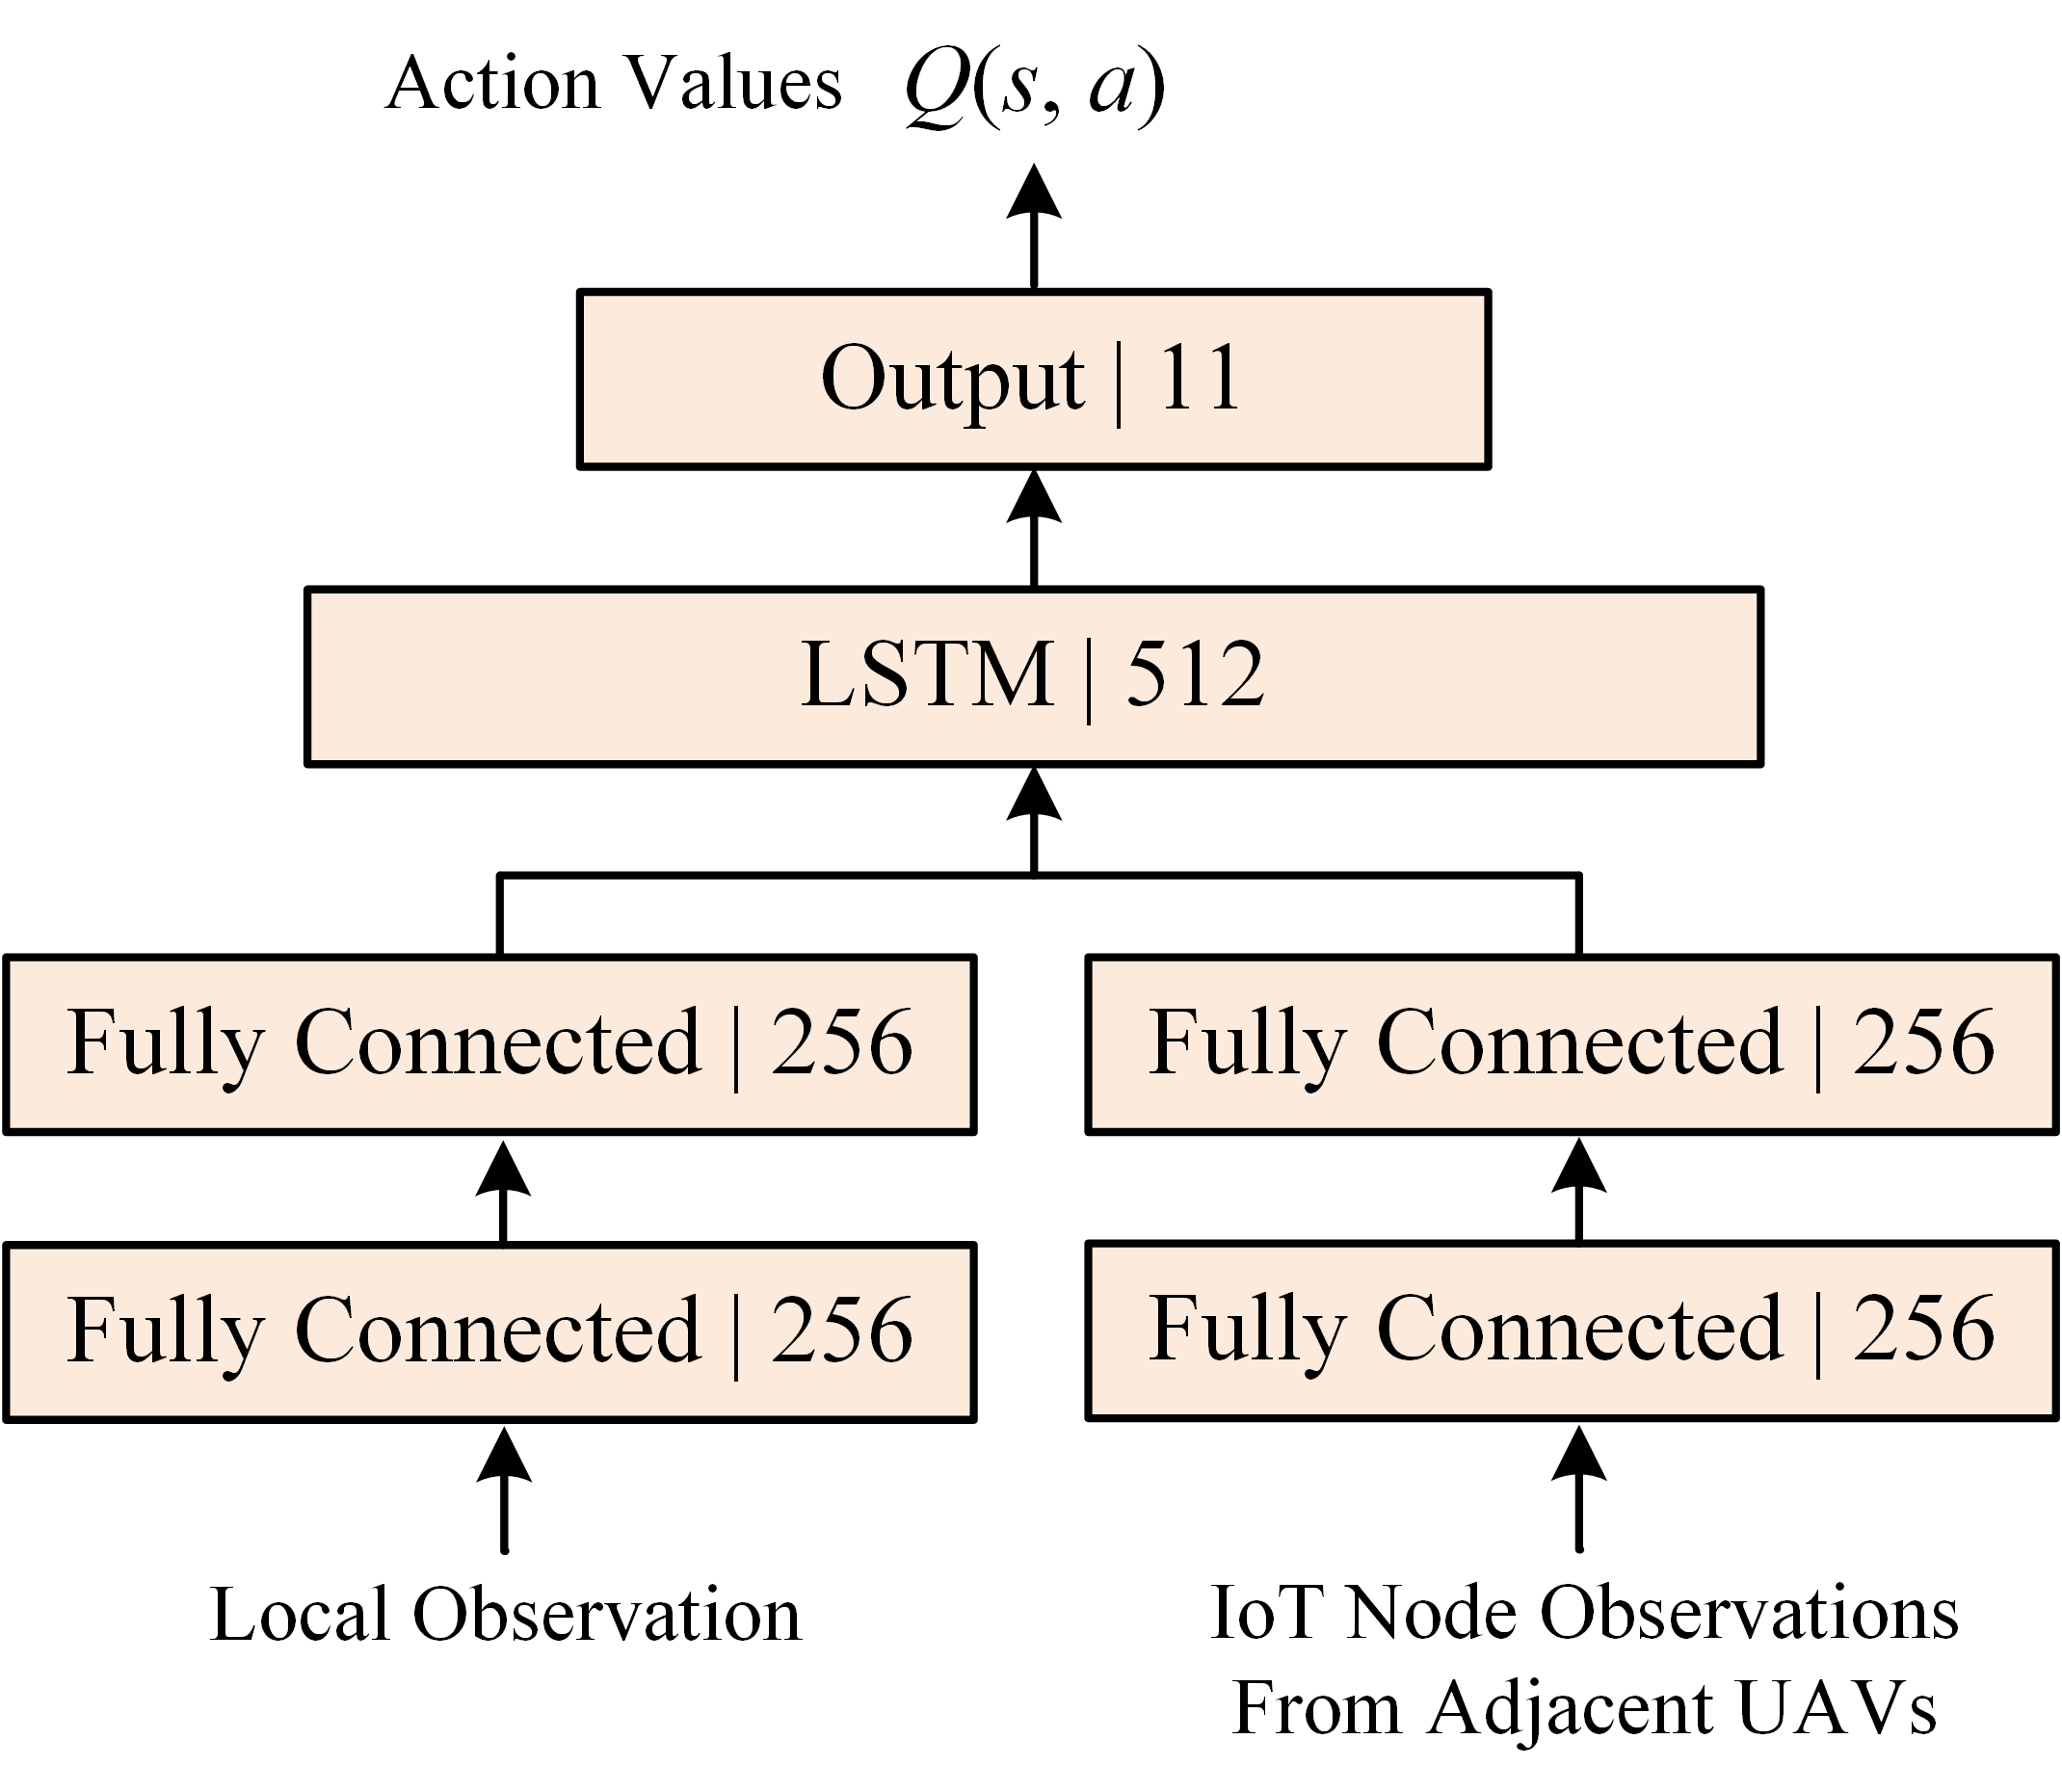
\includegraphics[width=0.35\textwidth]{fig/Network_Collaboration.png}
%    \caption{The neural network structure of collaborative DRQN.}\label{network_collaboration}
%\end{figure}
\subsection{Training}\label{training}

The neural networks in DRQN are stochastically initialized and iterate to an optimal policy network by the experience the UAV obtained from exploration in the environment. Each agent has an experience buffer that is designed to store the information for the updating of policy network. In the experience buffer of $U_i$, the stored information is denoted as 
\begin{equation}\label{exp_pool}
D_i=\left\{\mathcal{O}_i, \mathcal{A}_i, \mathcal{R}_i, \mathcal{O}_i'\right\}, 
\end{equation}
where $\mathcal{O}_i$, $\mathcal{A}_i$, $\mathcal{R}_i$, $\mathcal{O}_i'$ are the sets of experienced observation, action, reward and next observation in the same time slot. When the $U_i$ made action decision at each time slot, the obtained experience $\left({o^i_t, a^i_t, r^i_t, o^i_{t+1}}\right)$ is stored at experience pool $D_i$ by order of time. 

The policy network is updated by mini-batch gradient descent. In each iteration of policy network, the loss is calculated using (\ref{loss_func}) by a mini-batch of experiences randomly sampled from experience pool $D_i$. The gradient of loss updates all the parameters of policy network by backward propagation. The iteration of policy network is independent from the decision making sequence of UAV because of the random sampling, making the network model converges quickly and adapt to the randomly initialized environment model. 

The training process contains two parts. One is the UAV explore at the environment to collect experiences and the other is the policy model updates every $N_P$ decision processes. Algorithm \ref{alg1} gives the pseudo-code of the proposed algorithm in each agent. 

\begin{algorithm}[h]	
	Initialize the policy network parameters $\theta$ and the target network parameters $\theta '$ with $\theta '\gets \theta$\;
	Initialize Experience Pool $D$\;
	\For{$episode=1,2,\cdots,E$}
	{
		Initialize the environment\;
        Clear the memory of LSTM\;
		Receive first local observation $o^l_{t}$\;
		\While{$terminal \neq True$}
		{
            Exchange observation with adjacent UAVs and obtain $o^a_t$\;
            $o_t=\left(o^l_{t}, o^a_t\right)$\;
			Choose an action $a_{t}$ based on $o_t$\;
            Apply action $a_{t}$ to the environment, obtain next local observation $o^l_{t+1}$, reward $r_{t}$, end state flag $terminal$\;
            Push transition $(o_t, a_t, r_t, o_{t+1})$ into $D$\;
            \If{Length of $D$ exceeds training threshold}
            {
                Randomly Sample a mini-batch of transitions $(o_i, a_i, r_i, o'_{i})$ from $D$\;
                Update policy network $\theta$ using (\ref{loss_func}) every $N_P$ decision processes\;
                Update target network $\theta '$ by (\ref{update_target}) every 100 iterations of policy network\;
            }
            Clear the memory of LSTM every $L$ steps\;
            $o^l_{t} \gets o^l_{t+1}$\;
		}
	}
	\caption{Proposed algorithm}\label{alg1}
\end{algorithm}

\section{Experimental results}\label{Experiments}
In this section, the settings of experiment is illustrated. Performance comparisons among proposed method and benchmarks are described from the perspectives of data collection efficiency, handing moving obstacles and multi-UAV collaboration. 

\subsection{Experiment setup}\label{exp_settings}
Experiments in this work are simulated by Python. Both IoT sensor nodes and obstacles are randomly distributed following an uniform distribution throughout an area covers 1km\textsuperscript{2}. Obstacles are set as cylinders whose radii are randomly assigned. The stored data in each IoT sensor node are randomly generated within 5MB. 3 UAVs are dispatched, and the flying height and velocity of each UAV are set as 50m and 10m/s. The energy storage of each UAV is sufficient for 400s of flight. All the UAVs make and execute trajectory planning decisions simultaneously at intervals $\Delta T$ of 1s. 
The parameters for the simulation are set as table \ref{parameters} shows. 
\begin{table*}[tb]
	\renewcommand{\arraystretch}{1.3}
	\caption{The parameter settings for simulation.\label{parameters}}
	\centering
	\begin{tabular}{c|c|c|c|c|c}
		\hline \hline
        \multicolumn{6}{c}{Parameters of communication model} \\ \hline
		\textbf{Parameter} & \textbf{Value} & \textbf{Parameter} & \textbf{Value} & \textbf{Parameter} & \textbf{Value} \\ \hline
		Carrier frequency $f_c$ & 2.4GHz & Noise power $\sigma ^2$ & -90dBm & Communication range $d^{I}_{\max}$  & 50m\\ \hline
        Bandwidth $B$ & 1MHz & Signal transmission power $P$ & -20dBm & Decaying factors $\mu_{LoS}$, $\mu_{NLoS}$ & 3, 4 \\ \hline
		Channel parameters $\alpha$, $\beta$ & 10, 0.6 & & & & \\ \hline 
        %Reward constants $K_1$, $K_2$, $K_3$ & -5, -5, -0.05 & Obstacle buffer distances $d_{\min}^{B}$, $d^{B}_{c}$ & 10m, 20m & UAV separation distances $d^{U}_{\min}$, $d^{U}_{c}$ & 10m, 20m \\
        %Reward factors $\alpha_{1}$, $\alpha_{2}$ & 0.15, 1 & Reward factors $\omega_{D}$, $\omega_{R}$ & 0.5, 0.1 & Scaling factors of fairness $\beta_I$, $\beta_U$ & 1, 1 \\ %\hline
        \multicolumn{6}{c}{Parameters of the proposed algorithm} \\ \hline
        \textbf{Parameter} & \textbf{Value} & \textbf{Parameter} & \textbf{Value} & \textbf{Parameter} & \textbf{Value} \\ \hline
        Learning rate of policy network & 0.0001 & Batch size $N_B$ & 16 & Size of experience buffer $L_B$  & 80,000 \\ \hline
        Discount factor $\gamma$ & 0.95 & Iteration period $N_P$ & 10 & & \\ \hline \hline
	\end{tabular}
\end{table*}
%\begin{table}[h]
%%	\setlength{\abovecaptionskip}{-0.02cm}
%	\renewcommand{\arraystretch}{1.3}
%	\caption{Hyperparameter settings for deep reinforcement learning.\label{hyperparameters}}
%	\centering
%	\begin{tabular}{c|c}%{C{0.1\textwidth}||L{0.33\textwidth}}
%		\hline \hline
%		Hyperparameters & Values  \\ \hline
%		Learning rate & 0.0001 \\ \hline
%		Discount factor $\gamma$ & 0.95 \\ \hline  
%		Batch size $N$ & 16  \\ \hline
%		Size of experience pool  & 80,000 \\ \hline
%        Memory length of LSTM layer $L$  & 10 \\ \hline
%        Iteration period of target network $N_T$  & 100 \\ \hline
%		\hline  		
%	\end{tabular}
%\end{table}
\begin{figure*}[htbp]
	\centering
    %	\setlength{\abovecaptionskip}{-0.03cm}
    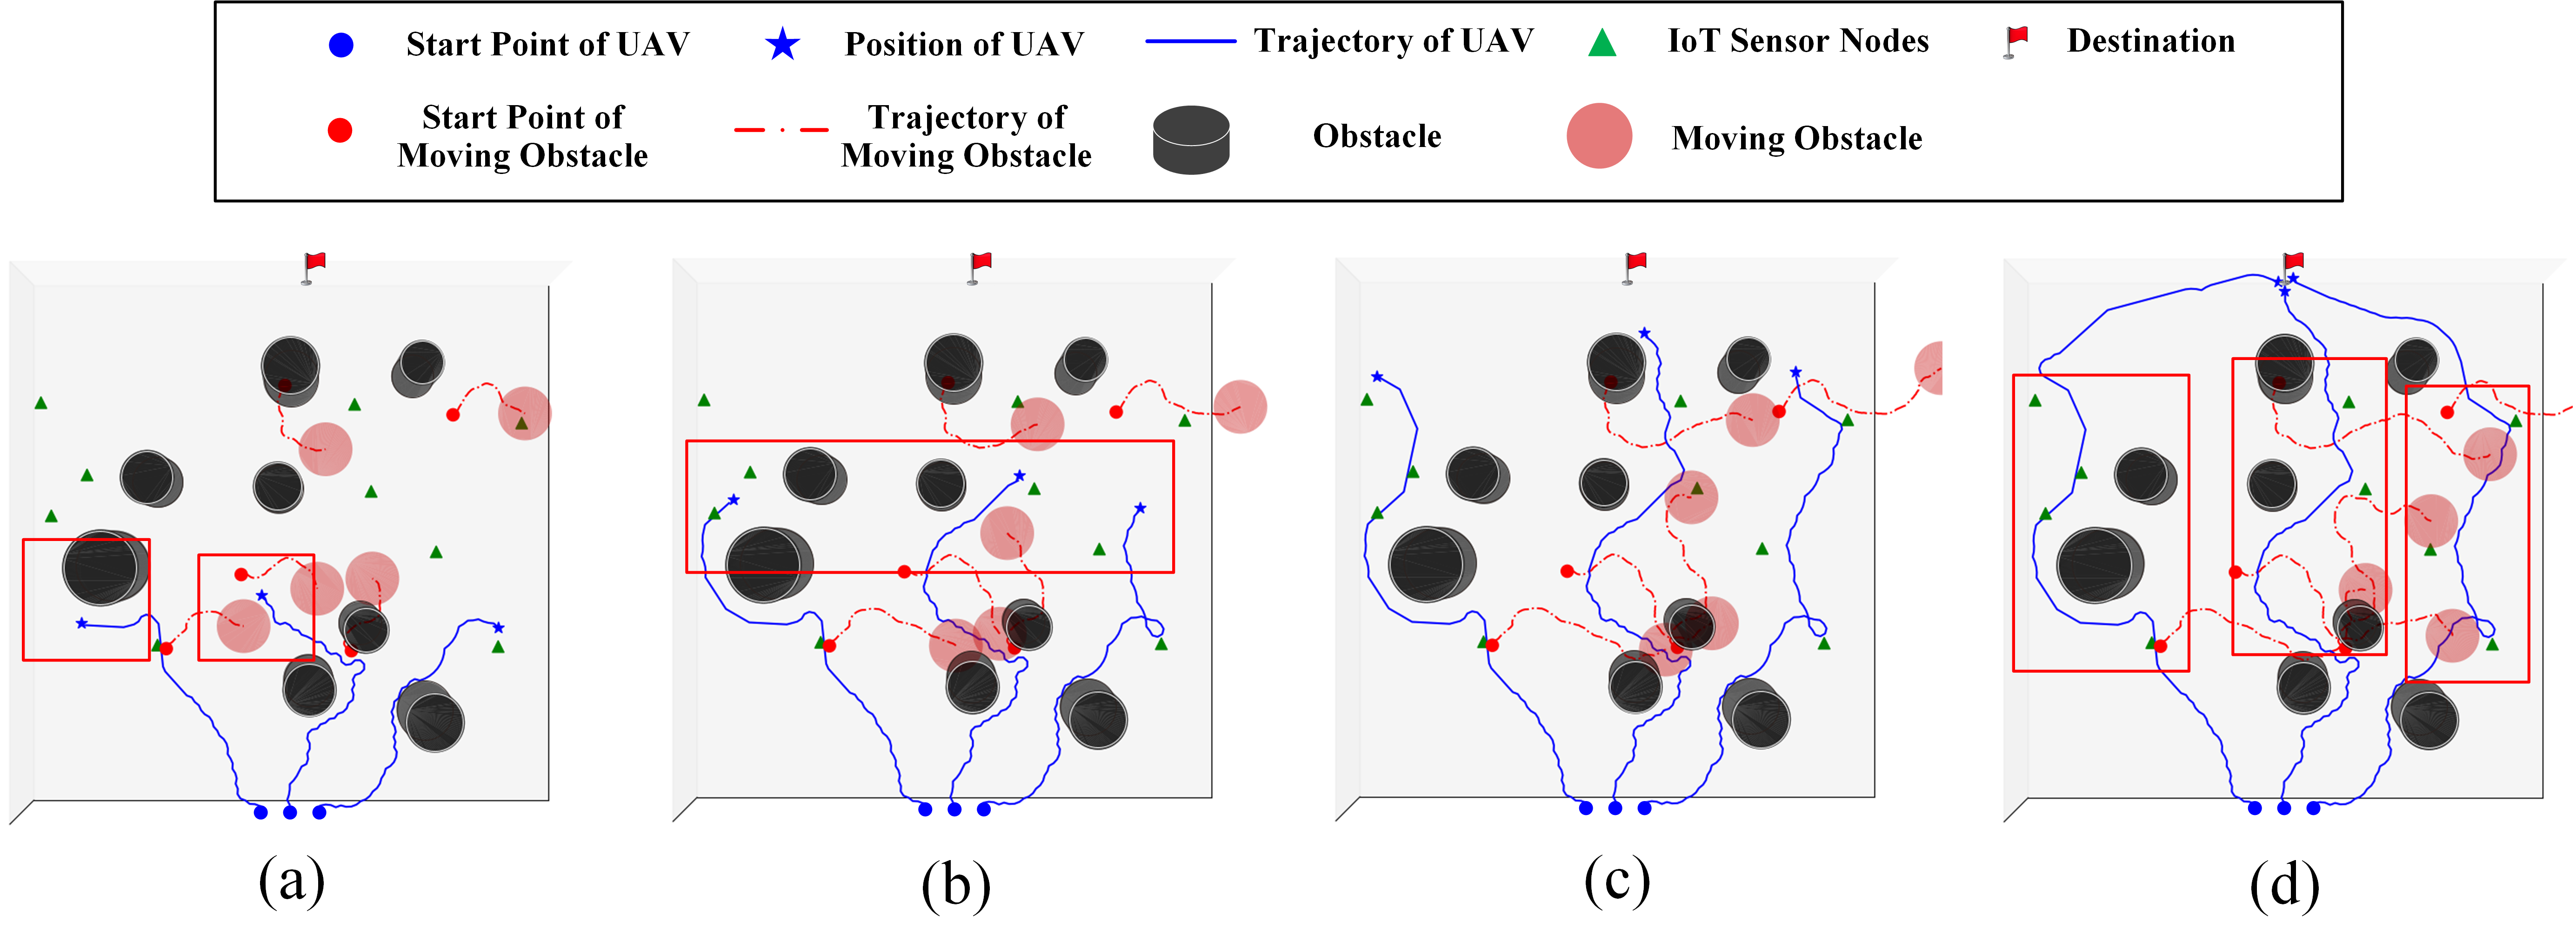
\includegraphics[width=16.5cm]{fig/Traj.png}
    \caption{The UAV trajectories in a data collection episode: (a) at 60s; (b) at 99s; (c) at 130s; (d) at 172s (finished). }\label{trajectory_fig}
\end{figure*}

%In the training of proposed algorithm, the components of the environment are randomly set. The number of IoT nodes is selected from 10 to 26. The number of static obstacles is selected from 3 to 11. The number of moving obstacles is selected from 3 to 8. 

As a comparison, three DRL-based multi-UAV path planning algorithms for data collection are deployed in this experiment. The details of benchmarks are as follows: 
\begin{itemize}
    \item[(a)]\textit{Distributed DRQN:} A fully distributed multi-agent DRQN algorithm without collaboration design. Its structure is same as the algorithm but the neural network for processing sensor node observations form adjacent UAVs and the reward for collaboration are removed. 
    \item[(b)]\textit{Centralized MADRL:} The algorithm proposed in \cite{SXu22}. It is a multi-agent DRL algorithm that use a centralized neural network to process the observations from all the agents. 
    \item[(c)]\textit{D3QN:} The algorithm proposed in \cite{XWang22}. It is a non-cooperative distributed dueling double deep Q-network (D3QN)-based algorithm. 
\end{itemize}

The capability of finishing data collection task for well trained policy model is evaluated by experiment of performance test. In performance test the UAVs make trajectory planning in the environment by the well-trained policy. Some numerical metrics are defined and summarized in performance test. The definitions of metrics are the followings: 
\begin{itemize}
    \item\textit{Success rate:} A successful data collection task is determined when all UAVs arrived at their own landing positions. The success rate is the proportion of successful tasks in all the performance testing tasks. 
    \item\textit{Data collecting rate:} Data collecting rate is the ratio of collected data of IoT nodes to all the data required to be collected. This metric is only summarized when the task is successful. 
    \item\textit{Collision rate:} A collision occurs when any one UAV collided with obstacle or other UAV in the task. Collision rate is the ratio of collision tasks to all the performance testing tasks. 
    \item\textit{Average time:} This metric is defined as the average time a single UAV costs to finish the data collection task. 
\end{itemize}
\subsection{UAV trajectories}\label{trajectory}
Fig. \ref{trajectory_fig} shows the UAV trajectories planned by proposed algorithm in a data collection scenario that contains 9 IoT sensor nodes, 8 static obstacles and 5 moving obstacles. At 60s, UAVs navigate around obstacles that obstruct their ways to IoT sensor nodes. The middle UAV makes response to the oncoming moving obstacle. From 99s to 130s, UAVs traverse IoT sensor nodes and collect the stored data. UAVs select IoT sensor nodes without conflict. The node collection sequences are appropriate for minimum completion time. At 172s, all the UAV finish data collection and arrive at the destination. During inter-node travels, UAVs exhibit smooth trajectories. The quantities of served IoT sensor nodes across all UAVs in a swarm are same. The trajectories demonstrate that UAVs can find appropriate routes for data collection and cooperate well with adjacent UAVs for even workload allocation. 

%\begin{figure*}[htbp]
%	\centering
%	\subfigure[\quad Initial state]{
%		\centering
%		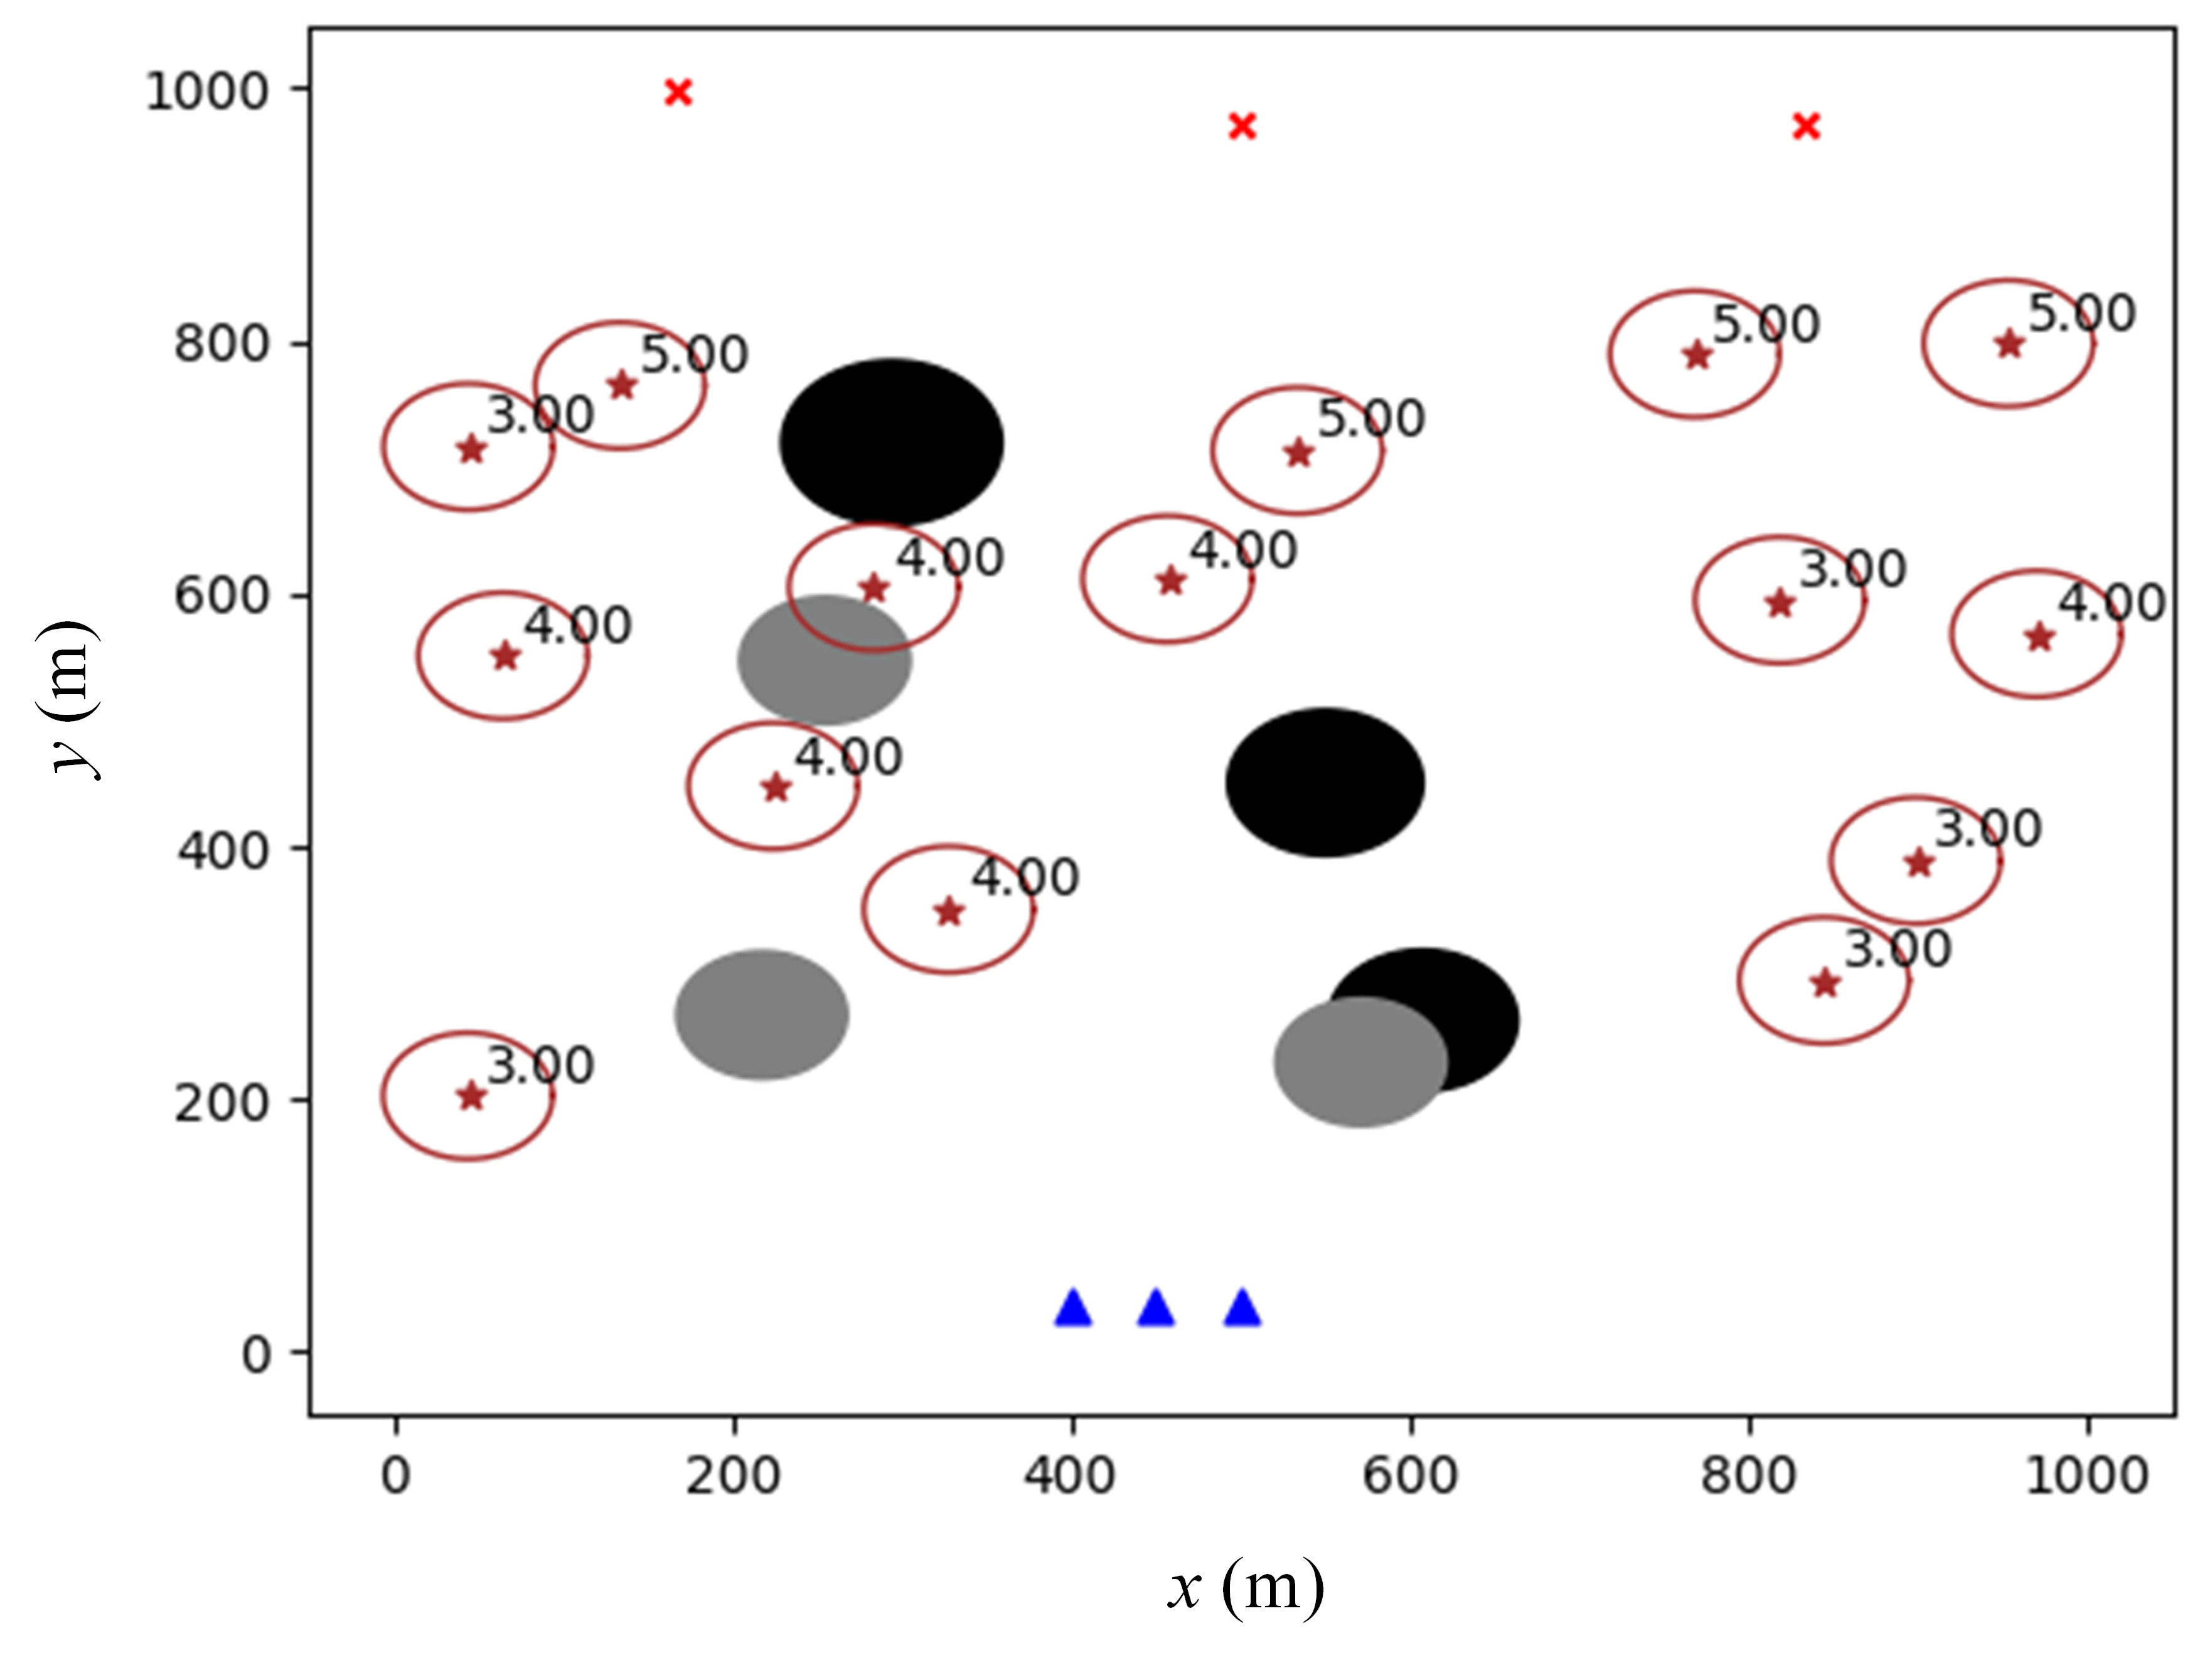
\includegraphics[width=4.2cm]{fig/Trajectory/Initial.png}
%		\label{fig_traj_init}
%	}
%	\subfigure[\quad DRQN-based algorithm]{
%		\centering 
%		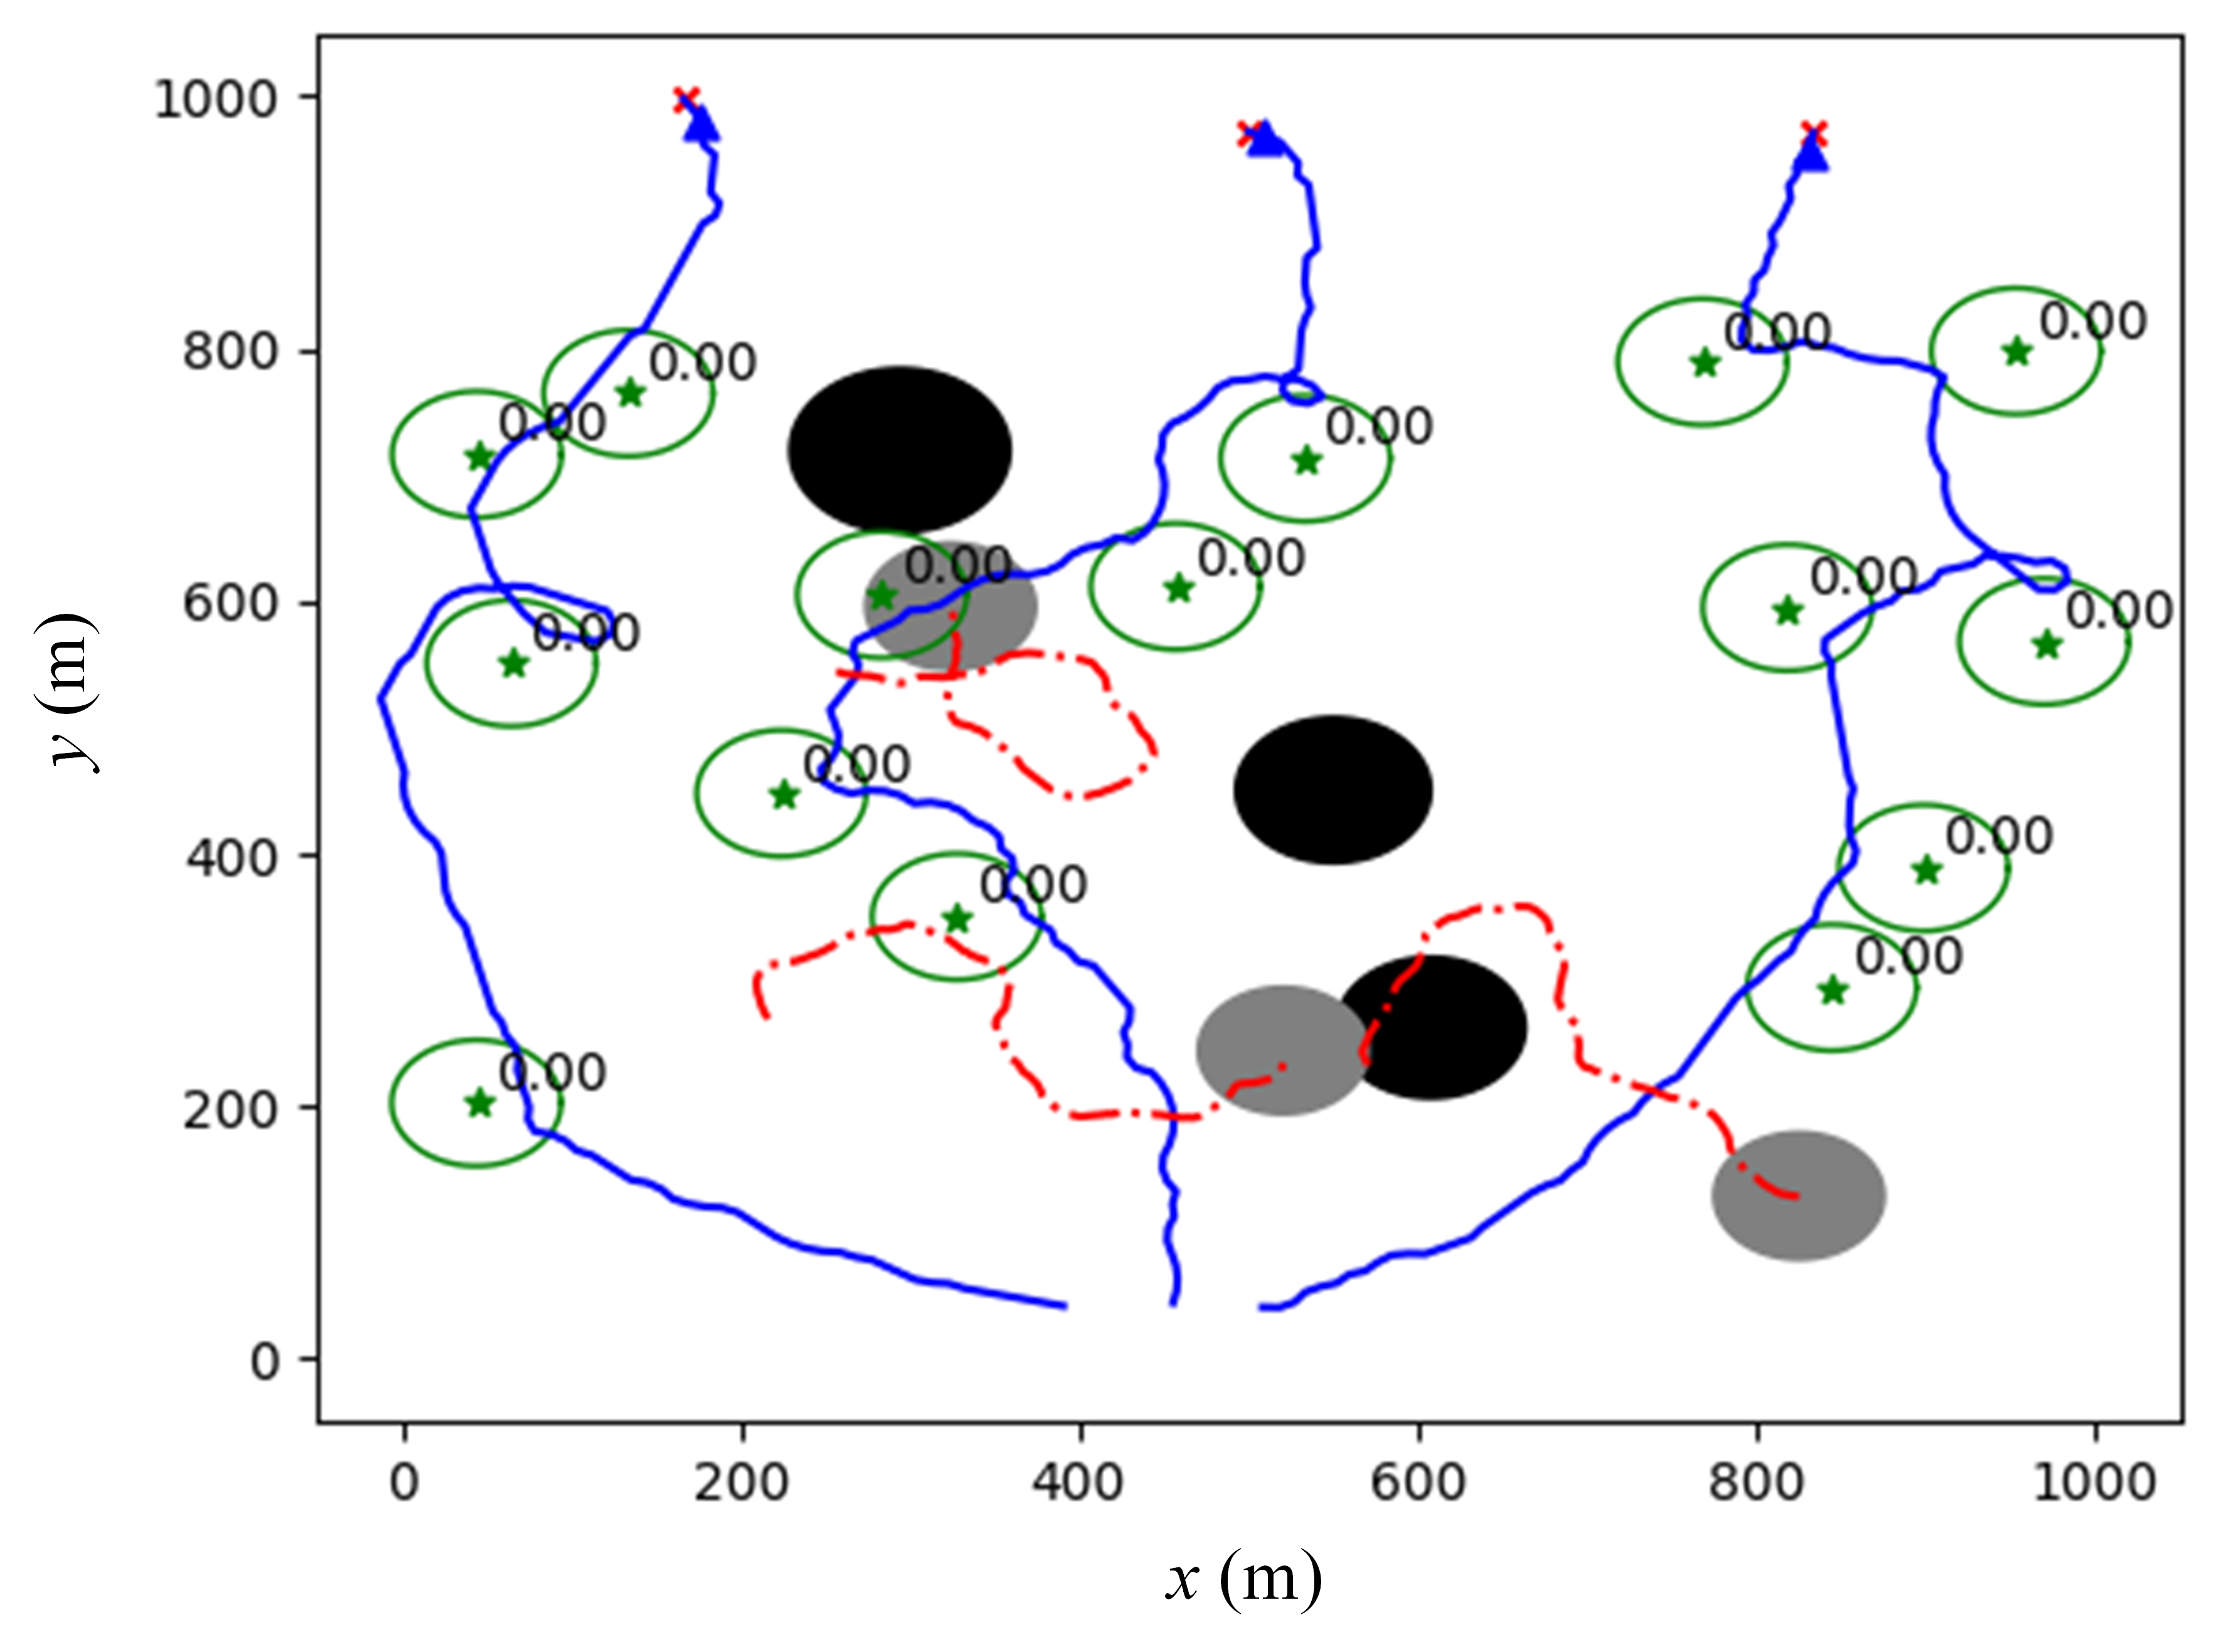
\includegraphics[width=4.2cm]{fig/Trajectory/DRQN.png}
%		\label{fig_traj_drqn}
%	}
%	\subfigure[\quad DQN-based algorithm]{		
%		\centering 
%		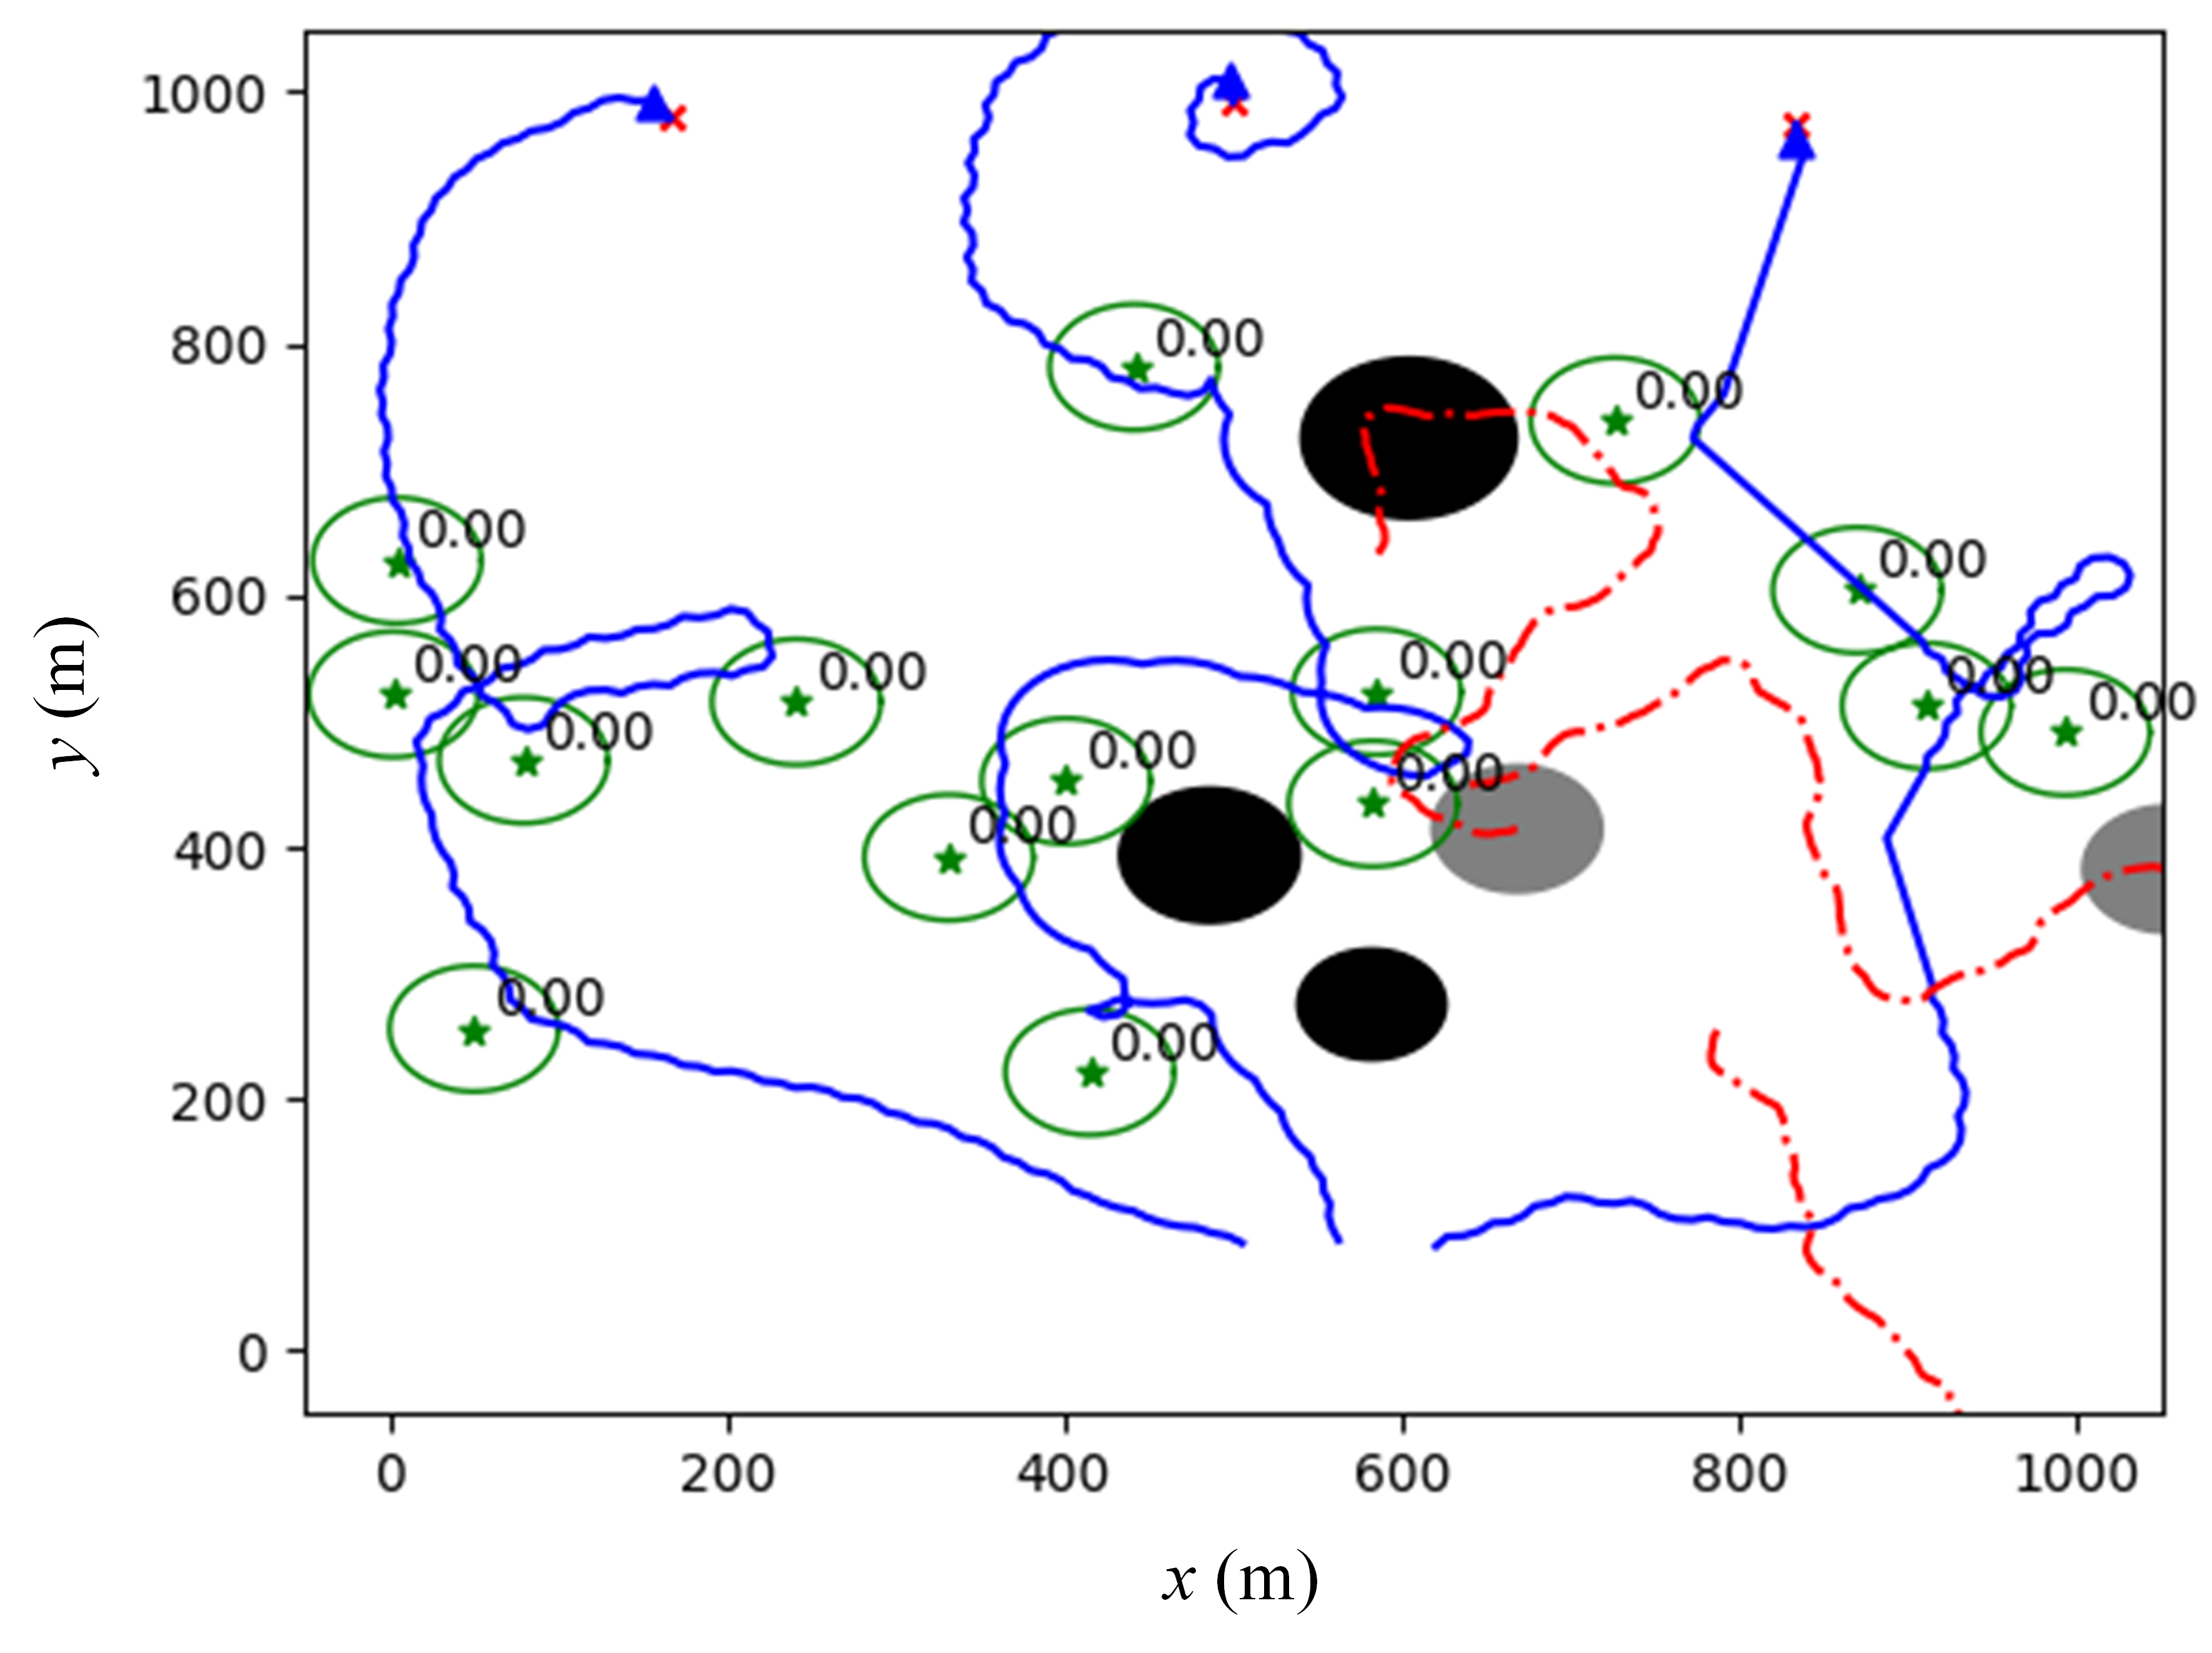
\includegraphics[width=4.2cm]{fig/Trajectory/DQN.png}
%		\label{fig_traj_dqn}
%	}
%	\subfigure[\quad D3QN-based algorithm]{		
%		\raggedright
%		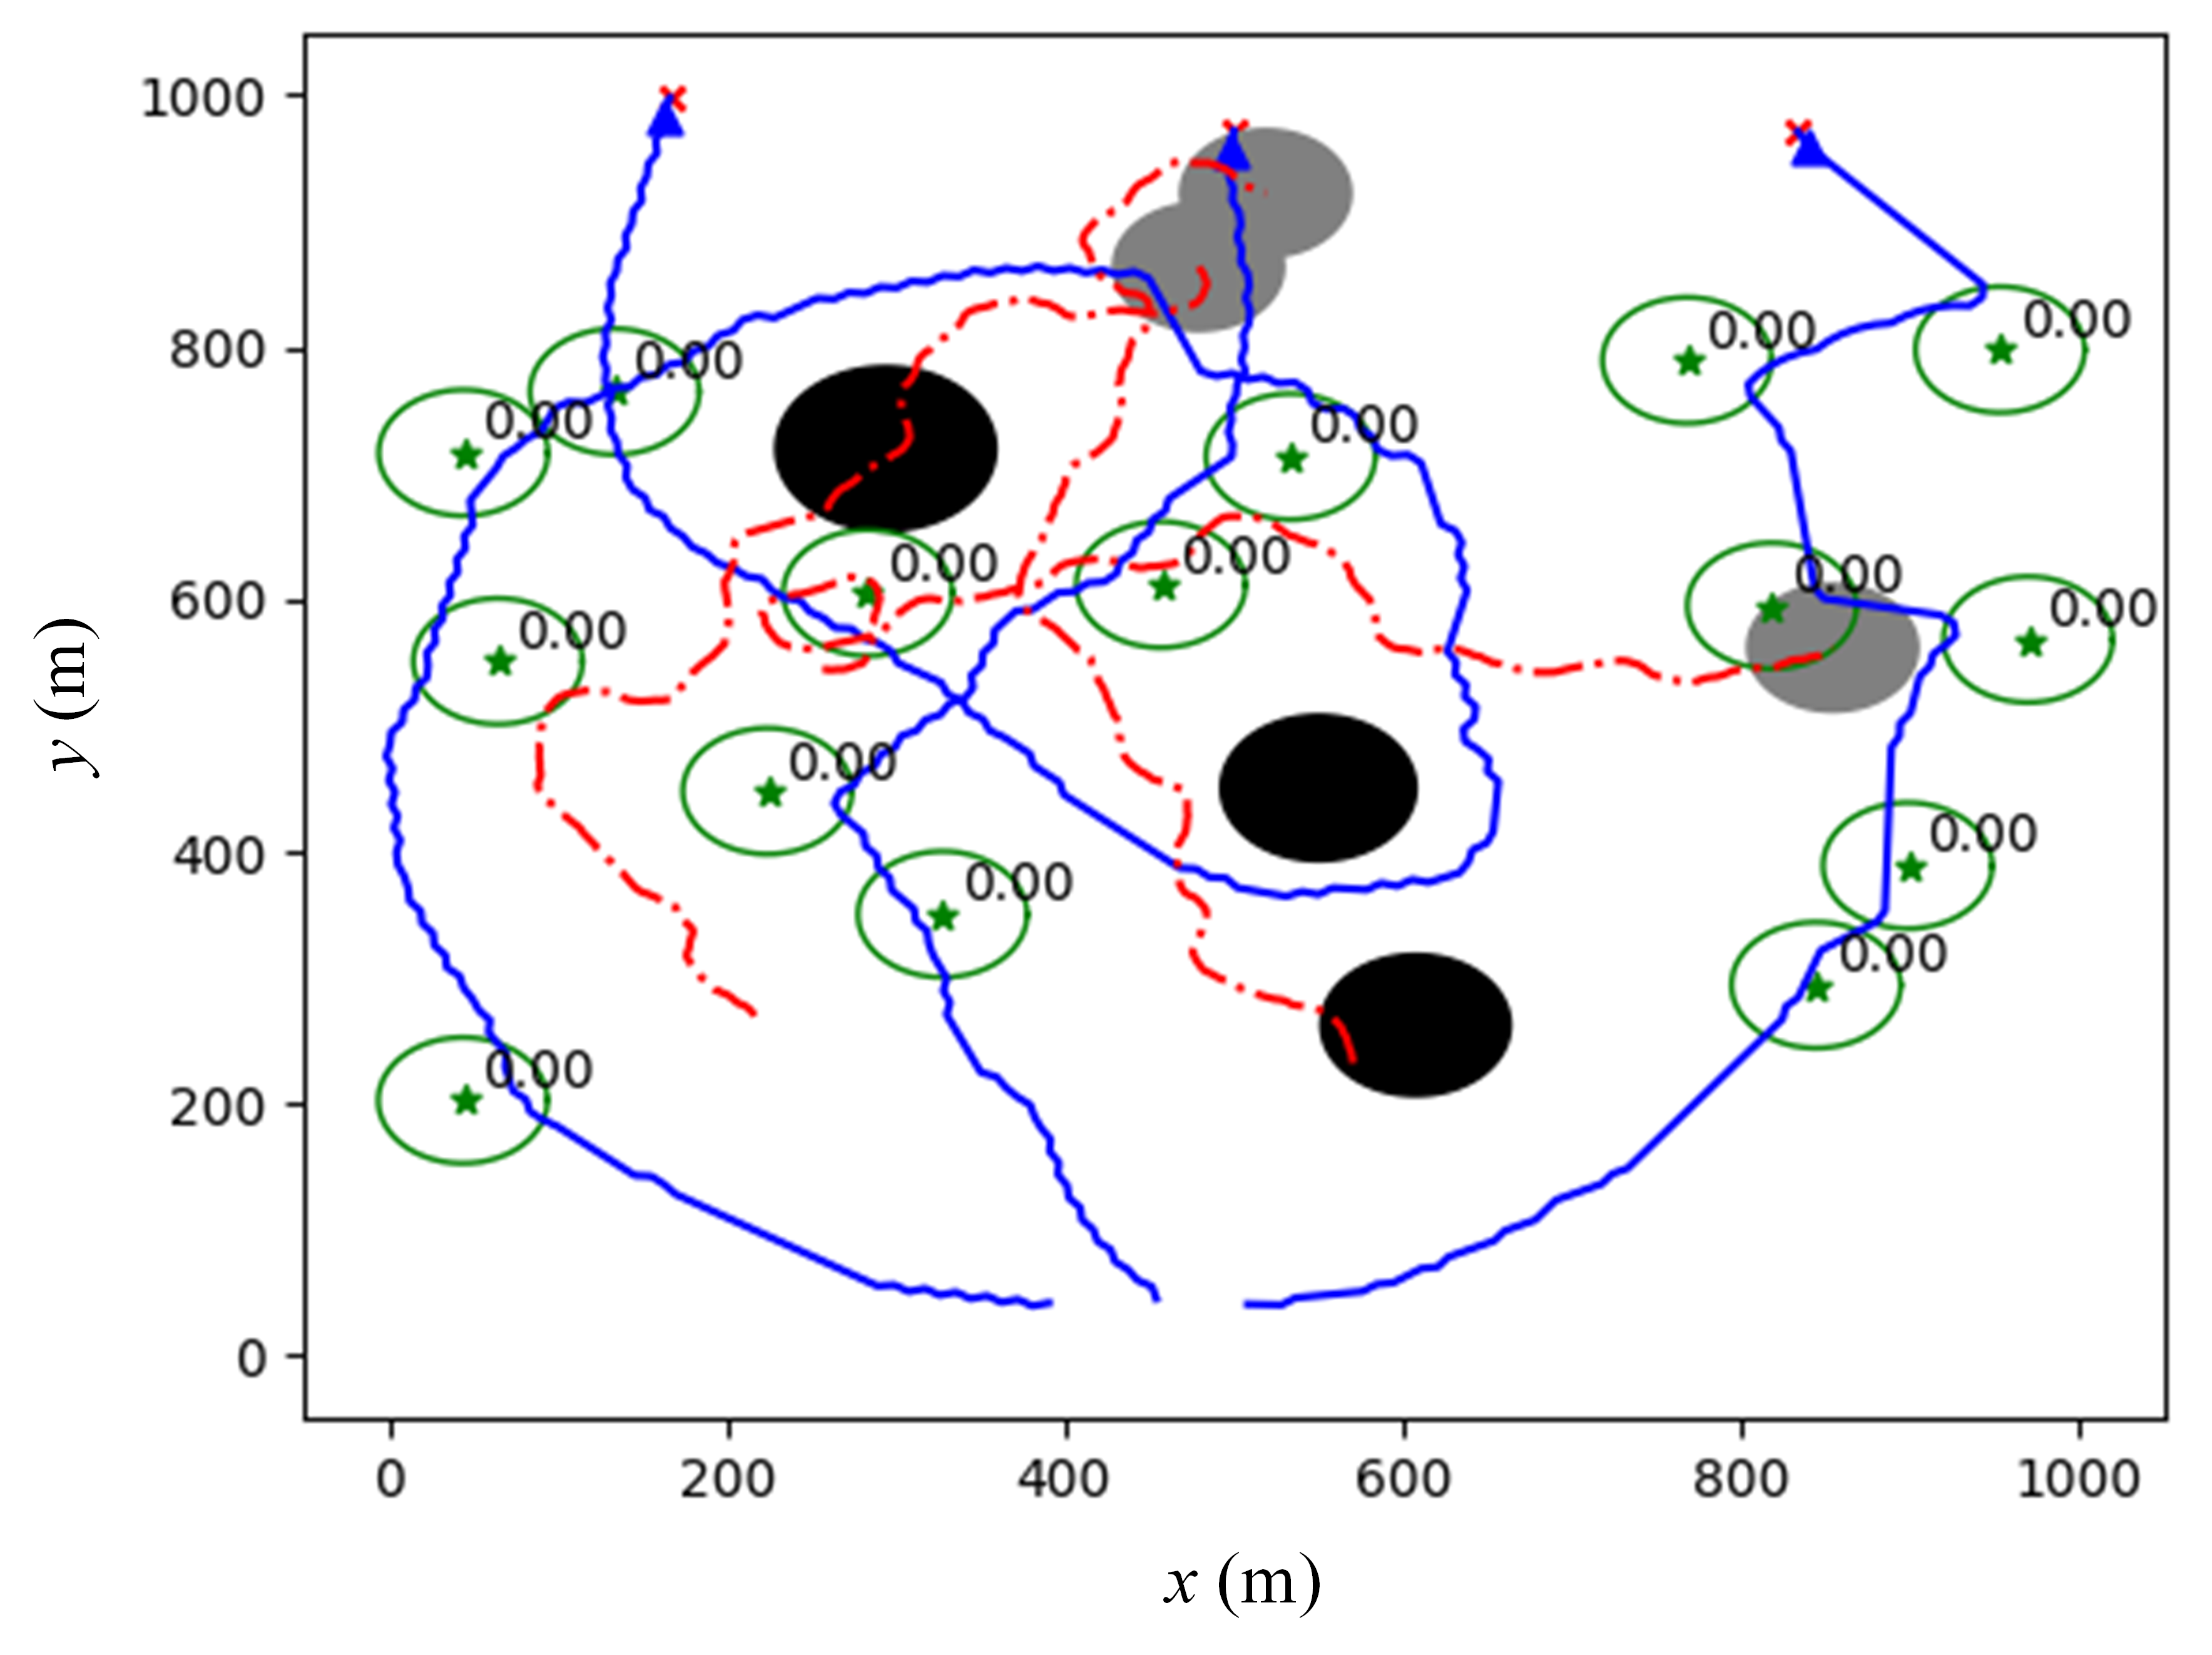
\includegraphics[width=4.2cm]{fig/Trajectory/D3QN.png}	
%		\label{fig_traj_d3qn}
%	}		
%	\caption{The trajectories of UAVs using different algorithms in data collection task: (a) Initial state; (b) DRQN-based algorithm; (c) DQN-based algorithm; (d) D3QN-based algorithm. Note that the green circle is the communication range of IoT sensor node, the blue solid line is the trajectory of UAV and the dash-dot-line is the trajectory of moving obstacles. Environment contains 3 static obstacles, 3 moving obstacles and 15 IoT sensor nodes \label{trajectory}} 					
%\end{figure*}
%\subsection{Network Model Convergence}
%
%We train the path planning model for 2000 episodes using DRQN, D3QN and DQN. The received reward of agent in single episode is summarized during training process to reflect the training performance of algorithm. Model iteration starts when the stored experience exceed 3000 tuples. As is demonstrated in Fig. \ref{convergence_perf}, the all the reward curves ascended after about 75 training episodes. It can be attributed to the models based on all these algorithms start accumulate adequate experience for iteration at about 75 episodes and learn the path planning policy at a similar rate. After 350 training episodes, all the reward curves converged at the same level. It shows that all the policy model learned their own optimal policy and their policies are similar form the perspective of episode reward. To further verification the performance of these algorithms, their trained policies will be tested in data collection application. 
%\begin{figure}[htbp]
%	\centering
%	%	\setlength{\abovecaptionskip}{-0.03cm}
%	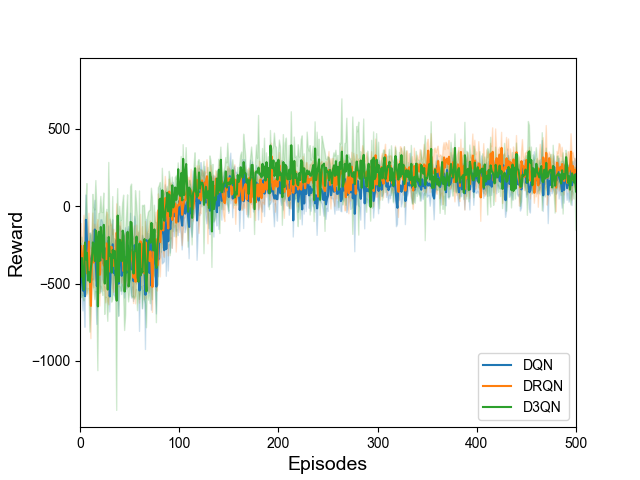
\includegraphics[width=0.45\textwidth]{fig/Reward.png}
%	\caption{Convergence performance of DRQN, D3QN and DQN \label{convergence_perf}}
%\end{figure} 
\begin{figure*}[htbp]
	\centering
	\subfigure[\quad Success rate]{
		\centering
		
\includegraphics[width=4.2cm]{fig/IoT_node_test/Successrate.png}
		\label{fig_perf_iot_sr}
	}
	\subfigure[\quad Data collection rate]{
		\centering 
		
\includegraphics[width=4.2cm]{fig/IoT_node_test/Data_collection_rate.png}
		\label{fig_perf_iot_dcr}
	}
	\subfigure[\quad Collision rate]{		
		\centering 
		
\includegraphics[width=4.2cm]{fig/IoT_node_test/Collision_rate.png}
		\label{fig_perf_iot_cr}
	}
	\subfigure[\quad Average time]{		
		\raggedright
		
\includegraphics[width=4.2cm]{fig/IoT_node_test/Avgtime.png}	
		\label{fig_perf_iot_at}
	}		
	\caption{Data collection path planning performance in different number of IoT sensor nodes: (a) success rate; (b) data collection rate; (c) collision rate; (d) average time. Note that the average time is in seconds. \label{perf_iot_nodes}} 				
\end{figure*}
\begin{figure*}[htbp]
	\centering
	\subfigure[\quad Success rate]{
		\centering
		
\includegraphics[width=4.2cm]{fig/Obstacle_test/Successrate.png}
		\label{fig_perf_obs_sr}
	}
	\subfigure[\quad Data collection rate]{
		\centering 
		
\includegraphics[width=4.2cm]{fig/Obstacle_test/Data_collection_rate.png}
		\label{fig_perf_obs_dcr}
	}
	\subfigure[\quad Collision rate]{		
		\centering 
		
\includegraphics[width=4.2cm]{fig/Obstacle_test/Collision_rate.png}
		\label{fig_perf_obs_cr}
	}
	\subfigure[\quad Average time]{		
		\raggedright
		
\includegraphics[width=4.2cm]{fig/Obstacle_test/Avgtime.png}	
		\label{fig_perf_obs_at}
	}		
	\caption{Data collection path planning performance in different number of moving obstacles: (a) success rate; (b) data collection rate; (c) collision rate; (d) average time. Note that the average time is in seconds. \label{perf_obstacles}} 				
\end{figure*}
\subsection{Performance of data collection}
Fig. \ref{perf_iot_nodes} shows the data collection performance when the number of IoT sensor nodes is varying. The environment has 5 static obstacle, 5 moving obstacle and varying number of IoT sensor nodes. 3 UAVs are dispatched to perform data collection. As shown in Fig. \ref{fig_perf_iot_sr}, when the environment contains 15 IoT sensor nodes, the collaborative DRQN exhibits improvement on success rate by 3.5\% compared to centralized MADRL, by 7.5\% compared to distributed DRQN and by 16.5\% compared to D3QN. The collaborative DRQN method and centralized MADRL method exhibits higher success rate compared to the distributed DRQN and D3QN. This is because path planning of each UAV is allocated well to avoid the competition of sensor node selection between UAVs in collaborative DRQN and centralized MADRL. The success rate of D3QN method is much lower than others is because the data collection reward in this algorithm is only related to the amount of collected data, making the UAV agent cannot find an effective collection sequence. As the collected data is counted only when data collection task is success, D3QN method demonstrates data collection rate but low success rate implicates that it makes UAVs concentrate on inefficient IoT sensor node searching, making the time cost exceeds limitation. As shown in Fig. \ref{fig_perf_iot_dcr}, all the methods attain success rates greater than 99\%. This is because UAVs can discover most of IoT sensor nodes and collect the data before arrive at destination. As shown in Fig. \ref{fig_perf_iot_cr}, the centralized MADRL method exhibits lower collision rate compared to collaborative DRQN method. This is because the centralized MADRL method better coordinates all the UAVs to avoid the obstacles. The lower collision rate of distributed DRQN method compared to those of collaborative DRQN method and centralized MADRL is attributed to that distributed DRQN method has higher probability of occurring conflict between adjacent UAVs. As shown in Fig. \ref{fig_perf_iot_at}, when the number of IoT sensor nodes in each data collection task is 18, the average time cost of collaborative DRQN method is reduced by 4.03\% compared to centralized MADRL, 6.87\% compared to distributed DRQN and 9.04\% than D3QN. This is because collaborative DRQN method makes each UAV coordinate data collection workload with adjacent UAVs to utilize the data collection capability of the whole multi-UAV system. These results show that compared to distributed DRQN and D3QN, collaborative DRQN can handle the increasing number of IoT sensor nodes by the cooperation of UAVs, and compared to centralized MADRL, the UAVs using collaborative DRQN are more likely to find shorter trajectories by their independent path planning models. 

\subsection{Performance of handling complex environment}
The complexity of environment is represented by the number of static and moving obstacles that are randomly distributed in the environment. Fig. \ref{perf_obstacles} shows the data collection performance when the number of moving obstacles is varying. The environment has 15 IoT sensor nodes, 5 static obstacle and varying number of moving obstacles. 3 UAVs are dispatched to perform data collection. As shown in Fig. \ref{fig_perf_obs_sr}, when the environment contains 6 moving obstacles, the collaborative DRQN exhibits improvement on success rate by 1.8\% compared to centralized MADRL, by 3.9\% compared to distributed DRQN and by 15.2\% compared to D3QN. The D3QN method demonstrates a much lower success rate, because this method is hard to make accurate reaction to unexpected obstacles. As shown in Fig. \ref{fig_perf_obs_cr}, the collision rates of collaborative DRQN method, centralized MADRL method and distributed DRQN are also similar. Compared to the centralized MADRL method, the collaborative DRQN method is less advantageous on avoiding collisions, because centralized MADRL processes obstacle observations from all the UAVs, which makes the UAV group easier to discover obstacles. The performance of D3QN method on higher collision rate compared to others shows that collision is the main factor causing the failure of data collection task. As shown in Fig. \ref{fig_perf_obs_dcr}, the data collection rates of collaborative DRQN method, centralized MADRL method and distributed DRQN are close to 100\%. As shown in Fig. \ref{fig_perf_obs_at}, when the environment contains 6 moving obstacles, the collaborative DRQN method exhibits a reduction on average completion time by 7.47\% compared to the centralized MADRL method, 9.82\% compared to the distributed DRQN method and 10.19\% compared to the D3QN method. The rapid ascent of average completion time of centralized MADRL method is because the agents using centralized policy are excessively sensitive to obstacles and spend more time on avoiding them. These results show that collaborative DRQN method is less affected by complex and dynamically changing environment compared to benchmarks. 
\begin{figure*}[htbp]
	\centering
	\subfigure[\quad Success rate]{
		\centering
		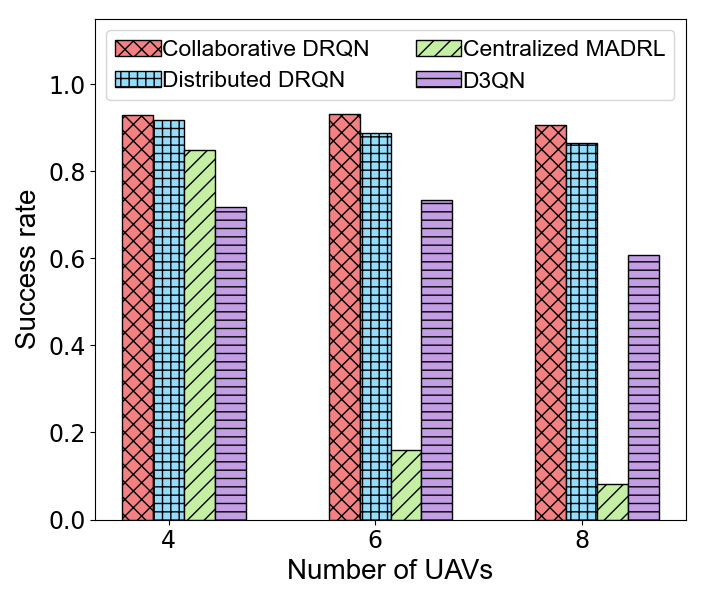
\includegraphics[width=4.2cm]{fig/Collaboration_test/Successrate.png}
		\label{fig_perf_col_sr}
	}
	\subfigure[\quad Data collection rate]{
		\centering 
		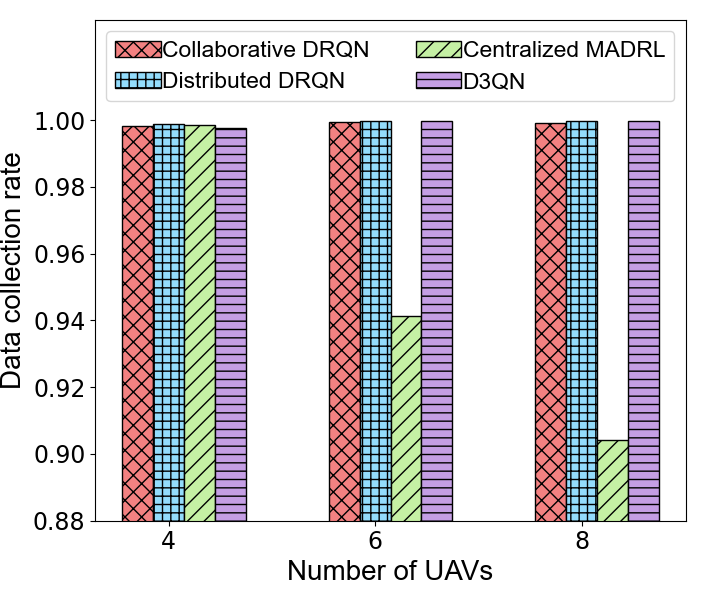
\includegraphics[width=4.2cm]{fig/Collaboration_test/Data_collection_rate.png}
		\label{fig_perf_col_dcr}
	}
	\subfigure[\quad Collision rate]{		
		\centering 
		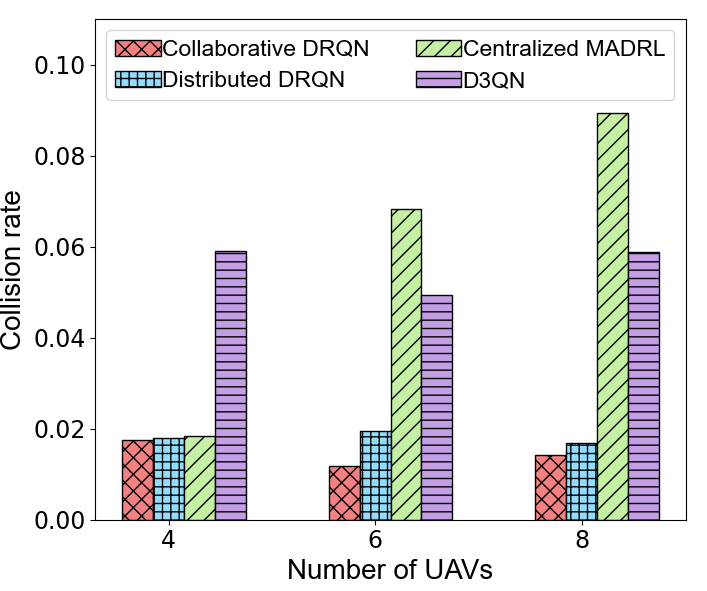
\includegraphics[width=4.2cm]{fig/Collaboration_test/Collision_rate.png}
		\label{fig_perf_col_cr}
	}
	\subfigure[\quad Average time]{		
		\raggedright
		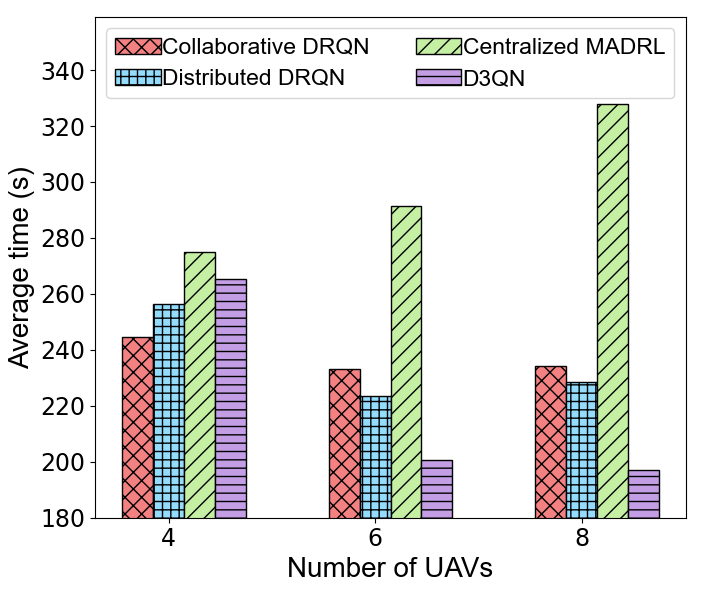
\includegraphics[width=4.2cm]{fig/Collaboration_test/Avgtime.png}	
		\label{fig_perf_col_at}
	}		
	\caption{Data collection path planning performance in different number of IoT sensor nodes: (a) success rate; (b) data collection rate; (c) collision rate; (d) average time. Note that the average time is in seconds. \label{perf_collaboration}} 				
\end{figure*}
%\begin{table*}[tb]
%	\renewcommand{\arraystretch}{1.3}
%	\caption{The collaboration fairness performance.\label{fairness}}
%	\centering
%	\begin{tabular}{c|c|c|c|c}
%		\hline %\hline
%		\quad Algorithm & Collaborative DRQN & Distributed DRQN & Centralized MADRL & \qquad D3QN \qquad\  \\ \hline
%		\quad Success rate & \textbf{95.8}\% & 92.5\% & 93.1\% & \qquad 81.7\% \qquad\  \\ %\hline
%        \quad Average time (s) & \textbf{253.10} & 264.53 & 262.62 & \qquad 287.64 \qquad\  \\ %\hline
%		\quad Fairness on work amount & \textbf{0.875} & 0.847 & 0.860 & \qquad 0.759 \qquad\  \\ %\hline 
%        \quad Fairness on collection time & \textbf{0.907} & 0.899 & 0.888 & \qquad 0.765 \qquad\  \\ \hline
%	\end{tabular}
%\end{table*}
\subsection{Performance of multi-UAV collaboration}
%Table \ref{fairness} describes the collaboration fairness performance in the scenario contains 3 dispatched UAVs, 15 IoT sensor nodes, 8 static obstacles and 5 moving obstacles. Additional 2 metrics are used for fairness evaluation based on the collection result.
%\begin{itemize}
%  \item Fairness on work amount, which is defined by the Jain's fairness based on served IoT sensor nodes among UAVs, indicates the uniformity of UAVs in selecting IoT sensor nodes; 
%  \item Fairness on collection time, which is defined by the Jain's fairness based on the episode time when each UAV finishes data collection of its last scheduled IoT sensor node, indicates the consistency of temporal cost expenditures among UAVs on data collection. 
%\end{itemize} 
%The proposed collaborative DRQN algorithm exhibits the highest fairness on both work amount and collection time implies that UAVs in the swarm are cooperate well to exhibit balanced distribution of collection workloads and time costs among UAVs, resulting in the highest success rate and average completion time. Distributed DQN exhibits high fairness on collection time and short average time This is because the UAVs can plan their routes with optimal completion time in complex environment. The UAV swarm using centralized MADRL coordinates the IoT sensor node selections for data collection well, demonstrating a high fairness on work amount. But the centralized MADRL neglects the time costs for data collection among UAVs, resulting in a relatively diminished fairness on collection time. 

Fig. \ref{perf_collaboration} shows the data collection performance when increasing number of UAVs are dispatched. The environment has 15 IoT sensor nodes, 5 static obstacle and 5 moving obstacles. As shown in Fig. \ref{fig_perf_col_sr}, the experimental group using centralized MADRL method exhibits a sharp decline when more then 5 UAVs are dispatched. This is because input and output of the centralized algorithm dimensionality increase with the number of UAVs. The collaborative DRQN method demonstrates an improvement on success rate achieving 4.3\% and 19.6\% higher performance compared to distributed DRQN and D3QN respectively when 5 UAVs are under the control. As shown in Fig. \ref{fig_perf_col_dcr}, all methods exhibit a data collection rate near 100\% except the centralized MADRL algorithm. As shown in Fig. \ref{fig_perf_col_cr}, the collaborative DRQN and distributed DRQN are stable in collision rate when the number of controlled UAV increases. As shown in Fig. \ref{fig_perf_col_at}, when the swarm has less than 4 UAVs, the collaborative DRQN method exhibits the least average completion time, and when the swarm has more than 5 UAVs, the D3QN and distributed DRQN method exhibit less average completion time compared to collaborative DRQN. In summary, the collaborative DRQN method coordinates a group of UAVs better and demonstrates more stable performance when a large number of UAVs are deployed. 
\begin{table*}[htp]
	%	\setlength{\abovecaptionskip}{-0.02cm}
	\renewcommand{\arraystretch}{1.3}
	\caption{Work load of single UAV.\label{perf_wl_uav}}
	\centering
	\newcommand{\rb}[1]{\raisebox{-1.5ex}[0pt]{#1}}
	\begin{tabular}{C{0.08\textwidth}|C{0.08\textwidth}|C{0.08\textwidth}|C{0.08\textwidth}|C{0.08\textwidth}|C{0.08\textwidth}|C{0.08\textwidth}|C{0.08\textwidth}|C{0.08\textwidth}}
		\hline \hline
		\multirow{2}{0.08\textwidth}{Algorithm} & \multicolumn{2}{c|}{Proposed Algorithm} & \multicolumn{2}{c|}{Distributed DRQN} & \multicolumn{2}{c|}{Centralized MADRL} & \multicolumn{2}{c}{D3QN} \\ \cline{2-9} 
		\multicolumn{1}{c|}{} & Flight Time & Hovering Time & Flight Time & Hovering Time & Flight Time & Hovering Time & Flight Time & Hovering Time \\ \hline

		UAV 1 &  182.27  & 27.53 & 183.76 & 26.63 &  206.56 & 27.57 & 202.16 & 25.38 \\ \hline  

		UAV 2 & 175.30  & 22.73 & 191.62 & 21.6 &  186.99 & 27.41 & 181.97 & 23.96 \\ \hline
		
		UAV 3 & 181.41  & 26.78 & 202.53 & 28.76 &  219.04 & 21.92 & 217.76 & 27.10 \\ \hline
		
		Standard Deviation & 3.1  & 2.11 & 7.7 & 3.0 &  13.19 & 2.62 & 14.65 & 1.28 \\ \hline
		\hline
	\end{tabular}
\end{table*}

%As the environment contains dynamic obstacles with random moving path to simulate complex environment, the performance test in complex environment is conducted by changing the number of dynamic obstacles in the environment. We set the environment contains 3 UAVs, 15 IoT nodes, 5 fixed obstacles. As the number of dynamic obstacles changes from 3 to 7, in each setting of dynamic obstacles, the result after 1000 conducted testing task is shown in Fig. \ref{perf_obstacles}. Fig. \ref{perf_obstacles}(a) illustrates the DRQN-based algorithm has the highest success rate in different numbers of moving obstacles. It illustrates that the DRQN-based algorithm can find the path to finish the data collection and fly to landing position with the best performance. Fig. \ref{perf_obstacles}(b) illustrates the D3QN-based algorithm has the highest data collection rate. It may be attributed to the dueling structure of action value and state value makes UAV focus on the state of closer objects such as the detected surrounding IoT sensor nodes. Fig. \ref{perf_obstacles}(c) illustrates all of the algorithms in this performance test show the similar collision rate, but the D3QN-based algorithms has the lowest result regardless of the number of moving obstacles. It can be attributed to the D3QN-based algorithm has the stronger awareness of the oncoming obstacle. Fig. \ref{perf_obstacles}(d) illustrates DRQN-based algorithm spent the shortest time on finishing data collection task. Compared to DQN-based algorithm, it proved that the RNN can help the DQN find the shortest flying path in the whole environment. 

%%At each single data collection task, the trajectories of UAVs are shown at Fig. \ref{trajectory}. UAVs start at one end of data collection area and land at the other end as illustrated at Fig. \ref{fig_traj_init}. Fig. \ref{fig_traj_drqn} displays the DRQN-based algorithm always makes UAV find a shorter path toward IoT sensor nodes and its landing position. As a comparison, the path of UAV with DQN-based algorithm is longer especially when the UAV approached the landing position as Fig. \ref{fig_traj_dqn} displays. Fig. \ref{fig_traj_d3qn} shows that the UAVs can find the shortest path toward IoT sensor nodes. However, the leftmost UAV was effected by two moving obstacle during its flight, making its path lengthened. It can be attributed to the D3QN-based algorithm always makes UAV keep a longer distance to obstacle. 

%\begin{table*}[tb]
%	\renewcommand{\arraystretch}{1.3}
%	\caption{The performance on data collection of each UAV in a single episode.\label{perf_sing}}
%	\centering
%	\begin{tabular}{c|c|c|c|c}
%		\hline %\hline
%		   & Served IoT nodes & Collected data (MB) & Total flight time (s) & Data collection time (s) \\ \hline
%		 UAV 1 & 5 & 23 & 203 & 182 \\ %\hline
%         UAV 2 & 4 & 17 & 193 & 130 \\ %\hline
%		 UAV 3 & 6 & 25 & 212 & 143 \\ \hline
%         Standard deviation & 0.816 & 3.40 & 7.76 &  22.10 \\ \hline 
%	\end{tabular}
%\end{table*}
%\begin{table*}[tb]
%	\renewcommand{\arraystretch}{1.3}
%	\caption{The average performance on data collection of each UAV.\label{perf}}
%	\centering
%	\begin{tabular}{c|c|c|c|c}
%		\hline %\hline
%		   & Served IoT nodes & Collected data (MB) & Total flight time (s) & Data collection time (s) \\ \hline
%		 UAV 1 & 5 & 19.83 & 200.89 & 142.70 \\ %\hline
%         UAV 2 & 5 & 20.15 & 186.77 & 141.40 \\ %\hline
%		 UAV 3 & 5 & 19.68 & 222.74 & 156.29 \\ \hline
%         Standard deviation & 0 & 0.20 & 14.80 & 6.73 \\ \hline 
%	\end{tabular}
%\end{table*}

%\begin{table}[h]
%	%	\setlength{\abovecaptionskip}{-0.02cm}
%	\renewcommand{\arraystretch}{1.3}
%	\caption{Data collection performance in different numbers of IoT sensor nodes.\label{tab_envs}}
%	\centering \begin{tabular}{C{0.06\textwidth}|C{0.07\textwidth}|C{0.04\textwidth}|C{0.04\textwidth}|C{0.04\textwidth}|C{0.04\textwidth}|C{0.04\textwidth}}
%		\hline \hline
%	    \multirow{2}{0.07\textwidth}{Algorithm}& \multirow{2}{0.1\textwidth}{Performance}& \multicolumn{5}{c}{Number of IoT sensor nodes} \\\cline{3-7}
%        &&9&12&15&18&21\\\hline
%		\multirow{4}{0.07\textwidth}{DRQN}& Success rate & 96.9\%  & 97.3\% & 95.8\% &94.5\% &93.7\%\\ \cline{2-7}
%		& Data collection rate & 99.8\% &  99.6\% & 99.5\% & 99.3\% & 99.4\%\\ \cline{2-7}
%		& Collision rate & 2.7\% & 2.3\% & 3.5\% &3.5\% & 3.9\% \\ \cline{2-7}
%		& Average time (s) & 184.62 & 210.59  & 243.04 & 263.89 & 280.88 \\\hline
%		\multirow{4}{0.07\textwidth}{DQN}& Success rate & 95.2\%  & 94.2\% & 89.2\% &79.1\% &71.0\%\\ \cline{2-7}
%		& Data collection rate & 99.8\% &  99.6\% & 99.6\% & 99.5\% & 99.5\%  \\ \cline{2-7}
%		& Collision rate & 4.1\% & 3.2\% & 3.6\% &4.0\% & 4.0\% \\ \cline{2-7}
%		& Average time (s) & 227.51 & 260.13  & 286.79 & 315.27 & 330.38 \\\hline
%		\multirow{4}{0.07\textwidth}{D3QN}& Success rate & 93.9\% & 91.6\% &91.7\% &89.0\% & 88.7\%\\ \cline{2-7}
%		& Data collection rate & 99.8\% &  99.7\% & 99.8\% & 99.7\% & 99.6\%\\ \cline{2-7}
%		& Collision rate & 2.2\% & 3.0\% & 2.3\% &3.1\% & 3.0\% \\ \cline{2-7}
%		& Average time (s) & 226.81 & 260.82  & 277.54 & 303.09 & 321.45 \\
%		\hline \hline
%	\end{tabular}
%\end{table}
%\begin{table*}[htp]
%	%	\setlength{\abovecaptionskip}{-0.02cm}
%	\renewcommand{\arraystretch}{1.3}
%	\caption{Data collection performance in different numbers of IoT sensor nodes.\label{perf_iot}}
%	\centering
%	\newcommand{\rb}[1]{\raisebox{-1.5ex}[0pt]{#1}}
%	\begin{tabular}{C{0.07\textwidth}|C{0.04\textwidth}|C{0.04\textwidth}|C{0.04\textwidth}||C{0.04\textwidth}|C{0.04\textwidth}|C{0.04\textwidth}||C{0.04\textwidth}|C{0.04\textwidth}|C{0.04\textwidth}||C{0.04\textwidth}|C{0.04\textwidth}|C{0.04\textwidth}}
%		\hline \hline
%		\multirow{2}{0.07\textwidth}{Number of IoT nodes} & \multicolumn{3}{c||}{Success rate}   & \multicolumn{3}{c||}{Data collection rate}  &\multicolumn{3}{c||}{Collision rate}  
%& \multicolumn{3}{c}{Average time (s)}                            \\ \cline{2-13} 
%		\multicolumn{1}{c|}{}                  & DRQN & D3QN & DQN  & DRQN & D3QN & DQN & DRQN & D3QN & DQN  & DRQN & D3QN & DQN \\ \hline
%		
%		9 &  \textbf{96.9\%}  & 93.9\% & 95.2\% & \textbf{99.8\%} &  99.8\% & 99.8\% & 2.7\% & \textbf{2.2\%} & 4.1\% & \textbf{184.62} & 226.81 & 227.51 \\ \hline  
%		
%		12 & \textbf{97.3\%}  & 91.6\% & 94.2\% & 99.6\% &  \textbf{99.7\%} & 99.6\% & \textbf{2.3\%} & 3.0\% & 3.2\%  & \textbf{210.59} & 260.82 & 260.13 \\ \hline
%		
%		15 & \textbf{95.8\%}  & 91.7\% & 89.2\% & 99.5\% &  \textbf{99.8\%} & 99.6\% & 3.5\% & \textbf{2.3\%} & 3.6\%  & \textbf{243.04} & 277.54 & 286.79 \\ \hline
%		
%		18 & \textbf{94.5\%}  & 89.0\% & 79.1\% & 99.3\% &  \textbf{99.7\%} & 99.5\% & 3.5\% & \textbf{3.1\%} & 4.0\% & \textbf{263.89} & 303.09 & 315.27 \\ \hline
%		
%		21 & \textbf{93.7\%} & 88.7\% & 71.0\% & 99.4\% &  \textbf{99.6\%} & 99.5\% & 3.9\% & \textbf{3.0\%}  & 4.0\% & \textbf{280.88} & 321.45 & 330.38 \\ 
%		\hline \hline
%	\end{tabular}
%\end{table*}
%\begin{table*}[htp]
%	%	\setlength{\abovecaptionskip}{-0.02cm}
%	\renewcommand{\arraystretch}{1.3}
%	\caption{Data collection performance in different numbers of IoT sensor nodes.\label{perf_iot}}
%	\centering
%	\newcommand{\rb}[1]{\raisebox{-1.5ex}[0pt]{#1}}
%	\begin{tabular}{C{0.07\textwidth}|C{0.04\textwidth}|C{0.04\textwidth}|C{0.04\textwidth}||C{0.04\textwidth}|C{0.04\textwidth}|C{0.04\textwidth}||C{0.04\textwidth}|C{0.04\textwidth}|C{0.04\textwidth}||C{0.04\textwidth}|C{0.04\textwidth}|C{0.04\textwidth}}
%		\hline \hline
%		\multirow{2}{0.07\textwidth}{Number of IoT nodes} & \multicolumn{3}{c||}{Success rate}   & \multicolumn{3}{c||}{Data collection rate}  &\multicolumn{3}{c||}{Collision rate}  
%& \multicolumn{3}{c}{Average time (s)}                            \\ \cline{2-13} 
%		\multicolumn{1}{c|}{}                  & DRQN & D3QN & DQN  & DRQN & D3QN & DQN & DRQN & D3QN & DQN  & DRQN & D3QN & DQN \\ \hline
%		
%		9 &  95.1\%  & 88.0\% & \textbf{95.9}\% & \textbf{99.9\%} &  99.8\% & 99.8\% & \textbf{1.6\%} & 3.3\% & 3.3\% & \textbf{169.50} & 203.19 & 227.60 \\ \hline  
%		
%		12 & \textbf{94.3\%}  & 84.2\% & 93.3\% & \textbf{99.8\%} &  99.5\% & 99.7\% & \textbf{1.9\%} & 4.2\% & 3.2\%  & \textbf{195.04} & 241.13 & 260.33 \\ \hline
%		
%		15 & \textbf{94.0\%}  & 80.3\% & 87.1\% & \textbf{99.7\%} &  99.2\% & 99.5\% & \textbf{2.1\%} & 3.9\% & 3.6\%  & \textbf{218.67} & 270.64 & 288.13 \\ \hline
%		
%		18 & \textbf{93.2\%}  & 76.8\% & 82.4\% & \textbf{99.8\%} &  99.1\% & 99.6\% & \textbf{2.2\%} & 3.7\% & 3.1\% & \textbf{244.98} & 295.89 & 313.30 \\ \hline
%		
%		21 & \textbf{93.0\%} & 68.3\% & 72.6\% & \textbf{99.7\%}  &  99.0\% & 99.6\% & \textbf{2.2\%} & 5.2\% & 3.2\% & \textbf{264.63} & 315.44 & 329.26 \\ 
%		\hline \hline
%	\end{tabular}
%\end{table*}
%\begin{table*}[htp]
%	%	\setlength{\abovecaptionskip}{-0.02cm}
%	\renewcommand{\arraystretch}{1.3}
%	\caption{Data collection performance in different numbers of static obstacles.\label{perf_static_obs}}
%	\centering
%	\newcommand{\rb}[1]{\raisebox{-1.5ex}[0pt]{#1}}
%	\begin{tabular}{C{0.1\textwidth}|C{0.04\textwidth}|C{0.04\textwidth}|C{0.04\textwidth}||C{0.04\textwidth}|C{0.04\textwidth}|C{0.04\textwidth}||C{0.04\textwidth}|C{0.04\textwidth}|C{0.04\textwidth}||C{0.04\textwidth}|C{0.04\textwidth}|C{0.04\textwidth}}
%		\hline \hline
%		\multirow{2}{0.1\textwidth}{Number of static obstacles} & \multicolumn{3}{c||}{Success rate}   & \multicolumn{3}{c||}{Data collection rate}  &\multicolumn{3}{c||}{Collision rate}  
%& \multicolumn{3}{c}{Average time (s)}                            \\ \cline{2-13} 
%		\multicolumn{1}{c|}{}                  & DRQN & D3QN & DQN  & DRQN & D3QN & DQN & DRQN & D3QN & DQN  & DRQN & D3QN & DQN \\ \hline
%		
%		3 &  \textbf{95.7\%}  & 80.8\% & 89.9\% & \textbf{99.7\%} & 99.1\% & 99.5\% & \textbf{1.4\%} & 3.9\% & 2.8\% & \textbf{218.32} & 266.09 & 287.04 \\ \hline  
%		
%		5 & \textbf{94.2\%}  & 82.6\% & 88.2\% & \textbf{99.8\%} &  99.1\% & 99.5\% & \textbf{1.9\%} & 3.6\% & 4.3\%  & \textbf{219.88} & 272.54 & 287.57 \\ \hline
%		
%		7 & \textbf{94.2\%}  & 80.6\% & 86.3\% & \textbf{99.7\%} &  99.0\% & 99.5\% & \textbf{2.0\%} & 4.1\% & 4.2\%  & \textbf{220.46} & 270.35 & 290.26 \\ \hline
%		
%		9 & \textbf{95.1\%}  & 79.8\% & 86.7\% & \textbf{99.8\%} &  99.0\% & 99.4\% & \textbf{1.6\%} & 4.2\% & 5.1\%  & \textbf{224.23} & 269.62 & 290.51 \\ \hline \hline
%		
%	\end{tabular}
%\end{table*}

\section{Conclusion}\label{Conclusion}
In this work, to address the trajectory planning for multi-UAV data collection in complex and dynamic environment, a collaborative and distributed multi-agent deep recurrent Q-network (DRQN)-based trajectory planning algorithm is proposed. To improve inter-UAV collaboration, decomposed dual neural networks for processing the input of local observation and adjacent UAV observations are designed. To overcome the complexity and dynamic of environment, a LSTM that aggregates historical environmental information is deployed on trajectory control policy. Then, a fairness-oriented reward function is designed for collaborative policy learning. Experiment results show that the proposed algorithm has advantage on task completion time while maintaining high reliability. When more UAVs are under control, the proposed algorithm remains stable. 


\begin{thebibliography}{99}
	
    %survey/review
    \bibitem{Chu23} N. H. Chu, D. T. Hoang, D. N. Nguyen, N. Van Huynh and E. Dutkiewicz, "Joint Speed Control and Energy Replenishment Optimization for UAV-Assisted IoT Data Collection With Deep Reinforcement Transfer Learning," \textit{IEEE Internet of Things Journal}, vol. 10, no. 7, pp. 5778-5793, 1 April1, 2023. 
        
    \bibitem{ZYin24} Z. Yin et al., "UAV-Assisted Secure Uplink Communications in Satellite-Supported IoT: Secrecy Fairness Approach," \textit{IEEE Internet of Things Journal}, vol. 11, no. 4, pp. 6904-6915, 15 Feb.15, 2024. 
        
    \bibitem{Pervez24} F. Pervez, A. Sultana, C. Yang and L. Zhao, "Energy and Latency Efficient Joint Communication and Computation Optimization in a Multi-UAV-Assisted MEC Network," \textit{IEEE Transactions on Wireless Communications}, vol. 23, no. 3, pp. 1728-1741, March 2024. 
        
    \bibitem{Savkin23} A. V. Savkin, C. Huang and W. Ni, "Joint Multi-UAV Path Planning and LoS Communication for Mobile-Edge Computing in IoT Networks With RISs," \textit{IEEE Internet of Things Journal}, vol. 10, no. 3, pp. 2720-2727, 1 Feb.1, 2023. 
        
    \bibitem{Xiao22} Z. Xiao et al., "A Survey on Millimeter-Wave Beamforming Enabled UAV Communications and Networking," \textit{IEEE Communications Surveys \& Tutorials}, vol. 24, no. 1, pp. 557-610, Firstquarter 2022.
        
    \bibitem{YChen24} Y. Chen, D. Qin, X. Yang, G. Zhang, X. Zhang and L. Ma, "A Deployment Strategy for UAV-Aided Data Collection in Unknown Environments," \textit{IEEE Sensors Journal}, vol. 24, no. 16, pp. 27017-27028, 15 Aug.15, 2024.
        
    \bibitem{ZWei22} Z. Wei et al., "UAV-Assisted Data Collection for Internet of Things: A Survey," \textit{IEEE Internet of Things Journal}, vol. 9, no. 17, pp. 15460-15483, 1 Sept.1, 2022.
        
    \bibitem{Cheng23} N. Cheng et al., "AI for UAV-Assisted IoT Applications: A Comprehensive Review," \textit{IEEE Internet of Things Journal}, vol. 10, no. 16, pp. 14438-14461, 15 Aug.15, 2023.
    
    \bibitem{RLu23} R. Liu et al., "DRL-UTPS: DRL-Based Trajectory Planning for Unmanned Aerial Vehicles for Data Collection in Dynamic IoT Network," \textit{IEEE Transactions on Intelligent Vehicles}, vol. 8, no. 2, pp. 1204-1218, Feb. 2023.
        
%        %Navigation
%    \bibitem{Chen20} Y. Chen, N. González-Prelcic and R. W. Heath, "Collision-Free UAV Navigation with a Monocular Camera Using Deep Reinforcement Learning," 2020 IEEE 30th International Workshop on Machine Learning for Signal Processing (MLSP), Espoo, Finland, 2020, pp. 1-6. 
%        
%    \bibitem{CWang22} C. Wang, J. Wang, Y. Shen and X. Zhang, "Autonomous Navigation of UAVs in Large-Scale Complex Environments: A Deep Reinforcement Learning Approach," in IEEE Transactions on Vehicular Technology, vol. 68, no. 3, pp. 2124-2136, March 2019. 
%        
%    \bibitem{YXue24} Y. Xue and W. Chen, "Multi-Agent Deep Reinforcement Learning for UAVs Navigation in Unknown Complex Environment," in IEEE Transactions on Intelligent Vehicles, vol. 9, no. 1, pp. 2290-2303, Jan. 2024. 
%    % 
%    \bibitem{Bai23} Y. Bai, H. Zhao, X. Zhang, Z. Chang, R. Jäntti and K. Yang, "Toward Autonomous Multi-UAV Wireless Network: A Survey of Reinforcement Learning-Based Approaches," in IEEE Communications Surveys \& Tutorials, vol. 25, no. 4, pp. 3038-3067, Fourthquarter 2023. 

    %Non-learning based methods
    \bibitem{Yan23} H. Yan et al., "Fault-Tolerant Scheduling of Heterogeneous UAVs for Data Collection of IoT Applications," \textit{IEEE Internet of Things Journal}, vol. 11, no. 16, pp. 26623-26644, 15 Aug.15, 2024.
        
    \bibitem{TWang22} T. Wang, Z. Liu, L. Xu and L. Wang, "An Efficient and Robust UAVs’ Path Planning Approach for Timely Data Collection in Wireless Sensor Networks," \textit{2022 IEEE Wireless Communications and Networking Conference (WCNC)}, Austin, TX, USA, 2022, pp. 914-919.
        
    \bibitem{YLi23} Y. Li et al., "Data Collection Maximization in IoT-Sensor Networks via an Energy-Constrained UAV," \textit{IEEE Transactions on Mobile Computing}, vol. 22, no. 1, pp. 159-174, 1 Jan. 2023.
        
    \bibitem{Shen22} L. Shen, N. Wang, D. Zhang, J. Chen, X. Mu and K. M. Wong, "Energy-Aware Dynamic Trajectory Planning for UAV-Enabled Data Collection in mMTC Networks," \textit{IEEE Transactions on Green Communications and Networking}, vol. 6, no. 4, pp. 1957-1971, Dec. 2022. 
        
    \bibitem{MLi23} M. Li, X. Liu and H. Wang, "Completion Time Minimization Considering GNs’ Energy for UAV-Assisted Data Collection," \textit{IEEE Wireless Communications Letters}, vol. 12, no. 12, pp. 2128-2132, Dec. 2023. 
        
    \bibitem{XHuang20} X. Huang and X. Fu, "Fresh Data Collection for UAV-Assisted IoT Based on Aerial Collaborative Relay," \textit{IEEE Sensors Journal}, vol. 23, no. 8, pp. 8810-8825, 15 April15, 2023. 
    \bibitem{JLi20} J. Li et al., "Joint Optimization on Trajectory, Altitude, Velocity, and Link Scheduling for Minimum Mission Time in UAV-Aided Data Collection," \textit{IEEE Internet of Things Journal}, vol. 7, no. 2, pp. 1464-1475, Feb. 2020.
    % DRL single UAV
    \bibitem{Nguyen22} K. K. Nguyen, T. Q. Duong, T. Do-Duy, H. Claussen and L. Hanzo, "3D UAV Trajectory and Data Collection Optimisation Via Deep Reinforcement Learning," \textit{IEEE Transactions on Communications}, vol. 70, no. 4, pp. 2358-2371, April 2022.
        
    \bibitem{RLiu23} R. Liu et al., "DRL-UTPS: DRL-Based Trajectory Planning for Unmanned Aerial Vehicles for Data Collection in Dynamic IoT Network," \textit{IEEE Transactions on Intelligent Vehicles}, vol. 8, no. 2, pp. 1204-1218, Feb. 2023.
        
    \bibitem{LLiu22} Average AoI Minimization in UAV-Assisted Data Collection With RF Wireless Power Transfer: A Deep Reinforcement Learning Scheme," \textit{IEEE Internet of Things Journal}, vol. 9, no. 7, pp. 5216-5228, 1 April, 2022.
        
    \bibitem{MYi23} M. Yi, X. Wang, J. Liu, Y. Zhang and R. Hou, "Deep Reinforcement Learning for Energy-Efficient Fresh Data Collection in Rechargeable UAV-assisted IoT Networks," \textit{2023 IEEE Wireless Communications and Networking Conference (WCNC)}, Glasgow, United Kingdom, 2023, pp. 1-6. 
        
    \bibitem{SLi22} S. Li, F. Wu, S. Luo, Z. Fan, J. Chen and S. Fu, "Dynamic Online Trajectory Planning for a UAV-Enabled Data Collection System," \textit{IEEE Transactions on Vehicular Technology}, vol. 71, no. 12, pp. 13332-13343, Dec. 2022.
        
    \bibitem{Sun21} M. Sun, X. Xu, X. Qin and P. Zhang, "AoI-Energy-Aware UAV-Assisted Data Collection for IoT Networks: A Deep Reinforcement Learning Method," \textit{IEEE Internet of Things Journal}, vol. 8, no. 24, pp. 17275-17289, 15 Dec.15, 2021.
        
    %DRL Multiple UAV
%    \bibitem{Gao23} Y. Gao, Z. Gao, H. Sun, X. Wang and Z. Lv, "Trajectory Design for Multi-UAV-Assisted Data Collection: A Multi-agent Deep Reinforcement Learning Approach," \textit{2023 International Conference on Wireless Communications and Signal Processing (WCSP)}, Hangzhou, China, 2023, pp. 140-145.
        
    \bibitem{Qi24} H. Qi, M. Wu, Z. Zhang and M. Zhao, "Trajectory Design for Multi-UAV-Enabled Wireless Powered Communication Networks: A Multi-Agent DRL Approach," \textit{2024 IEEE Wireless Communications and Networking Conference (WCNC)}, Dubai, United Arab Emirates, 2024, pp. 1-6. 
        
    \bibitem{Rahim23} S. Rahim, L. Peng, S. Chang and P. -H. Ho, "On collaborative multi-UAV trajectory planning for data collection," \textit{Journal of Communications and Networks}, vol. 25, no. 6, pp. 722-733, Dec. 2023.
        
    \bibitem{XFu25} X. Fu and S. Kang, "Deep Reinforcement Learning-Based Collaborative Data Collection in UAV-Assisted Underwater IoT," \textit{IEEE Sensors Journal}, vol. 25, no. 1, pp. 1611-1626, 1 Jan.1, 2025.
        
    \bibitem{SXu22} S. Xu, X. Zhang, C. Li, D. Wang and L. Yang, "Deep Reinforcement Learning Approach for Joint Trajectory Design in Multi-UAV IoT Networks," \textit{IEEE Transactions on Vehicular Technology}, vol. 71, no. 3, pp. 3389-3394, March 2022.
        
    % Data collection with obstacle
    \bibitem{Khodaparast21} S. S. Khodaparast, X. Lu, P. Wang and U. T. Nguyen, "Deep Reinforcement Learning Based Energy Efficient Multi-UAV Data Collection for IoT Networks," \textit{IEEE Open Journal of Vehicular Technology}, vol. 2, pp. 249-260, 2021. 
        
    \bibitem{Khodaparast22} S. S. Khodaparast, X. Lu, P. Wang and U. T. Nguyen, "Deep Reinforcement Learning Based Data Collection in IoT Networks," \textit{2022 IEEE Wireless Communications and Networking Conference (WCNC)}, Austin, TX, USA, 2022.
        
    \bibitem{Dai23} Z. Dai, C. H. Liu, R. Han, G. Wang, K. K. Leung and J. Tang, "Delay-Sensitive Energy-Efficient UAV Crowdsensing by Deep Reinforcement Learning," \textit{IEEE Transactions on Mobile Computing}, vol. 22, no. 4, pp. 2038-2052, 1 April 2023.
        
    \bibitem{XWang22}X. Wang, M. C. Gursoy, T. Erpek and Y. E. Sagduyu, "Learning-Based UAV Path Planning for Data Collection With Integrated Collision Avoidance," \textit{IEEE Internet of Things Journal}, vol. 9, no. 17, pp. 16663-16676, 1 Sept.1, 2022.
        
   % %Single UAV without obstacle
%    \bibitem{Li22} S. Li, F. Wu, S. Luo, Z. Fan, J. Chen and S. Fu, "Dynamic Online Trajectory Planning for a UAV-Enabled Data Collection System," in IEEE Transactions on Vehicular Technology, vol. 71, no. 12, pp. 13332-13343, Dec. 2022.
%        
%    \bibitem{Yi23} M. Yi, X. Wang, J. Liu, Y. Zhang and R. Hou, "Compound-Action DRL for Timely Data Collection in UAV-Assisted IoT with Stochastic Arrival," 2023 IEEE 23rd International Conference on Communication Technology (ICCT), Wuxi, China, 2023, pp. 914-919.
%    %Multi UAV
%    \bibitem{Ibrahim21}Ibrahim, A.M.; Yau, K.-L.A.; Chong, Y.-W.; Wu, C. Applications of Multi-Agent Deep Reinforcement Learning: Models and Algorithms. Appl. Sci. 2021, 11, 10870.
%        
%    \bibitem{Ghdiri21} O. Ghdiri, W. Jaafar, S. Alfattani, J. B. Abderrazak and H. Yanikomeroglu, "Offline and Online UAV-Enabled Data Collection in Time-Constrained IoT Networks," in IEEE Transactions on Green Communications and Networking, vol. 5, no. 4, pp. 1918-1933, Dec. 2021. 
%        
%    \bibitem{Feriani23} Feriani, Amal, and Ekram Hossain. "Single and multi-agent deep reinforcement learning for AI-enabled wireless networks: A tutorial." IEEE Communications Surveys \& Tutorials 23.2 (2021): 1226-1252.
%        
%    \bibitem{Amodu24} O. A. Amodu et al., "Deep Reinforcement Learning for AoI minimization in UAV-aided data collection for WSN and IoT: A survey," in IEEE Access.
%        
%    %Multi-UAV with Obstacle
%    
%    %
%    \bibitem{Xue23} Y. Xue and W. Chen, "A UAV Navigation Approach Based on Deep Reinforcement Learning in Large Cluttered 3D Environments," \textit{in IEEE Transactions on Vehicular Technology}, vol. 72, no. 3, pp. 3001-3014, March 2023.
%        
%    \bibitem{YZhang22} Y. Zhang, Z. Jia, C. Dong, Y. Liu, L. Zhang and Q. Wu, "Recurrent LSTM-based UAV Trajectory Prediction with ADS-B Information," GLOBECOM 2022 - 2022 IEEE Global Communications Conference, Rio de Janeiro, Brazil, 2022, pp. 1-6,
%        
%    \bibitem{Deng22} D. Deng, C. Wang and W. Wang, "Joint Air-to-Ground Scheduling in UAV-Aided Vehicular Communication: A DRL Approach With Partial Observations," \textit{in IEEE Communications Letters}, vol. 26, no. 7, pp. 1628-1632, July 2022.
        
    %Communication channel
%    \bibitem{Hourani14} A. Al-Hourani, S. Kandeepan and A. Jamalipour, "Modeling air-to-ground path loss for low altitude platforms in urban environments," \textit{2014 IEEE Global Communications Conference}, Austin, TX, USA, 2014, pp. 2898-2904.
        
%    \bibitem{Hourani14_2} A. Al-Hourani, S. Kandeepan and S. Lardner, "Optimal LAP Altitude for Maximum Coverage," \textit{IEEE Wireless Communications Letters}, vol. 3, no. 6, pp. 569-572, Dec. 2014.
        
    \bibitem{MLi22} M. Li, S. He and H. Li, "Minimizing Mission Completion Time of UAVs by Jointly Optimizing the Flight and Data Collection Trajectory in UAV-Enabled WSNs," \textit{IEEE Internet of Things Journal}, vol. 9, no. 15, pp. 13498-13510, 1 Aug.1, 2022.
        
        %POMDP
%    \bibitem{Miranda24} V. R. F. Miranda, A. A. Neto, G. M. Freitas and L. A. Mozelli, "Generalization in Deep Reinforcement Learning for Robotic Navigation by Reward Shaping," \textit{IEEE Transactions on Industrial Electronics}, vol. 71, no. 6, pp. 6013-6020, June 2024.
    
%    \bibitem{Hausknecht15} Hausknecht, Matthew, and Peter Stone. "Deep recurrent q-learning for partially observable mdps." \textit{2015 aaai fall symposium series}. 2015.
        
    \bibitem{CWang19} C. Wang, J. Wang, Y. Shen and X. Zhang, "Autonomous Navigation of UAVs in Large-Scale Complex Environments: A Deep Reinforcement Learning Approach," \textit{IEEE Transactions on Vehicular Technology}, vol. 68, no. 3, pp. 2124-2136, March 2019. 

\end{thebibliography}



\end{document}


